
\documentclass{article}

\usepackage[fleqn]{amsmath}
\usepackage{amssymb}
\usepackage{amsthm}
\usepackage[margin=2.54cm]{geometry}
\usepackage{graphicx}
\usepackage{enumitem}
\usepackage{titlesec}                       % \titlespacing
\usepackage{bbm}                            % mathbbm (for \ind)
\usepackage{booktabs}
\usepackage{bm}
\usepackage{authblk}                        % author, affil
\usepackage{adjustbox}
\usepackage{mathtools}
\usepackage{subcaption}
\usepackage[ruled,linesnumbered]{algorithm2e}

% natbib bibliography style settings
\bibliographystyle{amsplain}


% create custom commands
\renewcommand{\arraystretch}{0.9}
\renewcommand{\vec}{\bm}
\newcommand{\ev}{\mathbb{E}\,}
\newcommand{\prob}{\mathbb{P}\,}
\newcommand{\bigO}{\mathcal{O}}
\DeclareMathOperator*{\argmin}{arg\,min}
\DeclareMathOperator*{\argmax}{arg\,max}
\DeclareMathOperator*{\minimize}{minimize}
\DeclareMathOperator{\sign}{sign}
\newcommand{\ind}{\mathbbm{1}\,}
\newcommand{\normal}{\text{N}}
\newcommand{\convp}{\stackrel{p}{\longrightarrow}}
\newcommand{\limtheta}{\lim_{\vec{\theta} \rightarrow \vec{\theta}^{*}}}
% \newcommand{\colsp}{\extracolsep{5mm}}
% \newcommand{\bigUp}[1]{\text{\kern0.5em\smash{\raisebox{0ex}{\huge #1}}}}
% \newcommand{\bigDown}[1]{\text{\kern-0.5em\smash{\raisebox{-1.5ex}{\huge #1}}}}
\def\r/{\textsf{R}}
\def\matlab/{\textsf{MATLAB}}

\newcommand{\bn}{\fontseries{b}\selectfont} % Bold Number, for highlighting numbers in tables

% Sets the document line spacing; 1.6 is double spacing.  See
% https://www.sharelatex.com/learn/Paragraph_formatting#Line_spacing
\linespread{1.6}


% % allow align environment to break over pages
\allowdisplaybreaks[2]


% Spacing before/after sections and subsections
\titlespacing*{\section}
{0pt}{5.5ex plus 1ex minus .2ex}{2.3ex plus .2ex}
\titlespacing*{\subsection}
{0pt}{7.5ex plus 1ex minus .2ex}{2.3ex plus .2ex}
\titlespacing*{\subsubsection}
{0pt}{5.5ex plus 1ex minus .2ex}{2.3ex plus .2ex}


% see http://www.maths.tcd.ie/~dwilkins/LaTeXPrimer/Theorems.html for these
% environments
\newtheorem{theorem}{Theorem}
\newtheorem{lemma}[theorem]{Lemma}
\newtheorem{corollary}[theorem]{Corollary}
\newtheorem{proposition}[theorem]{Proposition}
% \newenvironment{proof}[1][Proof]{\begin{trivlist}
%   \item[\hskip \labelsep {\bfseries #1}]}{\end{trivlist}}




% document start ---------------------------------------------------------------

\begin{document}

% title and author specifications
\title{Composite Quantile-Based Classifiers}
\author[1]{David A. Pritchard}
\author[2,3,1]{Yufeng Liu}
\affil[1]{Department of Biostatistics, University of North Carolina, Chapel
  Hill, NC 27599, USA}
\affil[2]{Department of Statistics and Operations Research}
\affil[3]{Department of Genetics}
\date{}
\maketitle

\begin{abstract}
  
Accurate classification of high-dimensional data is important in many scientific
applications.  We propose a family of high-dimensional classification methods
based upon a comparison of the component-wise distances of the feature vector of
a sample to the within-class population quantiles.  These methods are motivated
by the fact that quantile classifiers based on these component-wise distances
are the most powerful univariate classifiers for an optimal choice of the
quantile level.  A simple aggregation approach for constructing a multivariate
classifier based upon these component-wise distances to the within-class
quantiles is proposed.  It is shown that this classifier is consistent with the
asymptotically optimal classifier as the sample size increases.  The form of the
classifier results in a simple piecewise-linear decision rule boundary that can
be efficiently trained.  Numerical results are shown to demonstrate competitive
performance for the proposed classifiers on both simulated data and a benchmark
email spam application.




%%% Local Variables:
%%% mode: latex
%%% TeX-master: "cqc_paper"
%%% End:

\end{abstract}

\noindent { \small \textbf{Keywords:} classification, high-dimensional data,
  quantile-based classifier, supervised learning }





\section{Introduction}
\label{sec:intro}

For the supervised classification problem, the goal is to build a rule for
predicting the class membership of an item based on a set of variables or
features.  The rule is constructed from a training sample consisting of the
class membership and features for the training set.  Numerous applications
include disease classification, image or sound recognition, object
discrimination, and spam detection, among many others.

Supervised classification has a long and historied place in the literature.
Some important early methods include naive Bayes, linear and quadratic
discriminant analysis, nearest neighbor methods \cite{cover1967}, and logistic
regression.  Examples of more recent methods include kernel smoothing
\cite{mika1999}, neural networks \cite{ripley1994}, and mixture discriminant
analysis \cite{hastie1996}.  These methods often perform well in the classical
low dimensional setting, where the number of features is smaller than the
training data sample size.  However, in high dimensional settings such methods
can have identifiability issues, be computationally demanding, or suffer from
poor performance due to the curse of dimensionality.

Some methods have been proposed that are designed to perform well in the
high-dimensional setting.  Support vector machine (SVM) \cite{cortes1995} and
penalized logistic regression \cite{park2007} are two well-know approaches
have been successfully applied in many such settings.  Feature transformation
through component-wise density estimation can be used in conjunction with such
methods \cite{fan2016}.  Non-parametric distance-based classifiers such as
centroid-based classifiers \cite{tibshirani2002} and median based classifiers
\cite{jornsten2004, ghosh2005} have been proposed, as well as
component-wise median-based classifiers \cite{hall2012} and quantile-based
classifiers \cite{hennig2016}.

In this paper we continue to explore the application of quantile-based
classifiers, as introduced by Hennig and Viroli, in the high-dimensional
setting.  This family of classifiers is based upon a comparison of the
component-wise distances of the components of an observation to the within-class
quantiles.  The quantile-based classifiers family of methods then classifies an
observation as belonging to the class which has the smaller aggregate
component-wise distance from the components of the observation to the
within-class quantiles, and where the aggregate distance is defined as the sum
of the individual distances.  The quantile-based classifiers in
\cite{hennig2016} is a single-parameter family of classifiers with the
parameter specifying a common quantile level for each component at which to
compare the component-wise distances of an observation to.  The common quantile
level, which is used for all of the component-wise comparisons, is selected to
maximize the empirical classification rate of the classifiers.  This
classification approach works extremely well in many settings, in particular for
the setting where the optimal choice of quantile level is the same for each
component.  However, this restriction on the choice of quantile level can lead
to a loss of efficiency in settings where the optimal optimal choice of quantile
level varies across components.  This naturally leads to the question of whether
there is a way to allow for more flexibility in the choice of quantile levels in
order to achieve improved performance in these other scenarios.

The fundamental approach taken in this paper starts from a slightly different
place then that of Hennig and Viroli.  It was established in \cite{hennig2016}
that for univariate data and the optimal choice of quantile level, the decision
rule based upon the distances of an observation to the corresponding
within-class quantiles is the Bayes rule.  It is this result that motivates the
methodologies developed in this paper: the goal is to use these most powerful
univariate classifiers as building blocks for a multivariate classifier.  In
this paper the component-wise quantile levels are selected to maximize the
empirical classification rates for each of the components, taken one-at-a-time.
We consider aggregating the component-wise distances of the components of an
observation to the within-class quantiles, where the aggregation is taken as the
sum of the component-wise distances.  This approach yields the same classifier
in the limit as the Hennig and Viroli classifier for the setting where is
optimal choice of quantile level is the same for each component, and it allows
for more flexibility in the more general setting.  However, the finite-sample
performance of this classifier suffers in comparison to the Hennig and Viroli
version in the first case, and in the second case using different quantile
levels introduces an issue with scaling that can affect performance.  To
alleviate this issue we consider a second form of aggregation that allows for a
linear combination of the component-wise quantile distances.  We propose
selecting the coefficients for the linear combination through penalized
regression with the lasso penalty.  The competitive performance of these
approaches is demonstrated in through the use of simulation studies as well as
on a benchmark email spam application.

% In Section \ref{sec:univariate-classifier}, we present the quantile classifier
% rule as proposed in \cite{hennig2016}.  We describe an algorithm for
% calculating the empirical quantile classifier rule and show that this rule
% converges to the optimal quantile classifier rule (and hence the Bayes rule) in
% the limit and the sample size increases.  In Section
% \ref{sec:multivariate-classifier}, we consider ways of constructing a
% multivariate classifier from the quantile classifier rules based on the
% individual features.  One method that we consider is to sum the component-wise
% distances from a new point to the class quantiles.  However this method has some
% drawbacks, as is discussed in Section \ref{sec:aggregate-classifier}.  To
% alleviate some of these issues, a second approach is proposed, where the
% decision rule is based on a linear combination of the component-wise quantile
% distances.




%%% Local Variables:
%%% mode: latex
%%% TeX-master: "cqc_paper"
%%% End:



\section{Quantile classifiers for univariate data}
\label{sec:univariate-classifier}

In this section, we review the quantile classifier, a univariate distance-based
classification method.  As noted in Section \ref{sec:intro}, the fundamental
motivation for the family of classifiers proposed in this paper is the result
that for univariate data and under some assumptions, the decision rule based
upon the distances of an observation to the corresponding within-class quantiles
for the optimal choice of quantile levels is the Bayes rule.  The proposed
classifiers for multivariate data are then constructed by considering each
component of the observed data as a 1-dimensional problem, and then aggregating
these most powerful univariate classifiers in some manner to create a
multivariate classifier.  From this perspective, we find it natural to present
our proposed methodology by first considering the application of quantile
classifiers in the univariate setting.

The quantile classifier and the empirically optimal quantile classifier were
introduced in Hennig and Viroli (2016).  For completeness, the notation and
definitions are reviewed in Sections \ref{sec:quantile-classifier} and
\ref{sec:empirical-classifier}.  In Section
\ref{sec:quantile-classifier-optimality} we present some results for the
quantile classifier in the univariate setting.  A closed-form expression for the
decision boundary for the quantile classifier for a fixed choice of quantile
level is derived, as well as a closed-form solution for the empirical quantile
for a given quantile level.  It is shown that these two results in conjunction
yield a decision rule that can be found in linear time.  Consistency of both the
estimated optimal quantile level and that of the empirically optimal quantile
classifier is established.  Furthermore, an algorithm is proposed that obtains
the decision rule for the empirically optimal quantile classifier in quadratic
time.




\subsection{The quantile classifier}
\label{sec:quantile-classifier}

In order to present the quantile classifier, we begin by defining some
terminology.  Consider the check loss (also known as the quantile loss) function
defined as
\begin{align}
  \label{eq:check-loss}
  \rho_\theta(u)
  = \ind(u > 0)\, \theta\, u  + \ind (u \leq 0)\, (1 - \theta)\, (-u)
  = u\, \big[ \theta - \ind(u \leq 0) \big],
\end{align}
for some choice of quantile level $\theta \in (0,1)$.  A figure displaying the
check loss function for various choices of quantile level is presented in Figure
\ref{fig:quantile-loss}.  This loss function has the important property that for
the $\theta$-th quantile level of a continuous univariate random variable $X$ it
induces the $\theta$-th quantile as the minimizer of the expected distance to
$X$.  That is,
\begin{equation}
  \label{eq:check-loss-min}
  \argmin_q \ev \big[ \rho_\theta (X - q) \big] = F_X^{-1}(\theta),
\end{equation}
for $F_X$ the distribution function of $X$.  Next, consider two populations
$\Pi_0$ and $\Pi_1$ with corresponding distribution functions $F_0$ and $F_1$ on
$\mathbb{R}$.  We define the quantile distance of a point $z$ to the
population's $\theta$-th quantile as
\begin{equation}
  \label{eq:phi}
  \Phi_i(z, \theta) = \rho_{\theta}\Big(z - F_i^{-1}(\theta)\Big),
  \hspace{5mm} i = 0, 1.
\end{equation}
It will also be convenient later to define for fixed $\theta$,
\begin{equation}
  \label{eq:F-order-stats}
  F_{(0)}^{-1}(\theta) = \min\Big\{ F_0^{-1}(\theta),~ F_1^{-1}(\theta) \Big\}
  \hspace{5mm} \text{and} \hspace{5mm}
  F_{(1)}^{-1}(\theta) = \max\Big\{ F_0^{-1}(\theta),~ F_1^{-1}(\theta) \Big\}.
\end{equation}
Next, the difference of the quantile distances of a point $z$ to the populations'
$\theta$-th quantiles is defined as
\begin{equation}
  \Lambda\,(z, \theta) = \Phi_1(z, \theta) - \Phi_0(z, \theta).
\end{equation}
With these definitions in hand, the $\theta$-th quantile classifier is
defined as follows.
\begin{equation}
  \label{eq:quantile-classifier}
  \text{For an observation $z$, classify to:} \hspace{5mm} \left\{ 
    \begin{array}{lcl}
      \Pi_0, & & \text{if} \hspace{3mm}\Lambda\,(z, \theta) > 0 \\[0ex]
      \Pi_1, & & \text{otherwise}
    \end{array} .
  \right.
\end{equation}
\begin{figure}[ht]
  \caption[Quantile loss function]{Plots of the check loss function for various
    choices of quantile levels.}
  \label{fig:quantile-loss}
  \vspace{5mm}

  \begin{minipage}[t]{0.33\linewidth}
    \centering
    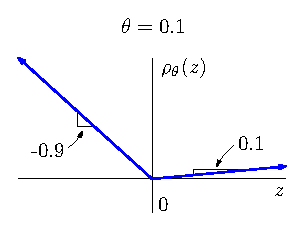
\includegraphics{check-loss-0-1}
  \end{minipage}
  \begin{minipage}[t]{0.33\linewidth}
    \centering
    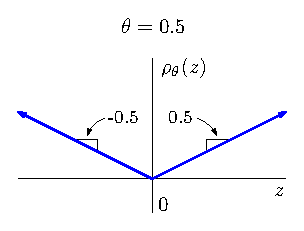
\includegraphics{check-loss-0-5}
  \end{minipage}
  \begin{minipage}[t]{0.33\linewidth}
    \centering
    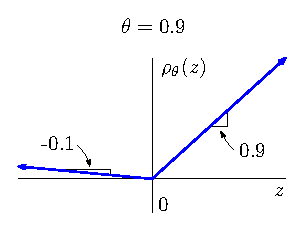
\includegraphics{check-loss-0-9}
  \end{minipage}
  
\end{figure}
Two small examples are provided in Figure \ref{fig:phi-lambda} to further
demonstrate the $\theta$-th quantile classifier and the relationship between the
quantile distances and the difference of the quantile distances.  In these
examples we suppose that $F_0^{-1}(\theta) < F_1^{-1}(\theta)$ at both the 0.25-
and 0.75-th quantile levels, and that $F_1^{-1}(\theta) - F_0^{-1}(\theta)$ is
the same for the two quantile levels.  This is the case for example for
populations that follow $N(0, 1)$ and $N(1, 1)$ distributions.  In the
upper-left plot we show the check loss distance to the populations' 0.25-th
quantiles as a function of input $z$ and denoted as $\Phi_1$ and $\Phi_0$, while
in the bottom-left plot we show the difference of these same check loss
distances, i.e.  $\Lambda = \Phi_1 - \Phi_0$, again as a function of input $z$.
The upper-right and lower right plots also show the check loss distances and
difference between the distances, but instead with respect to the populations'
0.75-th quantiles.  In each of these figures $\tau_{\theta}$ can be seen to
represent the decision rule boundary point, i.e. when $\Lambda = 0$.  We note
that the decision rule boundary is always between $F_{0}^{-1}$ and $F_{1}^{-1}$,
and that when the quantile level is less than 1/2 that $\tau_{\theta}$ is closer
to $F_{1}^{-1}$, and conversely that when the quantile level is greater than 1/2
that $\tau_{\theta}$ is closer to $F_{0}^{-1}$.  Finally, we note that $\Lambda$
is piecewise linear with a slope of $-1$ between $F_{0}^{-1}(\theta)$ and
$F_{1}^{-1}(\theta)$, and is constant otherwise.

Finally, let $Z$ be a random variable with a prior probability $\pi_0$ of being
a member of population $\Pi_0$, and $\pi_1 = 1 - \pi_0$ the prior probability of
being a member of population $\Pi_1$.  Then the probability of correctly
classifying an observed realization of $Z$ by the $\theta$-th quantile
classifier is given by
\begin{equation}
  \label{eq:theoretical-rate}
  \Psi(\theta) =
  \pi_0 \int \ind\Big( \Lambda(z, \theta) > 0 \Big)\, dP_0(z) +
  \pi_1 \int \ind\Big(\Lambda(z, \theta) \leq 0 \Big)\, dP_1(z).
\end{equation}
The expression given in (\ref{eq:theoretical-rate}) has the appealing property
that for the optimal choice of quantile level $\theta$ and under some conditions
that the classification rate is equal to that of the Bayes classifier.  This
result is formally stated in Section \ref{sec:quantile-classifier-optimality} as
Lemma \ref{thm:quantile-classifier-is-bayes}.  We call the quantile classifier
with the optimal quantile level $\theta$ the optimal quantile classifier.  Since
in practice the optimal choice of $\theta$ is unknown, this necessitates the
emprically optimal quantile classifier, which is presented in Section
\ref{sec:empirical-classifier}.


\begin{figure}[ht]
  \caption[cccc]{Example within-class quantile distances and difference in
    quantile distances for two choices of quantiles.
    % In these examples we
    % suppose that $F_0^{-1}(\theta) < F_1^{-1}(\theta)$ for $\theta = 0.25$ and
    % $\theta = 0.75$, and that
    % $F_1^{-1}(0.75) - F_0^{-1}(0.75) = F_1^{-1}(0.25) - F_0^{-1}(0.25)$.  For
    % example, this would be the case when the populations $\Pi_0$ and $\Pi_1$
    % follow $N(0, 1)$ and $N(1, 1)$ distributions, respectively.  In the
    % upper-left plot we show the check loss distance to the populations' 0.25-th
    % quantiles as a function of input $z$ and denoted as $\Phi_1$ and $\Phi_0$,
    % while in the bottom-left plot we show the difference of the check loss
    % distances, $\Lambda = \Phi_1 - \Phi_0$ again as a function of input $z$.
    % The upper-right and lower right plots also show the check loss distances and
    % difference between the distances, but instead with respect to the
    % populations' 0.75-th quantiles.  In each of these figures $\tau_{\theta}$
    % can be seen to represent the decision rule boundary point, which occurs for
    % $\Lambda = 0$.  We note that the decision rule boundary is always between
    % $F_{(0)}^{-1}$ and $F_{(1)}^{-1}$, and that when the quantile level is less
    % than 1/2 that $\tau_{\theta}$ is closer to $F_{(1)}^{-1}$, and conversely
    % that when the quantile level is greater than 1/2 that $\tau_{\theta}$ is
    % closer to $F_{(0)}^{-1}$.  Finally, we note that $\Lambda$ is piecewise
    % linear and that it has a constant value when it is smaller than
    % $F_{(0)}^{-1}$ or larger than $F_{(1)}^{-1}$.
  }

  \label{fig:phi-lambda}
  \vspace{5mm}
  
  \begin{minipage}[t]{0.49\linewidth}
    \centering
    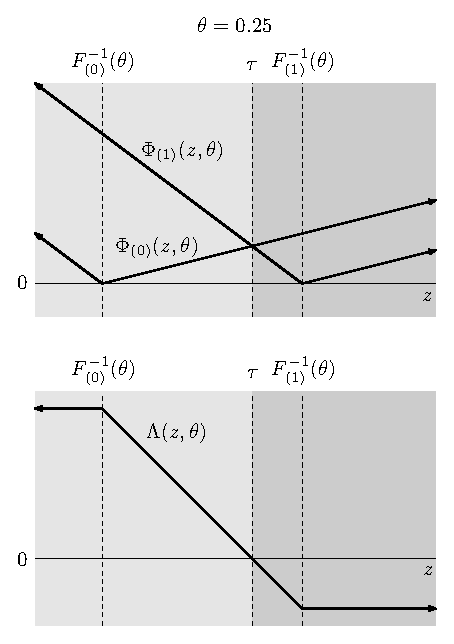
\includegraphics{phi-lambda-0-25}
  \end{minipage}
  \begin{minipage}[t]{0.49\linewidth}
    \centering
    \includegraphics{phi-lambda-0-75}
  \end{minipage}
  
\end{figure}




\subsection{The empirically optimal quantile classifier}
\label{sec:empirical-classifier}

Next we introduce some terminology with which to introduce the sample version of
the optimal quantile classifier.  Let $x_1, \dots, x_m$ be samples from a
population with a probability density on $\mathbb{R}$.  Then we define the
$\theta$-th empirical quantile for the population to be given by any minimizer
of the sample version of equation (\ref{eq:check-loss-min}), defined by
\begin{equation}
  \label{eq:empirical-quantile}
  \hat{F}^{-1} (\theta) = \argmin_q \left\{
    \theta \sum_{ x_{i} > q } |x_{i} - q| ~+~
    (1 - \theta) \sum_{ x_{i} \leq q } |x_{i} - q|
  \right\}.
\end{equation}
It is interesting to note that we can view equation
(\ref{eq:empirical-quantile}) as the solution to a quantile regression problem
introduced in \cite{koenker1978}, where the $x_i$'s correspond to the response
variables, and $q$ is a single regression coefficient corresponding to predictor
data with only an intercept term and no other covariates.  In light of this
fact, we may utilize any of the theory developed in the quantile regression
literature to solve this minimization problem.  However, it turns out that there
is a simple closed-form solution available for this particular special case of
quantile regression, which is presented as Lemma \ref{lem:empirical-quantlev}.

Having defined the $\theta$-th empirical quantile for the population, it follows
that the empirical difference of the quantile distances of a point $z$ to the
population's $\theta$-th quantiles is defined as
\[
  \Lambda_n (z, \theta) = \rho_{\theta}\Big(z - \hat{F}_{1n}^{-1}(\theta)\Big) -
  \rho_{\theta}\Big(z - \hat{F}_{0n}^{-1}(\theta)\Big),
\]
where $\hat{F}_{1n}$ is the estimate of the $\theta$-th quantile level of
population $\Pi_1$ based on the samples in $x_1, \dots, x_n$ that came from
population $\Pi_1$, and similarly for $\hat{F}_{0n}$.  Let $n_0$ and $n_1$
be the number of observations from $\Pi_0$, and $\Pi_1$, respectively.  Then we
further define the observed rate of correct classification for the $\theta$-th
quantile as
\begin{align}
  \begin{split}
    \Psi_n(\theta)
    &= \frac{n_0}{n_0 + n_1} \left[
      \frac{1}{n_0} \sum_{x_i \in \Pi_0}
      \mathbbm{1}\Big( \Lambda_n(x_i, \theta) > 0 \Big)
    \right] +
      \frac{n_1}{n_0 + n_1} \left[
        \frac{1}{n_1} \sum_{x_i \in \Pi_1}
        \mathbbm{1}\Big( \Lambda_n(x_i, \theta) \leq 0 \Big)
      \right] \\[1ex]
    &= \frac{1}{n} \left[
      \sum_{x_i \in \Pi_0} \mathbbm{1}\Big( \Lambda_n(x_i, \theta) > 0 \Big) +
      \sum_{x_i \in \Pi_1} \mathbbm{1}\Big( \Lambda_n(x_i, \theta) \leq 0 \Big)
    \right].
  \end{split}
\end{align}
Finally, define the empirically optimal quantile classifier to be any solution
to the equation
\begin{equation}
  \label{eq:theta-hat}
  \hat{\theta}_n = \argmax_{\theta \in T} \Psi_n(\theta),
\end{equation}
where $T = [\delta, 1 - \delta]$ for some small positive constant $\delta$.  The
restriction of quantile levels to the set $T$ is to guarantee at least one
optimal value of $\theta$ for the theoretical quantile classifier.



% \vspace{10mm} Let $z$ be a univariate observation with a prior
% probability $\pi_0$ of being a member of class 0, and $1 - \pi_0 = \pi_1$ the
% prior probability of being a member of class 1.  Then for quantile level
% $\theta$, define
% \[
%   \rho\,(z, \theta) = \rho_{\theta}\Big(z,\, F_1^{-1}(\theta)\Big) -
%   \rho_{\theta}\Big(z,\, F_0^{-1}(\theta)\Big)
% \]
% Then the probability of a correct classification by the quantile classifier is
% given by
% \begin{equation}
%   \label{eq: theoretical rate}
%   \pi_0 \int \ind\Big( \rho(z, \theta) > 0 \Big)\, dP_0(z) + \pi_1 \int \ind\Big(
%   \rho(z, \theta) \leq 0 \Big) \,dP_1(z)
% \end{equation}
% The expression given in (\ref{eq:theoretical-rate}) has the appealing property
% that for the optimal choice of quantile level $\theta$ the classification rate is
% equal to that of the Bayes classifier.  Thus, to select the quantile level for
% the classification rule given by (\ref{eq:distance-classifier}), one approach
% is to select the empirically optimal choice of $\theta$, as determined by
% leave-one-out cross validation.  To give the definition of this estimator, we
% first describe the setting and introduce some preliminary definitions.

% Consider observations $x_{0, 1}, \dots, x_{0, n_0}$ sampled from population
% $\Pi_0$ and observations $x_{1, 1}, \dots, x_{1, n_1}$ sampled from population $\Pi_1$.
% Then we define
% \[
%   \widehat{\rho}(z, \theta) = \rho_{\theta}\Big(z,\,
%   \widehat{F}_1^{-1}(\theta)\Big) - \rho_{\theta}\Big(z,\,
%   \widehat{F}_0^{-1}(\theta)\Big)
% \]
% where $\widehat{F}_i^{-1}(\theta)$ is estimated from
% $x_{i,1}, x_{i,2}, \dots, x_{i,n_i},~ i = 1, 2$.  Further define
% $\widehat{\rho}_{-x_{i, j}} (z, \theta)$ to be as above, but where
% $\widehat{F}_i^{-1}(\theta)$ is estimated from the data after leaving out the
% $x_{i, j}$ observation (and the estimate of the comparison quantile is
% obtained using the full set of observations from that class).  Then we define
% the empirically optimal quantile level to be given by
% \begin{align}
%   \begin{split}
%     \widehat{\theta^{\text{opt}}}
%     &= \argmax_{\theta \in \{\theta_1, \dots, \theta_K\}} \left\{ \frac{n_0}{n_0 + n_1} \left[ \frac{1}{n_0} \sum_{z \in \Pi_0} \mathbbm{1}\Big( \widehat{\rho}_{-z}(z, \theta) > 0 \Big)  \right] +
%       \frac{n_1}{n_0 + n_1} \left[ \frac{1}{n_1} \sum_{z \in \Pi_1} \mathbbm{1}\Big( \widehat{\rho}_{-z}(z, \theta) \leq 0 \Big)  \right] \right\} \\[1ex]
%     &= \argmax_{\theta \in \{\theta_1, \dots, \theta_K\}} \left\{ \sum_{z \in \Pi_0} \mathbbm{1}\Big( \widehat{\rho}_{-z}(z, \theta) > 0 \Big) +
%       \sum_{z \in \Pi_1} \mathbbm{1}\Big( \widehat{\rho}_{-z}(z, \theta) \leq 0 \Big) \right\}
%   \end{split}
% \end{align}
% for $\theta_1, \dots, \theta_K$ a grid of quantile levels from which to compare.
% Conceptually, $\widehat{\theta^{\text{opt}}}$ is chosen to be the optimizer of
% the sample version of the theoretical optimizer given in equation
% (\ref{eq:theoretical-rate}).

% \begin{editornote}
%   This seems like a reasonable strategy and we have shown empirically that good
%   estimates for the optimal quantile level can be found for a moderate sample
%   size (see project update pdf for 2016-07-01).  However it does have some
%   drawbacks:
  
%   \begin{itemize}
%   \item adds computational burden to the method
%   \item eats up our sample size in that we should set aside training data to
%     train on the quantile estimates
%   \item practical issues with small sample sizes: seems unstable.  Depending on
%     the sample size and the proportion of observations, one class can end up
%     with just a handful or even no observations for a particular class.
%   \end{itemize}
  
% \end{editornote}


% \subsection{Choice of quantile level: distance-based}

% Another approach to selecting the quantile level for the classification rule
% given in expression (\ref{eq: distance classifier}) is based on comparing the
% distances between the quantiles for each class.  Intuitively, the quantiles with
% greater differences between the classes may contain more information in
% discriminating new observations through a comparison of their quantile distances
% to the quantile.  In this section we consider a class of composite
% distance-based quantile levels.

% One major drawback to selecting quantile levels based on a comparison of the
% distances between quantiles is the following.  Consider as an example the case
% where the observations are drawn from populations $\Pi_0$ and $\Pi_1$ such that
% the densities for the populations are $\normal(\mu_0, 1)$ and
% $\normal(\mu_1, 1)$, respectively.  Then
% $\big|F_1^{-1}(\theta) - F_0^{-1}(\theta)\big| = |\mu_1 - \mu_0|$ for all $\theta$. In
% this particular example, the optimal choice of quantile level is 0.5; however,
% when using a distance-based approach to selecting the quantile there is no
% meaningful information from which to make a decision, a clearly undesirable
% property.  However, when extending the classification rule to the multivariate
% setting, there is not a direct connection between the classification problem
% based on one variable and the classification problem drawing information from
% all of the variables, and in practice we may achieve better performance with
% this approach in some settings.

% We propose a class of composite distance-based quantile levels constructed as
% follows.  Consider a grid of quantile levels $\theta_1, \dots, \theta_K$.  Define
% \[
%   d_k = \left| \widehat{F}^{-1}_1 (\theta_k) - \widehat{F}^{-1}_0
%     (\theta_k) \,\right|, \hspace{5mm} k = 1, \dots, K
% \]
% Then a class of component-wise quantile weights is defined as
% \begin{equation}
%   w_k = \frac{ (d_k - \epsilon)_{+}^{\nu} }{ \sum_{\ell = 1}^K (d_{\ell}
%     - \epsilon)_{+}^{\nu} }, \hspace{5mm} k = 1, \dots, K.
% \end{equation}
% where $\nu$ and $\epsilon$ are nonnegative tuning parameters.
% % Various choices
% % of $\nu$ and $\epsilon$ lead to special cases such as
% % \begin{itemize}
% % \item $w_k = 1 / K$
% % \item $\displaystyle w_k = \frac{ (d_k - \epsilon)_+ }
% %   { \sum_{\ell=1}^K (d_{\ell} - \epsilon)_+ }$
% % \item $\displaystyle w_k = \frac{ d_{k}^2 }{ \sum_{\ell=1}^K d_{\ell}^2 }$
% % \end{itemize}
% When using composite quantile levels we write the classifier as follows.  For
% new observation $z$, classify to
% \begin{equation}
%   \label{eq: composite classifier}
%   \left\{ 
%     \begin{array}{lcl}
%       \Pi_0, & & \displaystyle \text{if} \hspace{3mm} \sum_{k=1}^K w_{jk}\,
%                  \bigg\{ \rho_{\theta_k} \left( z - \widehat{F}^{-1}_1 (\theta_k) \right) -
%                  \rho_{\theta_k} \left( z - \widehat{F}^{-1}_0 (\theta_k) \right) \bigg\}
%                  ~>~ 0 \\[2ex]
%       \Pi_1, & & \text{otherwise} \\[1ex]
%     \end{array}
%   \right.
% \end{equation}


% \subsection{Optimal quantile level estimation properties}
% \label{sec: opt quantile est}

% In this section we investigate the finite-sample properties of the leave-one-out
% cross validation approach for estimating the classification rate as a function
% of quantile level.
% \\
% ****  TODO: rework this section if we think it belongs in the paper.  *****
% \\
% \includegraphics[width=1\textwidth]{../../R_Scratch/Plots/Case1.pdf}



\subsection{Optimality and consistency of the quantile classifier}
\label{sec:quantile-classifier-optimality}

With the definitions for the quantile classifier in place, we now provide some
of its properties.  We begin with the fundamental result for the motivation of
the paper, that the quantile classifier achieves the Bayes error rate for the
optimal choice of quantile level.  The following result is due to
\cite{hennig2016}.

\begin{lemma}
  \label{thm:quantile-classifier-is-bayes}
  Consider two populations $\Pi_0$ and $\Pi_1$ with corresponding density
  functions $f_0$ and $f_1$ such that $f_0$ and $f_1$ are nonzero on the same
  domain.  Let $Z$ be a random variable with a prior probability $\pi_0$ of
  being a member of population $\Pi_0$, and $\pi_1 = 1 - \pi_0$ the prior
  probability of being a member of population $\Pi_1$.  Further assume that
  there is a point $z^{*}$ with $\pi_0\, f_0(z^{*}) = \pi_1\, f_1(z^{*})$ so
  that $\pi_0\, f_0(z) < \pi_1\, f_1(z)$ for $z$ on one size of $z^{*}$, and
  $\pi_0\, f_0(z) > \pi_1\, f_1(z)$ on the other side of $z^{*}$.  Then the
  quantile classifier for an observed realization of $Z$ using the optimal
  choice of quantile level achieves the Bayes error rate.
\end{lemma}

Having established the theoretical optimality of the quantile classifier, we now
consider the consistency of the empirical version.  The following result is
essentially a special case of a theorem presented in \cite{hennig2016}.  For
this result, we will need the following assumptions.  Let $\delta$ be a small
positive constant.
\begin{enumerate}[label=\emph{Assumption \arabic*.}, align=left]
\item $F_i^{-1}$ is a continuous function of
  $\theta,~ i=0,1$.
\item $\prob\Big( \Lambda(Z, \theta) = 0 \Big) = 0$ for all
  $\theta \in [\delta, 1 - \delta]$.
\item There is a unique $\tilde{\theta}$ that satisfies $\tilde{\theta} =
  \argmax_{\theta \in T} \Psi(\theta)$.
\end{enumerate}

\begin{lemma}
  \label{lem:univariate-consistency}
  Let $\tilde{\theta}$ be a solution to
  $\tilde{\theta} = \argmax_{\theta \in T} \Psi(\theta)$.  Under Assumptions 1
  and 2, it follows that
  $\Psi(\hat{\theta}_n) \stackrel{p}{\longrightarrow} \Psi(\tilde{\theta})$ with
  $\hat{\theta}_n$ defined in equation (\ref{eq:theta-hat}).  Furthermore, under
  Assumptions 1, 2, and 3, it follows that
  $\hat{\theta}_n \stackrel{p}{\longrightarrow} \tilde{\theta}$.
\end{lemma}

It is worth noting that convergence to the optimal quantile level is based on
the empirically optimal choice for a training data set without the need for
additional training on a validation data set.  Intuitively, this can be
explained by the fact that the model complexity is the same for all of the
possible quantile classifier models, so we do not need to include a model
validation training step to defend against overfitting the model to the data.

% \begin{proof}
%   The fact that
%   $\Psi(\hat{\theta}_n) \stackrel{p}{\longrightarrow} \Psi(\tilde{\theta})$ is a
%   special case of Theorem 1 in \cite{hennig2016} for a feature-space of
%   dimension 1.  Furthermore, during the proof of that theorem it was shown that
%   under Assumptions 1 and 2, $\Psi$ is a continuous function of $\theta$.  To
%   show that $\hat{\theta}_n \stackrel{p}{\longrightarrow} \tilde{\theta}$
%   suppose that the claim doesn't hold.  Then there exists an $\epsilon > 0$ and
%   $\delta > 0$ such that for all $N \in \mathbb{N}$, there exists an $n \geq N$
%   such that
%   \begin{equation*}
%     \prob\Big(
%     \big| \hat{\theta}_n - \tilde{\theta} \big|
%     > \epsilon \Big)
%     \geq \delta.
%   \end{equation*}
%   Now, because $\Psi$ is continuous and $\Psi(\tilde{\theta})$ is a unique
%   maximum, it follows that we can find $\nu > 0$ such that
%   \begin{equation*}
%     \min \left\{
%       \big| \Psi(\Tilde{\theta} - \epsilon) - \Psi(\tilde{\theta}) \big|\,,
%       \hspace{2mm}
%       \big| \Psi(\Tilde{\theta} + \epsilon) - \Psi(\tilde{\theta}) \big|
%     \right\} \geq \nu.
%   \end{equation*}
%   Therefore, for all $N \in \mathbb{N}$, there exists an $n \geq N$ such that
%   \begin{equation*}
%     \prob\Big(
%     \big| \Psi(\hat{\theta}_n) - \Psi(\tilde{\theta}) \big|
%     \geq \nu \Big) \geq
%     \prob\Big(
%     \big| \hat{\theta}_n - \tilde{\theta} \big|
%     \geq \epsilon \Big)
%     \geq \delta.
%   \end{equation*}
%   But this is in contradiction to the fact that
%   $\Psi(\hat{\theta}_n) \stackrel{p}{\longrightarrow} \Psi(\tilde{\theta})$.
% \end{proof}




\subsection{Decision rule calculation}
\label{sec:empirical-quantile-classifier-results}

So far it has been established that the classification rate of the empirically
optimal quantile classifier converges to the classification rate of the true
optimal quantile classifier.  In this section we investigate the practical
considerations of calculating the empirically optimal quantile classifier.  We
begin by providing an expression for the quantile classifier decision rule
boundary in Lemma \ref{lem:decision-boundary}.

\begin{lemma}
  \label{lem:decision-boundary}
  Assume for the moment that $F_{0}^{-1}(\theta) < F_{1}^{-1}(\theta)$.  Then
  the quantile classifier defined in equation (\ref{eq:quantile-classifier}) can
  be equivalently expressed as follows.
  \begin{equation}
    \label{eq:alt-quantile-classifier-less}
    \text{For an observation $z$, classify to:} \hspace{5mm} \left\{ 
      \begin{array}{lcl}
        \Pi_{0}, & & z ~<~ \theta\, F_{0}^{-1}(\theta) +
                       (1 - \theta)\, F_{1}^{-1}(\theta) \\[1ex]
        % \Pi_{1}, & & z ~=~ \theta F_{(0)}^{-1}(\theta) +
        %                (1 - \theta)\, F_{(1)}^{-1}(\theta) \\[1ex]
        \Pi_{1}, & & \textup{otherwise}
      \end{array} .
    \right.
  \end{equation}
  If on the other hand $F_{0}^{-1}(\theta) > F_{1}^{-1}(\theta)$, then the
  direction of the inequality changes so that we instead classify an observation
  to $\Pi_0$ when
  $z ~>~ \theta\, F_{0}^{-1}(\theta) + (1 - \theta)\, F_{1}^{-1}(\theta)$, and
  to $\Pi_1$ otherwise.
  % \begin{equation}
  %   \label{eq:alt-quantile-classifier-greater}
  %   \text{For an observation $z$, classify to:} \hspace{5mm} \left\{ 
  %     \begin{array}{lcl}
  %       \Pi_{0}, & & z ~>~ \theta\, F_{0}^{-1}(\theta) +
  %                    (1 - \theta)\, F_{1}^{-1}(\theta) \\[1ex]
  %                    % \Pi_{1}, & & z ~=~ \theta F_{(0)}^{-1}(\theta) +
  %                    % (1 - \theta)\, F_{(1)}^{-1}(\theta) \\[1ex]
  %       \Pi_{1}, & & \textup{otherwise}
  %     \end{array} .
  %   \right.
  % \end{equation}
\end{lemma}

% \begin{proof}
%   Suppose $F_{(0)}^{-1}(\theta) \ne F_{(1)}^{-1}(\theta)$.  It is clear
%   (e.g. see Figure \ref{fig:phi-lambda}) that $\Phi_{(0)}(z, \theta)$ is
%   equal to $\Phi_{(1)}(z, \theta)$ at exactly one point, say $\tau$, and that
%   the following holds:
%   \begin{equation*}
%     \left\{
%       \begin{array}{lll}
%         \Phi_{(0)}(z, \theta) < \Phi_{(1)}(z, \theta), & & z < \tau \\[1ex]
%         \Phi_{(0)}(z, \theta) = \Phi_{(1)}(z, \theta), & & z = \tau \\[1ex]
%         \Phi_{(0)}(z, \theta) > \Phi_{(1)}(z, \theta), & & z > \tau \\
%       \end{array}
%     \right.
%   \end{equation*}
%   Furthermore, we can infer that
%   $F_{(0)}^{-1}(\theta) < \tau < F_{(1)}^{-1}(\theta)$.  Setting the loss
%   functions equal for $z$ in this interval yields:
%   \begin{align*}
%     & \Phi_{(0)}(z, \theta) \stackrel{\mathit{set}}{=} \Phi_{(1)}(z, \theta) \\
%     & \hspace{5mm} \Longleftrightarrow \hspace{5mm}
%       \ind\!\! \left(z > F_{(0)}^{-1}(\theta)\right) \theta
%       \left(z - F_{(0)}^{-1}(\theta)\right) +
%       \ind\!\! \left(z \leq F_{(0)}^{-1}(\theta)\right) (1 - \theta)
%       \left(F_{(0)}^{-1}(\theta) - z\right) \\
%     & \hspace{25mm} =
%       \ind\!\! \left(z > F_{(1)}^{-1}(\theta)\right) \theta
%       \left(z - F_{(1)}^{-1}(\theta)\right) +
%       \ind\!\! \left(z \leq F_{(1)}^{-1}(\theta)\right) (1 - \theta)
%       \left(F_{(1)}^{-1}(\theta) - z\right) \\
%     & \hspace{5mm} \Longleftrightarrow \hspace{5mm}
%       \theta \left(z - F_{(0)}^{-1}(\theta)\right) =
%       (1 - \theta) \left(F_{(1)}^{-1}(\theta) - z\right) \\
%     & \hspace{5mm} \Longleftrightarrow \hspace{5mm}
%       z = \theta\, F_{(0)}^{-1}(\theta) + (1 - \theta)\, F_{(1)}^{-1}(\theta).
%   \end{align*}
%   It can then be verified that $\Phi_{(0)}(z, \theta) < \Phi_{(1)}(z, \theta)$
%   corresponds to classifying $z$ to $\Pi_{(0)}$ and that
%   $\Phi_{(0)}(z, \theta) > \Phi_{(1)}(z, \theta)$ corresponds to classifying $z$
%   to $\Pi_{(1)}$.  Combining these facts yields the desired result.
% \end{proof}
It is interesting to note that the decision rule boundary lies on the line
segment between $F_0^{-1}(\theta)$ and $F_1^{-1}(\theta)$, with the location of
the point on the line segment determined by the quantile level.  We saw an
example of this in Figure \ref{fig:phi-lambda} in that for the 0.25-th quantile
level the decision rule boundary was closer to the larger quantile, and for the
0.75-th quantile level the decision rule boundary was closer to the smaller
quantile.

Next, the result given in Lemma \ref{lem:empirical-quantlev} provides an
expression with which to obtain an optimal solution for the empirical quantile
estimator.  

\begin{lemma}
  \label{lem:empirical-quantlev}
  Let $x_1, \dots, x_m$ be points on $\mathbb{R}$.  Then a solution to equation
  (\ref{eq:empirical-quantile}) providing the $\theta$-th empirical quantile for
  $x_1, \dots, x_m$ is given by $\lceil m \theta \rceil$-th largest value of the
  $x_i$.
\end{lemma}

% \begin{proof}
%   % 
We can write the minimization problem
\begin{equation*}
  \min_q \left\{
    \theta \sum_{ x_{i} > q } |x_{i} - q| ~+~
    (1 - \theta) \sum_{ x_{i} \leq q } |x_{i} - q|
  \right\}
\end{equation*}
equivalently as
% \begin{align*}
%   &\min_{q^{+}, q^{-}, \vec{u}, \vec{v}} \left\{
%     \theta \sum_{i=1}^m u_i ~+~
%     (1 - \theta) \sum_{i=1}^m v_i
%   \right\} \\[2ex]
%   & \text{subject to} \hspace{3mm}
%   x_i - (q^{+} - q^{-}) = u_i - v_i, \hspace{5mm} i = 1, \dots, m \\[2ex]
%   & q^{+} \geq 0,~ q^{-} \geq 0,~ \vec{u} \geq \vec{0},~ \vec{v} \geq 0
% \end{align*}
\begin{equation*}
  \arraycolsep=5mm
  \begin{array}{ll}
    \displaystyle
    \minimize_{q^{+}, q^{-}, \vec{u}, \vec{v}}
    & \theta \sum_{i=1}^m u_i ~+~
      (1 - \theta) \sum_{i=1}^m v_i \\[2ex]
    \text{subject to}
    & x_i - (q^{+} - q^{-}) = u_i - v_i, \hspace{5mm} i = 1, \dots, m \\[2ex]
    & q^{+} \geq 0,~ q^{-} \geq 0,~ \vec{u} \geq \vec{0},~ \vec{v} \geq \vec{0} \\
  \end{array}
\end{equation*}
which is seen to be a linear programming problem in standard form.  By rewriting
the equality condition as $q^{+} - q^{-} + u_i - v_i = x_i$ for $i=1, \dots, m$,
we can express the equality condition in matrix form as
\begin{equation*}
  \begin{bmatrix}
    1      & -1     & 1 &        &   & -1 &        &    \\
    \vdots & \vdots &   & \ddots &   &    & \ddots &    \\
    1      & -1     &   &        & 1 &    &        & -1 \\
  \end{bmatrix}
  % \begin{bmatrix}
  %   q^{+} \\ q^{-} \\ u_{1} \\ \vdots \\ u_m \\ v_1 \\ \vdots \\ v_m \\
  % \end{bmatrix}
  \begin{bmatrix}
    q^{+} \\ q^{-} \\ \vec{u} \\ \vec{v} \\
  \end{bmatrix}
  =
  \begin{bmatrix}
    x_1 \\ \vdots \\ x_m \\
  \end{bmatrix}.
\end{equation*}
% \begin{equation*}
%   \begin{bmatrix}
%     1      & -1     & 1         &        &  \bigDown{0} & -1        &        & \bigDown{0} \\
%     \vdots & \vdots &           & \ddots &              &           & \ddots &             \\
%     1      & -1     & \bigUp{0} &        & 1            & \bigUp{0} &        & -1          \\
%   \end{bmatrix}
% \end{equation*}
% \begin{equation*}
%   \begin{bmatrix}
%     1      & -1     & &         &  & &          & \\
%     \vdots & \vdots & & \vec{I} &  & & -\vec{I} & \\
%     1      & -1     & &         &  & &          & \\
%   \end{bmatrix}
% \end{equation*}
% \begin{equation*}
%   \begin{bmatrix}
%     1      & -1     & 1      & 0      & \dots  & 0       & -1     &        &    \\
%     \vdots & \vdots & 0      & \ddots & \ddots & \vdots  &  0     & \ddots & \\
%     \vdots & \vdots & \vdots & \ddots & \ddots & 0       & \vdots & \ddots & \ddots &    \\
%     1      & -1     & 0      & \dots  & 0      & 1       &  0     & \dots  &  0     & -1 \\
%   \end{bmatrix}
% \end{equation*}
Recall that a solution for $(q^{+}, q^{-}, \vec{u}, \vec{v})$ is a basic
solution if and only if there exist indices $B(1), \dots, B(m)$ such that both
(i) the columns of the coefficient matrix with column indices subset by
$B(1), \dots, B(m)$ are linearly independent, and (ii) if an element of
$(q^{+}, q^{-}, \vec{u}, \vec{v})$ does not correspond to one of
$B(1), \dots, B(m)$ then the element must have a value of 0.

We can see that in order to have independent columns from the coefficient
matrix, then for each $i$, no more than one of the columns corresponding to
either $u_i$ or $v_i$ can have an index in $B(1), \dots, B(m)$, and additionally
no more than one of the columns corresponding to either $q^{+}$ or $q^{-}$ can
have an index in $B(1), \dots, B(m)$.  Furthermore, we note that if we have one
column corresponding to $q^{+}$ or $q^{-}$, and one column corresponding to
either $u_i$ or $v_i$ for each $i$, then we have $m + 1$ columns, which is still
one column too many.  Thus we see that there must be either (i) exactly one
column corresponding to either $u_i$ or $v_i$ for each $i$ and no columns
corresponding to either $q^{+}$ or $q^{-}$, or (ii) exactly one column
corresponding to either $u_i$ or $v_i$ for each $i$ less one and exactly one
column corresponding to either $q^{+}$ or $q^{-}$.

% Next we notice that if we include a column corresponding to $q^{+}$ or $q^{-}$,
% then the solution for the corresponding coefficient is either the value of $x_i$
% or $-x_i$, and where the index $i$ corresponds to the only $i$ without a column
% corresponding to either $u_i$ or $v_i$.  Then each

Furthermore, we can infer that if a column corresponding to $q^{+}$ or $q^{-}$
has an index in $B(1), \dots, B(m)$ and the solution is feasible (i.e. $q^{+}$
and $q^{-}$ are both nonnegative), then $q^{+} = (x_i)_{+}$ and
$q^{-} = (-x_i)_{+}$, where the index $i$ corresponds to the only $i$ without a
column corresponding to either $u_i$ or $v_i$, and $(z)_{+} = \max(0, z)$.  Let
$q = q^{+} - q^{-}$, then it follows that a feasible solution for any $j \ne i$
has $u_i = (x_i - q)_{+}$ and $v_i = (q - x_i)_{+}$.  This leads to a set of
basic feasible solutions given by $q \in \{x_1, \dots, x_m\}$.  One last basic
feasible solution is given for $q = 0$ with $u_i = (x_i)_{+}$ and
$v_i = (-x_i)_{+}$ for all $i$.

Next we aim to find the minimizing basic feasible solution.  Suppose that
$\lceil \theta m \rceil = k$ and that $\ell < k$, and let $q = x_k$ and
$q^{\prime} = x_{\ell}$.  Then comparing the objective function evaluated at $q$
and $q^{\prime}$, we have
\begin{align*} 
  \left\{ \theta \sum_{i=\ell+1}^m \right.
  & (x_i - q^{\prime}) +
    \left. (1 - \theta) \sum_{i=1}^{\ell} (q^{\prime} - x_i) \right\} -
    \left\{ \theta \sum_{i=k+1}^m (x_i - q) +
    (1 - \theta) \sum_{i=1}^k (q - x_i) \right\} \\[1ex]
  &= (1 - \theta) \sum_{i=1}^{\ell} \Big\{ (q^{\prime} - x_i) - (q - x_i) \Big\} \\
  &\hspace{8mm}
    + \theta \sum_{i=\ell+1}^k (x_i - q^{\prime})
    - (1 - \theta) \sum_{i=\ell+1}^k (q - x_i) \\
  &\hspace{8mm}
    + \theta \sum_{i=k+1}^m \Big\{ (x_i - q^{\prime})
    - (x_i - q) \Big\} \\[1ex]
  % &= (1 - \theta) \sum_{i=1}^{\ell} \Big\{ (q^{\prime} - x_i) - (q - x_i) \Big\} \\
  % &\hspace{8mm}
  %   + \theta \sum_{i=\ell+1}^k (x_i - q^{\prime})
  %   - (1 - \theta) \sum_{i=\ell+1}^k (q - x_i) \\
  % &\hspace{8mm}
  %   + (1 - \theta) \sum_{i=\ell+1}^k (q^{\prime} - x_i)
  %   - (1 - \theta) \sum_{i=\ell+1}^k (q^{\prime} - x_i) \\
  % &\hspace{8mm}
  %   + \theta \sum_{i=k+1}^m \Big\{ (x_i - q^{\prime})
  %   - (x_i - q) \Big\} \\[1ex]
  &= (1 - \theta) \sum_{i=1}^{\ell} \Big\{ (q^{\prime} - x_i) - (q - x_i) \Big\} \\
  &\hspace{8mm}
    + \theta \sum_{i=\ell+1}^k (x_i - q^{\prime})
    - (1 - \theta) \sum_{i=\ell+1}^k (q - x_i)
    \pm (1 - \theta) \sum_{i=\ell+1}^k (q^{\prime} - x_i) \\
  &\hspace{8mm}
    + \theta \sum_{i=k+1}^m \Big\{ (x_i - q^{\prime})
    - (x_i - q) \Big\} \\[1ex]
  &= -(1 - \theta) \sum_{i=1}^{\ell}\, (q - q^{\prime}) \\
  &\hspace{8mm}
    + \theta \sum_{i=\ell+1}^k (x_i - q^{\prime})
    - (1 - \theta) \sum_{i=\ell+1}^k (q - q^{\prime})
    - (1 - \theta) \sum_{i=\ell+1}^k (q^{\prime} - x_i) \\
  &\hspace{8mm}
    + \theta \sum_{i=k+1}^m (q - q^{\prime}) \\[1ex]
  &= -(1 - \theta) \sum_{i=1}^k\, (q - q^{\prime}) \\
  &\hspace{8mm}
    + \theta \sum_{i=\ell+1}^k (x_i - q^{\prime})
    - (1 - \theta) \sum_{i=\ell+1}^k (q^{\prime} - x_i) \\
  &\hspace{8mm}
    + \theta \sum_{i=k+1}^m (q - q^{\prime}) \\[1ex]
  &= -(1 - \theta) \sum_{i=1}^k\, (q - q^{\prime}) \\
  &\hspace{8mm}
    + \sum_{i=\ell+1}^k (x_i - q^{\prime}) \\
  &\hspace{8mm}
    + \theta \sum_{i=k+1}^m (q - q^{\prime}) \\[1ex]
  & = - (1 - \theta)\, k\, (q - q^{\prime})
    + \sum_{i=\ell+1}^k (x_i - q^{\prime})
    + \theta (m - k) (q - q^{\prime}) \\
  &= \sum_{i=\ell+1}^k (x_i - q^{\prime}) - (k - \theta m) (q - q^{\prime}) \\
  &\geq (x_k - q^{\prime}) - (q - q^{\prime}) \\
  &= x_k - q \\
  &= 0
\end{align*}
The inequality is due to the fact that $x_i \geq q^{\prime}$ for
$i \geq \ell + 1$, and also the fact that $k - \theta m < 1$.  Suppose now that
$\lceil \theta m \rceil = k$ and that $\ell > k$, and let $q = x_k$ and
$q^{\prime} = x_{\ell}$.  Then comparing the objective function evaluated at $q$
and $q^{\prime}$, we have
\begin{align*} 
  \left\{ \theta \sum_{i=\ell+1}^m \right.
  & (x_i - q^{\prime}) +
    \left. (1 - \theta) \sum_{i=1}^{\ell} (q^{\prime} - x_i) \right\} -
    \left\{ \theta \sum_{i=k+1}^m (x_i - q) +
    (1 - \theta) \sum_{i=1}^k (q - x_i) \right\} \\[1ex]
  &= (1 - \theta) \sum_{i=1}^k \Big\{ (q^{\prime} - x_i) - (q - x_i) \Big\} \\
  &\hspace{8mm}
    + \theta \sum_{i=k+1}^{\ell} (x_i - q^{\prime})
    - (1 - \theta) \sum_{i=k+1}^{\ell} (q - x_i) \\
  &\hspace{8mm}
    + \theta \sum_{i=\ell+1}^m \Big\{ (x_i - q^{\prime})
    - (x_i - q) \Big\} \\[1ex]
  &= (1 - \theta) \sum_{i=1}^k\, (q^{\prime} - q) \\
  &\hspace{8mm}
    - \theta \sum_{i=k+1}^{\ell} (q^{\prime} - q)
    + \sum_{i=k+1}^{\ell} (x_i - q) \\
  &\hspace{8mm}
    - \theta \sum_{i=l+1}^m (q^{\prime} - q) \\[1ex]
  % &= (1 - \theta) \sum_{i=1}^k\, (q^{\prime} - q) \\
  % &\hspace{8mm}
  %   + \sum_{i=k+1}^{\ell} (x_i - q) \\
  % &\hspace{8mm}
  %   - \theta \sum_{i=k+1}^m (q^{\prime} - q) \\[1ex]
  &= (1 - \theta) \sum_{i=1}^k\, (q^{\prime} - q)
    + \sum_{i=k+1}^{\ell} (x_i - q)
    - \theta \sum_{i=k+1}^m (q^{\prime} - q) \\
  &= (1 - \theta)\, k\, (q^{\prime} - q)
    + \sum_{i=k+1}^{\ell} (x_i - q)
    - \theta\, (m - k) (q^{\prime} - q) \\
  &= (k - \theta m) (q^{\prime} - q) + \sum_{i=k+1}^{\ell} (x_i - q) \\
  &\geq 0
\end{align*}
There is one basic feasible solution remaining to check, that where $q = 0$.  To
show that this is not the optimal solution except in the case that
$x_{\lceil \theta m \rceil} = 0$, we make the following argument.  Note that if
we add some nonzero value $\tau$ to each $x_i$ and if $q^{*}$ is an optimal
choice for the original problem, then $q^{*} + \tau$ is an optimal choice for
the new problem.  Choose $-\tau$ to be one of the $x_i$ for some $i$: then 0 is
one of the values in the transformed data, which was shown in the previous
results to be no better than the $\lceil \theta m \rceil$-th largest value of
the transformed data, so it follows that the $\lceil \theta m \rceil$-th largest
value is optimal.  Since $\tau$ cannot be better than optimal for the transormed
data, then by the law of the contrapositive 0 cannot be better than optimal for
the original data.




%%% Local Variables:
%%% mode: latex
%%% TeX-master: "cqc_paper"
%%% End:

%   The proof is relegated to the supplementary materials.  The result is
%   essentially a consequence of the fact that the problem can be cast as a linear
%   programming problem where the extreme points of the feasible set are the
%   values of the $x_i$.
% \end{proof}

Futhermore, as a consequence of the results of Lemmas
\ref{lem:decision-boundary} and \ref{lem:empirical-quantlev}, the result in
Lemma \ref{lem:decision-rule-time} characterizes the complexity of obtaining the
empirical decision rule boundary for a given dataset.

\begin{lemma}
  \label{lem:decision-rule-time}
  Obtaining the quantile classifier decision rule boundary for a fixed choice of
  quantile level is an $\bigO(n)$ operation.
\end{lemma}

% \begin{proof}
%   Constructing the $\theta$-th quantile classifier requires merely finding the
%   $\lceil \theta n_0 \rceil$-th largest value from the observations that were
%   drawn from population $\Pi_0$, and the $\lceil \theta n_1 \rceil$-th largest
%   value from the observations that were drawn from population $\Pi_1$, and then
%   calculating the decision boundary based on Lemma \ref{lem:decision-boundary}.
%   Finding the $k$-th largest value of a set is an $\bigO(n)$ operation, and the
%   calculation to obtain the decision boundary using Lemma
%   \ref{lem:decision-boundary} is an $\bigO(1)$ operation.
% \end{proof}




\subsection{Calculating the empirically optimal quantile classifier}
\label{sec:empirically-optimal-algo}

Given the availability of a closed-form expression for the decision rule
boundary at a fixed quantile level, an immediately apparent question is whether
an empirically optimal quantile classifier can be efficiently obtained.
Intuitively, we can sort the data and simply ``slide'' the decision rule
boundary across the range of the data, counting the number of data points for
either class on the correct side of the boundary to find an optimal choice.
Furthermore, since the classification rate doesn't change as we slide the
decision boundary in-between observations, we need only calculate the
classification rate for some countable number of decision boundary choices.

A sketch of the procedure to calculate the empirical classification rate over
the entire space of quantile levels is presented below, and a more detailed
description is provided in the supplementary materials.  The basic idea is that
the quantile estimates $\hat{F}_0^{-1}$ and $\hat{F}_1^{-1}$ are step functions
with respect to the quantile level and with change points occuring on the sets
$\left\{\frac{1}{n_0}, \dots, \frac{n_o - 1}{n_0}\right\}$ and
$\left\{\frac{1}{n_1}, \dots, \frac{n_1 - 1}{n_1}\right\}$, respectively.  Thus
for intervals not containing any of these points except as endpoints, the
quantile estimates are fixed and the interval can be mapped to a contiguous
interval of decision rule boundaries.  Within these decision rule boundary
intervals we can further partition a given interval into sub-intervals that each
has a constant empirical classification rate by letting the partition boundaries
be defined by any data points contained in the interval.  Thus by counting the
number of data points from each class on either side of the decision boundary
for every sub-interval we obtain the empirical classification rate over the
entire quantile level space.  A high-level version of the algorithm is presented
as Algorithm \ref{alg:empirically-optimal-classifier}, and a result for the
algorithm complexity is presented as Proposition
\ref{lem:optimal-quantile-time}.

An illustrative example for a small data set is presented as Figure
\ref{fig:empirical-classification-rate} showing the decision rule boundary and
corresponding classification rate as a function of the quantile level.  A data
set for class 0 with 7 observations was sampled from independent $N(0, 1)$
distributions yielding the values
$-0.96,\allowbreak -0.78,\allowbreak -0.46,\allowbreak -0.10,\allowbreak
0.24,\allowbreak 0.98,\allowbreak 1.61$, and a data set for class 1 with 5
observations was sampled from independent $N(1, 1)$ distributions yielding the
values
$-0.60,\allowbreak 0.37,\allowbreak 0.64,\allowbreak 1.37,\allowbreak 1.78$.
These values are shown as the horizontal lines in the top panel, along with the
decision rule boundaries corresponding to this data which are displayed as the
diagonal blue lines.  The dashed vertical lines represent the quantile levels at
which the quantile estimates change for at least one of the classes.  In the
bottom panel the number of correctly classified observations out of a possible
12 observations is plotted as a function of the quantile level.  From this
figure we see that the classification rate of the quantile classifier is
constant for the intervals between the quantile estimate change points except
when the set of corresponding decision rule boundary values includes values in
the data.  When this is the case the intervals can be further divided into
sub-intervals with a constant classification rate.  For this particular example
the theoretically optimal quantile level is 0.5, which is indeed one of the
empirically optimal quantile levels.

One issue that has yet to be addressed that is evident in this example is how to
choose a quantile level based on a training data set when there is more than one
empirically optimal value.  When this is the case, as it typically is, we find
that selecting the value closest to the median works well in many settings.  One
argument for this choice is that the median is the optimal choice of quantile
level for two classes with symmetric distributions that differ only by a
location shift.  While this scenario may not hold in many settings, it still
offers in some sense a conservative rule for what is hopefully a small set of
empirically quantile levels from which to choose.

\begin{figure}[p]
  \caption[Example empirical classification rate]{Illustrative plot of the
    empirical classification rate for a toy example.  An example data set is
    shown with 7 values from class $\Pi_0$ and 5 values from class $\Pi_1$. }
  \label{fig:empirical-classification-rate}
  \centering
  \vspace{5mm}

  \includegraphics[width=1\textwidth]{emp_quant_example}
\end{figure}


% \begin{algorithm}[p]
%   \label{alg:empirically-optimal-classifier}
%   \DontPrintSemicolon
%   \BlankLine
%   % \KwResult{Write here the result}
%   \SetKwInOut{Input}{Data}
%   % \SetKwInOut{Output}{Output}
%   \Input{$v_1, \dots, v_{n_0}$ from $\Pi_0$ and $w_1, \dots, w_{n_1}$ in
%     $\Pi_W$}
%   % \Output{Write here the output}
%   % \BlankLine
  
%   sort observations $v_1, \dots, v_{n_0}$ and $w_1, \dots, w_{n_1}$.  Assume
%   that in the case of ties, we classify to $\Pi_W$. \;
  
%   sort $x_1, \dots, x_r$ a collection of the unique values from among the $v_i$
%   and $w_i$, and track how many $v_i$ and how many $w_i$ are less than each
%   $x_j$ \;
  
%   calculate in such a way so as to produce a sorted set of quantile levels given by
%   \begin{equation*}
%     \Theta = \Big\{ 0 \Big\} \bigcup
%     \left\{ \frac{k}{n_0}: 1 \leq k \leq n_0 \right\} \bigcup
%     \left\{ \frac{k}{n_1}: 1 \leq k \leq n_1 \right\}
%   \end{equation*}

%   \For{$i$ in 2 to $|\Theta|$}{
    
%     \BlankLine
    
%     calculate $\hat{F}_V^{-1}(\theta_i)$ and $\hat{F}_W^{-1}(\theta_i)$, and
%     find
%     \begin{equation*}
%       a = \min \Big\{ \hat{F}_0^{-1}(\theta_i),~ \hat{F}_1^{-1}(\theta_i) \Big\}
%       \hspace{5mm} \text{and} \hspace{5mm}
%       b = \max \Big\{ \hat{F}_0^{-1}(\theta_i),~ \hat{F}_1^{-1}(\theta_i) \Big\}
%     \end{equation*}

%     calculate the interval
%     \[
%       G_i = \Big[
%       \theta_i\, a + (1 - \theta_i)\, b,
%       \hspace{3mm}
%       \theta_{i-1}\, a + (1 - \theta_{i-1})\, b\,
%       \Big) = \big[x_{\scriptscriptstyle\text{low}},\,
%       x_{\scriptscriptstyle\text{high}}\big)
%     \]
%     % Let $x_{\scriptscriptstyle\text{low}}$ and
%     % $x_{\scriptscriptstyle\text{high}}$ denote the lower and upper bounds of $G_i$,
%     % respectively.  \;

%     find the smallest $x_i \in [x_{\scriptscriptstyle\text{low}}, \infty)$.  If
%     $x_i \geq x_{\scriptscriptstyle\text{high}}$ then calculate the
%     classification rate for $G_i$.

%     \BlankLine

%     \While{$x_i \in G_i$}{

%       calculate the classification rate for the interval with upper and lower
%       bounds determined by $x_i$ and
%       $\min\{x_{i+1}, x_{\scriptscriptstyle\text{high}}\}$, respectively (for
%       whether bounds in interval are open or closed see below)

%       \BlankLine

%       \uIf{$\hat{F}_V^{-1}(\theta_i) < \hat{F}_W^{-1}(\theta_i)$}{
%         % partition $G_i$ into the following intervals each with a constant
%         % classification rate \vspace{-2mm}
%         calculate classification rate for the interval with bounds $x_i$ and
%         $x_{i+1}$ among the following:
%         \begin{equation*}
%           [x_{\scriptscriptstyle\text{low}}, x_k],\, (x_k, x_{k+1}],\, \dots,\,
%           (x_{k+s-1}, x_{k+s}],\, (x_{k+s},\, x_{\scriptscriptstyle\text{high}})
%         \end{equation*}
%       }
%       \Else{
%         % partition $G_i$ into the following intervals each with a constant
%         % classification rate \vspace{-2mm}
%         calculate classification rate for the interval with bounds $x_i$ and
%         $x_{i+1}$ among the following:
%         \begin{equation*}
%           [x_{\scriptscriptstyle\text{low}}, x_k),\, [x_k, x_{k+1}),\, \dots,\,
%           [x_{k+s-1}, x_{k+s}),\, [x_{k+s},\, x_{\scriptscriptstyle\text{high}})
%         \end{equation*}
%       }

%       map interval back to corresponding interval in the quantile levels space \;
      
%       $x_i \leftarrow x_{i+1}$
            
%     }
    
%   }
%   \caption{calculate the empirically optimal quantile classifer}
% \end{algorithm}


\begin{algorithm}[ht]
  \caption{Calculating the empirically optimal quantile classifer}
  \label{alg:empirically-optimal-classifier}
  \DontPrintSemicolon
  \BlankLine
  \SetKwInOut{Input}{Data}
  \Input{$v_1, \dots, v_{n_0}$ from $\Pi_0$ and $w_1, \dots, w_{n_1}$ in
    $\Pi_1$}
  
  % sort observations $v_1, \dots, v_{n_0}$ and $w_1, \dots, w_{n_1}$ \;
  
  % Sort $x_1, \dots, x_r$ a collection of the unique values from among the $v_i$
  % and $w_i$ \;

  Sort $v_1, \dots, v_{n_0}, w_1, \dots, w_{n_1}$ and denote the unique values
  as $x_1, \dots, x_r$
  
  Produce a sorted set of quantile levels given by
  $ \Theta = \Big\{ 0 \Big\} \bigcup \left\{ \frac{k}{n_0}: 1 \leq k \leq n_0
  \right\} \bigcup \left\{ \frac{k}{n_1}: 1 \leq k \leq n_1 \right\} $

  \BlankLine

  \For{$i$ in 2 to $|\Theta|$}{
    
    \BlankLine
    
    calculate $\hat{F}_V^{-1}(\theta_i)$ and $\hat{F}_W^{-1}(\theta_i)$, and
    find \vspace{-0mm}
    \begin{equation*}
      a = \min \Big\{ \hat{F}_0^{-1}(\theta_i),~ \hat{F}_1^{-1}(\theta_i) \Big\}
      \hspace{5mm} \text{and} \hspace{5mm}
      b = \max \Big\{ \hat{F}_0^{-1}(\theta_i),~ \hat{F}_1^{-1}(\theta_i) \Big\}
    \end{equation*}
    \vspace{-5mm}
    
    calculate the interval
    \vspace{-0mm}
    \[
      G_i = \Big[
      \theta_i\, a + (1 - \theta_i)\, b,
      \hspace{3mm}
      \theta_{i-1}\, a + (1 - \theta_{i-1})\, b\,
      \Big) = \big[x_{\scriptscriptstyle\text{low}},\,
      x_{\scriptscriptstyle\text{high}}\big)
    \]
    % Let $x_{\scriptscriptstyle\text{low}}$ and
    % $x_{\scriptscriptstyle\text{high}}$ denote the lower and upper bounds of $G_i$,
    % respectively.  \;

    partition
    $\big[x_{\scriptscriptstyle\text{low}},\,
    x_{\scriptscriptstyle\text{high}}\big)$ where the partition boundaries are
    given by any $x_i$ in the interval, and calculate the classification rate
    for each sub-interval
    
  }
\end{algorithm}


\begin{proposition}
  \label{lem:optimal-quantile-time}
  The decision rule for the empirically optimal quantile classifier can be
  obtained in $\mathcal{O}(n^2)$ time.
\end{proposition}

% \begin{proof}
%   Sorting the data is an $\mathcal{O}(n \log n)$ operation.  The operations
%   performed in line 2 of Algorithm \ref{alg:empirically-optimal-classifier}
%   takes $\mathcal{O}(n)$ time.

%   The outer loop beginning on line 3 of Algorithm
%   \ref{alg:empirically-optimal-classifier} requires some number of iterations
%   that is bounded from above by $n - 1$.  Within each iteration, calculating
%   $F_V^{-1}$ and $F_W^{-1}$ and the interval $G_i$ are each constant time
%   operations.

%   The step in line 6 of Algorithm \ref{alg:empirically-optimal-classifier} is
%   really a high-level view of a second loop.  This inner loop requires first
%   finding the set of $x_i$'s with values in
%   $\big[x_{\scriptscriptstyle\text{low}},\,
%   x_{\scriptscriptstyle\text{high}}\big)$ which is an $\mathcal{O}(\log n)$
%   operation.  The number of times that the inner loop is performed is determined
%   by the number of points with values in the interval and is bounded from above
%   by $n - 1$.  Calculating the classification rate the sub-interval in each step
%   of the inner loop is a constant time operation, as is mapping the sub-interval
%   back to the quantile levels space.

%   So combining the worst-case bound for the outer and inner loops, we find that
%   the total number of intervals for which we calculate the classification rate
%   for has a worst-case bound on the order of $n^2$ intervals, and that each
%   calculation is a constant time operation for a total cost of
%   $\mathcal{O}(n^2)$ time.  The initial operations performed in lines 1-2 of
%   Algorithm \ref{alg:empirically-optimal-classifier} have an aggregate cost with
%   $\mathcal{O}(n \log n)$ time, so in total the algorithm runs in
%   $\mathcal{O}(n^2)$ time.
% \end{proof}

It remains an open question as to whether the bound obtained in Proposition
\ref{lem:optimal-quantile-time} is actually achievable.  In practice, for both
simulated and real data we typically see less than $n$ total intervals that need
to be considered in the outer and inner loops, so when this is the case the
algorithm runs in $\mathcal{O}(n \log n)$ time.  As an alternative, we can
approximate the empirically optimal quantile classifier by simply calculating
the empirical classification rate over a fine grid of quantile levels, which
reduces the complexity to an $\mathcal{O}(Kn)$ operation where $K$ is the number
of points in the grid.  This complexity is the case because each choice of
quantile level requires calculating the decision rule boundary by finding the
$k_0$-th and $k_1$-th largest value of each class for the appropriate values of
$k_0$ and $k_1$, and then counting the number of observations on the correct
side of the boundary, each of which is an $\mathcal{O}(n)$ operation.




%%% Local Variables:
%%% mode: latex
%%% TeX-master: "cqc_paper"
%%% End:



\section{Quantile-based classifiers for multivariate data}
\label{sec:multivariate-classifier}

Having characterized the inherently univariate quantile classifier, our goal
then is to construct a classification method for data with multivariate features
based upon the quantile classifier.  We begin by extending some of the notation
from the previous section to the multivariate setting.

First, consider two populations $\Pi_0$ and $\Pi_1$ with corresponding
distribution functions $F_0$ and $F_1$ each on $\mathbb{R}^{p}$, and further let
$F_{0j}$ and $F_{1j}$ denote the marginal distribution functions for the $j$-th
variable with respect to $F_0$ and $F_1$, $j = 1, \dots, p$.  Then we denote the
quantile distance of a point $z \in \mathbb{R}$ to the $\theta$-th quantile of a
population's $j$-th component as
\begin{equation}
  \label{eq:multivariate-phi}
  \Phi_{ij}(z, \theta) =
  \rho_{\theta}\Big(z - F_{ij}^{-1}(\theta) \Big),
  \hspace{5mm} i = 0, 1, \hspace{3mm} j = 1, \dots, p.
\end{equation}
Then the difference of the quantile distances of a point $z$ to the populations'
$\theta$-th quantile of the $j$-th component is defined as
\begin{equation}
  \Lambda_j (z, \theta) = \Phi_{1j}(z, \theta) - \Phi_{0j}(z, \theta),
  \hspace{5mm} j = 1, \dots, p.
\end{equation}
The main idea then of the composite quantile-based classifiers proposed in the
next section is to aggregate the discriminatory information contained in each of
the $\Lambda_j$'s so as to construct a classification method for data with
multivariate features.


\subsection{Composite quantile-based classifiers}
\label{sec:varying-coefficient}

In this section we propose the composite quantile-based classifiers
family; we start by motivating the the form of the classifiers.  Consider a
point $\vec{z} = (z_1, \dots, z_p) \in \mathbb{R}^p$ and quantile levels
$\vec{\theta} = (\theta_1, \dots, \theta_p) \in (0, 1)^p$.  Then the difference
of the quantile distances of the $j$-th component of $\vec{z}$ to the
populations' $\theta_j$-th quantile of the $j$-th component
$\Lambda_j(z_j, \theta_j)$ provides some discriminatory information for the
classification of $\vec{z}$.  In more detail, if $\Lambda_j(z_j, \theta_j)$ is a
large positive value (large relative to the magnitude of the $j$-th component),
then this indicates that $z_j$ is much closer to the $\theta_j$-th quantile of
the $j$-th component of population $\Pi_0$ than it is to the $\theta_j$-th
quantile of the $j$-th component of population $\Pi_1$.  In this event we would
interpret this as being fairly suggestive that $\vec{z}$ is a member of class
$\Pi_0$.  If however, $\Lambda_j(z_j, \theta_j)$ is positive with a small
magnitude, then it is less strongly suggestive that $\vec{z}$ is a member of
class $\Pi_0$.  On the other hand, if $\Lambda_j(z_j, \theta_j)$ is negative,
then this indicates that $z_j$ is closer to the $\theta$-th quantile of the
$j$-th component of population $\Pi_1$ than it is to the $\theta$-th quantile of
the $j$-th component of population $\Pi_0$, and we would interpret this as being
suggestive that $\vec{z}$ is a member of class $\Pi_1$.  Finally, if
$\Lambda_j(z_j, \theta_j)$ has a value of 0, then $z_j$ has an equal quantile
distance to class $\Pi_0$ as to class $\Pi_1$, so we would interpret this as
providing no discriminatory information for the classification of $\vec{z}$.

The question then is how to construct a classification method based on
information obtained from each of the difference of the quantile distances
$\Lambda_j(z_j, \theta_j)$.  Intuitively, we want to classify an observation to
the population for which it has more components that are closer to the
population's component-wise quantiles.  A natural way to incorporate both the
distances and the number of components that an observation is closer to is to
simply sum up the $\Lambda_j(z_j, \theta_j)$'s and see whether this result is
positive (suggesting that the observation belongs to population $\Pi_0$), or
negative (suggesting that the observation belongs to population $\Pi_1$).  This
approach has a few difficulties however.  One potential drawback is that equal
weight is given to each of features.  Naturally, some features may potentially
be more discriminatory and we would like to draw more heavily on these features
for classification purposes, or conversely we would like to draw less heavily on
less discriminatory features.  A second is an issue of scaling.  Features with a
larger scale than other features will implicitly be given more discriminatory
weight under this scheme.  Finally, we would like to somehow be able to account
for dependencies that may exist in the data.  With these issues in mind we
propose using a linear combination of the $\Lambda_j(z_j, \theta_j)$'s as
follows.  We call this family of classifiers \emph{composite quantile-based
  classifiers}.
\begin{equation}
  \label{eq:composite-classifier}
  \text{For an observation $\vec{z}$, classify to:} \hspace{3mm}
  \left\{
    \begin{array}{lll}
      \Pi_0, & & % \alpha_0 + \sum_{j=1}^p \alpha_j \Big(
                 % \Phi_{1j}(z_j, \theta_j) -
                 % \Phi_{0j}(z_j, \theta_j)
                 % \Big) > 0 \\[1ex]
                 \alpha_0 + \sum_{j=1}^p \alpha_j \,
                 \Lambda_j (z_j, \theta_j) > 0 \\[1ex]
      \Pi_1, & & \text{otherwise}
    \end{array}
  \right.
\end{equation}
for $\vec{\alpha} = (\alpha_0, \dots, \alpha_p) \in \mathbb{R}^{p+1}$.  By
introducing the coefficients to the classification model this in principle
provides the ability to both handle the differences in scale of the features and
to provide more or less weight to variables as a function of their
discriminatory power. Additionally, while we do not explicitly model
dependencies between the features, allowing the coefficients to take on both
positive and negative values permits the model to account for features' joint
effects and to select a good linear combination of features as the decision rule
boundary.  Finally, the coefficient $\alpha_0$ can be interpreted as an offset
to classify an observation to when the linear combination of differences of the
quantile distances is small.  This is valuable when the prior probability of an
observation being drawn from one class is higher than for the other.  When this
is the case, we can require a higher threshold of closeness for an observation
to a population that has a low prior probability before we are willing to
classify the observation as belonging to that population.


\subsubsection{Consistency of the aggregate quantile classifier}
\label{sec:aggregate-classifier-consistency}

Having presented the theoretical form of the composite quantile-based
classifiers, we now consider the consistency of the empirical version.  Firstly,
we note that the correct classification rate for composite quantile-based
classifiers as is given by:
\begin{equation}
  \label{eq:multivariate-theoretical-rate}
  \Psi(\vec{\theta}) =
  \pi_0 \int \ind\bigg(
  \alpha_0 + \sum_{j=1}^p \alpha_j \, \Lambda_j (z_j, \theta_j) > 0
  \bigg)\, dP_0(\vec{z}) +
  \pi_1 \int \ind\bigg(
  \alpha_0 + \sum_{j=1}^p \alpha_j \, \Lambda_j (z_j, \theta_j) \leq 0
  \bigg)\, dP_1(\vec{z}).
\end{equation}
For the following theorem, we will need the following assumptions.  Let $\delta$
be a small positive constant.
\begin{enumerate}[label=\emph{Assumption \arabic*.}, align=left]
\item $F_{ij}^{-1}$ is a continuous function of
  $\theta,~ i=0,1,~ j=1, \dots, p$.
\item $\prob\Big(
  \sum_{j=1}^p \Lambda_j (Z_j, \theta_j) = 0
  \Big) = 0$ for all
  $\theta \in [\delta, 1 - \delta]$.
\item There is a unique $\tilde{\theta}_j$ that satisfies
  $\tilde{\theta}_j = \argmax_{\theta \in T} \Psi_j(\theta), j = 1, \dots, p$.
\end{enumerate}
% Let $\tilde{\theta}_j$ denote the unique maximizer of
% $\Psi_j(\theta),~ j=1, \dots, p$, and further denote
% $\tilde{\vec{\theta}} = \Big( \tilde{\theta}_1, \dots,
% \tilde{\theta}_P \Big)$.
Further denote
$\tilde{\vec{\theta}} = \Big( \tilde{\theta}_1, \dots, \tilde{\theta}_P \Big)$.
\vspace{5mm}

\begin{theorem}
  Under assumptions 1-3 it follows that
  $\Psi(\hat{\vec{\theta}}_n) \convp \Psi(\tilde{\vec{\theta}})$.
\end{theorem}

\begin{proof}
  The following upper bound on the difference between the component-wise
  quantile distances was established in the proof of Theorem 1 in Hennig and
  Viroli (2016).  For $z \in \mathbb{R}$ and
  $\theta, \theta^{\prime} \in (0, 1)$ then
  \begin{equation}
    \label{eq:quantile-distance-ubnd}
    \big| \Phi_{ij}(z, \theta) - \Phi_{ij}(z, \theta^{\prime}) \big|
    \leq |z|\, | \theta - \theta^{\prime} | +
    4 | F_{ij}^{-1}(\theta) - F_{ij}^{-1}(\theta^{\prime}) |,
    \hspace{5mm} i = 1, 2,~ j = 1, \dots, p
  \end{equation}
  Since $F_{ij}^{-1}$ is continuous by assumption, it follows that for arbitrary
  fixed $z$, $\Phi_{ij}(z, \theta)$ is continuous in $\theta$ for every
  $\{i, j\}$.  This in turn implies that for arbitrary fixed $\vec{z}$,
  $\Lambda(\vec{z}, \vec{\theta})$ is also continuous in $\vec{\theta}$, since
  $\Lambda$ is just the sum of the differences of the
  $\Phi_{ij}(z_j, \theta_j)$'s.  Then we observe that
  \begin{align}
    \label{eq:multivariate-phi-continuity}
    \begin{split}
      \limtheta \Psi(\vec{\theta})
      & = \limtheta \left\{
        \pi_0 \int \ind\Big( \Lambda(\vec{z}, \vec{\theta}) > 0 \Big)\, dP_0(\vec{z}) +
        \pi_1 \int \ind\Big(\Lambda(\vec{z}, \vec{\theta}) \leq 0 \Big)\, dP_1(\vec{z})
      \right\} \\[1ex]
      & = \pi_0 \int \limtheta \ind\Big( \Lambda(\vec{z}, \vec{\theta}) > 0 \Big)\, dP_0(\vec{z})
      + \pi_1 \int \limtheta \ind\Big(\Lambda(\vec{z}, \vec{\theta}) \leq 0 \Big)\, dP_1(\vec{z})
      \\[1ex]
      & = \pi_0 \int \ind \Big( \limtheta \Lambda(\vec{z}, \vec{\theta}) > 0 \Big)\, dP_0(\vec{z})
      + \pi_1 \int \ind \Big( \limtheta \Lambda(\vec{z}, \vec{\theta}) \leq 0 \Big)\, dP_1(\vec{z})
      \\[1ex]
      & = \pi_0 \int \ind \Big( \Lambda(\vec{z}, \vec{\theta}^{*}) > 0 \Big)\, dP_0(\vec{z})
      + \pi_1 \int \ind \Big( \Lambda(\vec{z}, \vec{\theta}^{*}) \leq 0 \Big)\, dP_1(\vec{z})
      \\[1ex]
      & = \Psi(\vec{\theta}^{*})
    \end{split}
  \end{align}
  The justification for bringing the limit inside of the integral is due to the
  dominated convergence theorem.  The justification for bringing the limit
  inside of the indicator function is that the indicator function is continuous
  everywhere except at 0, which by Assumption 2 occurs with probability 0, and
  hence does not change the value of the integral.  This result establishes that
  $\Psi$ is continuous in $\vec{\theta}$.

  It was established in Lemma \ref{lem:univariate-consistency} that
  $\hat{\theta}_{jn} \convp \tilde{\theta}_j$, so by Slutsky's theorem
  it follows that $\hat{\vec{\theta}}_n \convp \tilde{\vec{\theta}}$.
  Then by the result obtained in equation
  (\ref{eq:multivariate-phi-continuity}), a second application of Slutsky's
  theorem yields
  $\Psi(\hat{\vec{\theta}}_n) \convp \Psi(\tilde{\vec{\theta}})$.
\end{proof}



\subsubsection{Connection to quantile-based classifiers and distance-based
  methods }
\label{sec:similarities-to-existing}

Distance-based classifiers are a type of classifier that assign an observation
to a population which it is deemed closer to by some measure of distance.  More
formally, let $\vec{\xi}_0$ and $\vec{\xi}_1$ be $p$-variate statistics
representing populations $\Pi_0$ and $\Pi_1$, respectively, and further let
$d(\cdot)$ denote a chosen distance measure. Then, following the notation used
in \cite{hennig2016}, a distance-based classifier has the following form:
\begin{equation}
  \label{eq:distance-based-classifier}
  \text{For an observation $\vec{z}$, classify to:}  \hspace{3mm}
  \left\{
    \begin{array}{lll}
      \Pi_0, & & \sum_{j=1}^p
                 \Big\{
                 d(z_j, \xi_{1j}) - d(z_j, \xi_{0j})
                 \Big\} > 0 \\[1ex]
      \Pi_1, & & \text{otherwise}
    \end{array}.
  \right.
\end{equation}
Some examples of distance-based classifiers include nearest centroid
classification (e.g.\ \cite{hastie2009}), shrunken centroids
(\cite{tibshirani2002}, \cite{wang2007}), median-based classifiers
(\cite{jornsten2004}, \cite{ghosh2005}, \cite{hall2012}), and quantile-based
classifiers (\cite{hennig2016}).  It is apparent that a subset of composite
quantile-based classifiers are also distance-based classifiers, as described
below.

% First, to obtain the subset of composite quantile-based classifiers that belong
% to the family of distance-based classifiers, we restrict the coefficient values
% of the linear combination of the differences in component-wise quantile
% distances to have the following form: let $\alpha_0 = 0$, and let
% $\alpha_1 = \dots = \alpha_p$ where $\alpha_1 > 0$.  Next, let
% $\vec{\xi}_i = \Big(F_{i1}^{-1}(\theta_1), \dots, F_{ip}^{-1}(\theta_p) \Big),~
% i = 0, 1$, and further let
% $d(z_j, \vec{\xi}_i) = \rho_{\theta_j}(z_j - \xi_{ij})$.  Under these choices of
% $d(\cdot)$ and $\vec{\xi}_i$,

To see this, restrict the linear combination coefficients so that $\alpha_0 = 0$
and $\alpha_1 = \dots = \alpha_p = \alpha$ for $\alpha > 0$, and finally require
that $\theta_1 = \dots = \theta_p = \theta$.  Then under these specifications we
obtain:
% \begin{align}
%   \label{eq:composite-is-distance}
%   \begin{split}
%   \alpha_0 + \sum_{j=1}^p \alpha_j \, \Lambda_j (z_j, \theta_j)
%   &= \alpha \sum_{j=1}^p \Lambda_j (z_j, \theta) \\[1ex]
%   &= \alpha \sum_{j=1}^p \Big\{
%   \Phi_{1j} (z_j, \theta) - \Phi_{0j} (z_j, \theta)
%   \Big\} \\[1ex]
%   &= \alpha \sum_{j=1}^p \Big\{
%   \rho_{\theta} \Big(z_j - F_{1j}^{-1}(\theta) \Big) -
%   \rho_{\theta} \Big(z_j - F_{0j}^{-1}(\theta) \Big)
%   \Big\} \\[1ex]
%   &= \alpha \sum_{j=1}^p \Big\{
%   \rho_{\theta} (z_j - \xi_{1j} ) -
%   \rho_{\theta} (z_j - \xi_{0j} )
%   \Big\} \\[1ex]
%   &= \alpha \sum_{j=1}^p \Big\{
%   d_\theta(z_j, \xi_{1j}) -
%   d_\theta(z_j, \xi_{0j})
%   \Big\} \\[1ex]
%   \end{split}
    %   \end{align}
\begin{equation}
  \label{eq:composite-is-distance}
  \alpha_0 + \sum_{j=1}^p \alpha_j \, \Lambda_j (z_j, \theta_j)
  = \alpha \sum_{j=1}^p \Lambda_j (z_j, \theta).
\end{equation}
% \begin{equation}
%   \label{eq:composite-is-distance}
%   \alpha_0 + \sum_{j=1}^p \alpha_j \, \Lambda_j (z_j, \theta_j)
%   = \alpha_1 \sum_{j=1}^p \Big\{
%   d_\theta(z_j, \xi_{1j}) -
%   d_\theta(z_j, \xi_{0j})
%   \Big\}.
% \end{equation}
From this it follows that by dividing through by $\alpha$ we obtain
% \begin{equation}
%   \label{eq:boundary-equivalence}
%   \alpha_0 + \sum_{j=1}^p \alpha_j \, \Lambda_j (z_j, \theta_j) ~>~ 0
%   \hspace{5mm} \Longleftrightarrow \hspace{5mm}
%   \sum_{j=1}^p \Big\{ d_{\theta}(z_j, \xi_{1j}) - d_{\theta}(z_j, \xi_{0j}) \Big\} > 0.
% \end{equation}
\begin{equation}
  \label{eq:boundary-equivalence}
  \alpha_0 + \sum_{j=1}^p \alpha_j \, \Lambda_j (z_j, \theta_j) ~>~ 0
  \hspace{5mm} \Longleftrightarrow \hspace{5mm}
  \sum_{j=1}^p \Lambda_j (z_j, \theta) > 0
\end{equation}
which is the form of quantile-based classifiers.  Quantile-based classifiers
belong to the family of distance based classifiers, which can be seen by letting
$\vec{\xi}_i = \Big(F_{i1}^{-1}(\theta), \dots, F_{ip}^{-1}(\theta) \Big),~ i =
0, 1$, and further letting
$d_\theta(z_j, \xi_{ij}) = \rho_{\theta}(z_j - \xi_{ij})$, in which case
\begin{equation}
  \label{eq:quantile-is-distance-subset}
  \sum_{j=1}^p \Lambda_j (z_j, \theta) = \sum_{j=1}^p \Big\{ d_{\theta}(z_j,
  \xi_{1j}) - d_{\theta}(z_j, \xi_{0j}) \Big\}.
\end{equation}
So from this we see that composite quantile-based classifiers cover
quantile-based classifiers.  Furthermore, although composite quantile-based
classifiers are not in general distance based classifiers, we see that a subset
of the family of classifiers belongs to the set of distance based classifiers.




\subsection{Classifier model selection}
\label{sec:model-selection}

Having introduced a family of classifiers in Section
\ref{sec:varying-coefficient}, we now need a method by which to select a
particular model based upon the data in hand; this requires selection of both a
vector of component-wise quantile levels, and a vector of component
coefficients.  To perform model selection, we propose a two-step process as
described in Section \ref{sec:choice-of-quantile-lev} and Section
\ref{sec:variable-coefficients}.




\subsubsection{Choice of quantile levels}
\label{sec:choice-of-quantile-lev}

As has been noted before, the fundamental motivation for the family of
classifiers proposed in this paper is the result that for univariate data and
under some assumptions, that the decision rule based upon the distances of an
observation to the corresponding within-class quantiles for the optimal choice
of quantile levels is the Bayes rule.  Thus, we propose using these most
powerful choices of quantile level with respect to each feature's discriminatory
ability, taken one-at-a-time.  This statement is developed more precisely in the
following paragraphs.

To begin, let us suppose that we have $p$-dimensional observations
$\vec{x}_1, \dots, \vec{x}_n$, and we let $x_{ij}$ denote the $j$-th component
of $\vec{x}_i$, $i = 1, \dots, n,~ j = 1, \dots, p$.  Then we define the
empirical quantile for the $j$-th feature of the $i$-th population to be any
solution satisfying
\begin{equation}
  \label{eq:multivariate-empirical-quantile}
  \hat{F}_{ijn}^{-1} (\theta) = \argmin_q \left\{
    \theta \sum_{\substack{ \{ \ell:\, x_{\ell j} > q \} \\[0.5mm] \vec{x}_i \in \Pi_i }}
    |x_{\ell j} - q| ~+~
    (1 - \theta)
    \sum_{\substack{ \{ \ell:\, x_{\ell j} \leq q \} \\[0.5mm] \vec{x}_i \in \Pi_i }}
    |x_{\ell j} - q|
  \right\}.
\end{equation}
Having defined the $\theta$-th empirical quantile for the $j$-th feature of the
$i$-th population, it follows that the empirical difference of the quantile
distances of a point $z \in \mathbb{R}$ to the population's $\theta$-th
quantiles of the $j$-th feature is defined as
\[
  \Lambda_{jn} (z, \theta) =
  \rho_{\theta}\Big(z - \hat{F}_{1jn}^{-1}(\theta)\Big) -
  \rho_{\theta}\Big(z - \hat{F}_{0jn}^{-1}(\theta)\Big).
\]
Then we further define the observed rate of correct classification for the
$\theta$-th quantile of the $j$-th feature as
\begin{equation}
  \Psi_{jn}(\theta) = \frac{1}{n}
  \left[
    \sum_{x_i \in \Pi_0}
    \mathbbm{1}\Big( \Lambda_{jn}(x_{ij}, \theta) > 0 \Big) +
    \sum_{x_i \in \Pi_1}
    \mathbbm{1}\Big( \Lambda_{jn}(x_{ij}, \theta) \leq 0 \Big)
  \right].
\end{equation}
Finally, define the empirically optimal quantile classifier for the $j$-th
feature to be any solution to the equation
\begin{equation}
  \hat{\theta}_{jn} = \argmax_{\theta \in T} \Psi_{jn}(\theta)
\end{equation}
for $T = [ \delta, 1 - \delta]$ where $\delta$ is an arbitrarily small positive
constant.  Then $\hat{\theta}_{jn}$ is the choice of quantile level,
$j = 1, \dots, p$.




\subsubsection{Choice of linear combination coefficients}
\label{sec:variable-coefficients}

To motivate the choice of linear combination coefficients, we note the following
observation.  If we write
$z_j^{*} = \Lambda_j (z_j, \theta_j),~ j = 1, \dots, p$, then we can express the
classification rule in equation (\ref{eq:composite-classifier}) as follows:
\begin{equation}
  \label{eq: classifier transformed data}
  \text{For an observation $\vec{z}$, classify to:} \hspace{3mm} \left\{ 
    \begin{array}{lcl}
      \Pi_0, & & \alpha_0 + \sum_{j = 1}^p \alpha_j z_j^{*} ~>~ 0 \\[1ex]
      \Pi_1, & & \text{otherwise} \\[0ex]
    \end{array}
  \right.
\end{equation}
From this form it is readily apparent that the the classification rule decision
boundary for the classifier in (\ref{eq: classifier transformed data}) is the
same as that of the decision boundary obtained from the logistic regression
model with $\vec{z}^{*} = (z_1^{*}, \dots, z_p^{*})$ as the predictor variables.
From this perspective, it is natural to select the classifier component
coefficients by using the logistic regression coefficient estimates obtained
from the transformed training data where the transformation is taken to be
$x_{ij}^{*} = \Lambda(x_{ij}, \theta_j)$ for all $i, j$.  Indeed, this is
exactly the approach that we propose, using a two step process as follows: first
(i) choose quantile levels based on each feature's empirically optimal quantile
level in terms of class prediction, and then for these fixed choices of quantile
levels (ii) use penalized logistic regression on the transformed training data
to select a choice of coefficients for the linear combination of the differences
in the quantile distances for each component.  A full presentation of the
two-step parameter selection process is provided in Section
\ref{sec:classifier-algorithm}.




\subsubsection{Connection to Feature Augmentation via Nonparametrics and
  Selection (FANS)}
\label{sec:similarites-to-fans}

At this point it is very interesting to note that the proposed choice of
quantile levels (Section \ref{sec:choice-of-quantile-lev}) and variable
coefficients (Section \ref{sec:variable-coefficients}) selects a model from the
composite quantile-based classifiers that bears a number of similarities to the
FANS classifier proposed in \cite{fan2016} The FANS classifier starts from the
idea that for data with an equal prior probability of being a member from one of
two classes with corresponding class conditional densities $f_0$ and $f_1$, that
the Bayes rule decision boundary is given by
$\left\{ \vec{z}{:}~ \log \frac{ f_0(\vec{z}) }{ f_1(\vec{z}) } = 0 \right\}$.
Then, if it is the case that conditional on class membership the features are
mutually independent, the Bayes rule decision boundary becomes
\begin{equation}
  \label{eq:bayes-rule-independent}
  \mathcal{D} = \left\{
    \vec{z} :~
    \log \frac{ f_{01}(z_1) }{ f_{11}(z_1) } +
    \cdots +
    \log \frac{ f_{0p}(z_p) }{ f_{1p}(z_p) }
    ~=~ 0
  \right\}
\end{equation}
where $f_{ij}$ corresponds to the class conditional marginal density for the
$j$-th feature of the $i$-th class.  The FANS classifier then proposes the
following generalization of the decision boundary:
\begin{equation}
  \label{eq:fans-rule}
  \mathcal{D}_{\scriptscriptstyle \text{FANS}} = \left\{
    \vec{z} :~ \alpha_0 + 
    \alpha_1 \log \frac{ f_{01}(z_1) }{ f_{11}(z_1) } +
    \cdots +
    \alpha_p \log \frac{ f_{0p}(z_p) }{ f_{1p}(z_p) }
    ~=~ 0
  \right\}.
\end{equation}
The classifier then estimates class conditional marginal densities $f_{ij}$
using nonparametric kernel density estimation, and selects the choice of
coefficients $\alpha_0, \dots, \alpha_p$ by using the penalized logistic
regression coefficient estimates obtained from the transformed training data
where the transformation is taken to be
$x_{ij}^{*} = \log \frac{ \hat{f}_{0j}(x_{ij}) }{ \hat{f}_{1j}(x_{ij}) }$ for
all $i, j$.

Having described the FANS method in brief, it is evident that although the
composite quantile-based classifiers and FANS classifiers are each motivated
from different perspectives, they share a number of common traits.  Both methods
start with component-wise transforms for transforms that each yield the Bayes
rule decision bound in the univariate setting, and then perform logistic
regression on those transformed features to create a decision rule boundary
nonlinear in the original features.  The difference in the classifiers comes of
course from the chosen transformation on each of the components.

One final point that was noted in \cite{fan2016} and bears repeating here, is
that instead of using penalized linear regression, FANS may well use SVM (linear
kernel) or any other linear classifier as a means through which to obtain the
transformed feature coefficient values.  Indeed, this observation is equally
true with composite quantile-based classifiers as well.  In this paper though,
as in \cite{fan2016}, we focus on using penalized linear regression with the
$\ell_1$ penalty.




% \subsection{Aggregate quantile-based classification rule}
% \label{sec:aggregate-classifier}

% A natural way to construct a classifier for data with multivariate features
% based on the quantile classifer is to aggregate the component-wise quantile
% distances from each component from a point in $\mathbb{R}^p$ to the
% component-wise quantiles for a population of interest and choices of component
% quantile levels.  Consider populations $\Pi_0$ and $\Pi_1$ each with densities
% on $\mathbb{R}^p$ and a point $\vec{z} \in \mathbb{R}^p$.  Then we denote the
% component-wise quantile distance of the $j$-th component of $\vec{z}$ to the
% $\theta_j$-th quantile of a population's $j$-th component as
% \begin{equation}
%   \label{eq:multivariate-phi}
%   \Phi_{ij}(\vec{z}, \vec{\theta}) =
%   \rho_{\theta_j}\Big(z_j - F_{ij}^{-1}(\theta_j) \Big),
%   \hspace{5mm} i = 0, 1, \hspace{3mm} j = 1, \dots, p.
% \end{equation}
% Then the aggregate quantile-based classification rule is defined as follows.
% \begin{equation}
%   \label{eq:aggregate-quantile-classifier}
%   \text{For an observation $\vec{z}$, classify to:} \hspace{3mm}
%   \left\{
%     \begin{array}{lll}
%       \Pi_0, & & \sum_{j=1}^p \Big( \Phi_{1j}(\vec{z}, \vec{\theta}) -
%                  \Phi_{0j}(\vec{z}, \vec{\theta}) \Big) > 0 \\[1ex]
%       \Pi_1, & & \text{otherwise}
%     \end{array}
%   \right.
% \end{equation}
% This is the quantile-based classifier proposed in Hennig and Viroli (2016) for
% identically equal quantile levels across the components.  It is also the the
% median-based classifier proposed in Hall et. all (2009) for identically equal
% quantile levels of 0.5 across the components.




% \subsubsection{Empirical aggregate quantile-based classification rule}
% \label{sec:empirical-aggregate}

% Let $\widehat{F}_{0jn}(\vec{\theta})$ be the estimate of the $\theta_j$-th
% quantile levels of the $j$-th component of population $\Pi_0$ based on the
% $j$-th component of the samples $\vec{x}_1, \dots, \vec{x}_n$ that came from
% population $\Pi_0$, and similarly for $\widehat{F}_{1jn}(\vec{\theta})$, where.
% Then the aggregate empirical difference of the quantile distances of a point
% $\vec{z}$ to the population's $\vec{\theta}$-th quantiles is defined as
% \begin{equation}
%   \label{eq:multivariate-phi-empirical}
%   \Lambda_n (\vec{z}, \vec{\theta}) = \sum_{j=1}^p \left\{
%     \rho_{\theta}\Big(z_j - \widehat{F}_{1jn}^{-1}(\vec{\theta})\Big) -
%     \rho_{\theta}\Big(z_j - \widehat{F}_{0jn}^{-1}(\vec{\theta})\Big)
%   \right\}.
% \end{equation}
% Then the observed rate of correct classification for the $\theta$-th
% quantile is defined as
% \begin{equation}
%     \Psi_n(\vec{\theta}) = \frac{1}{n} \left[
%       \sum_{\vec{x}_i \in \Pi_0}
%       \mathbbm{1}\Big( \Lambda_n(\vec{x}_i, \vec{\theta}) > 0 \Big) +
%       \sum_{\vec{x}_i \in \Pi_1}
%       \mathbbm{1}\Big( \Lambda_n(\vec{x}_i, \vec{\theta}) \leq 0 \Big)
%     \right].
% \end{equation}
% Ideally, we would like to find a solution to
% $\widehat{\vec{\theta}}_n = \argmax_{\theta \in T^p} \Psi_n(\vec{\theta})$, but
% this computationally infeasible. Instead, we propose using the component-wise
% empirically optimal quantile classifiers to hopefully approximate this quantity.
% That is, we define the component-wise empirically optimal quantile levels to be
% any solution to the equation
% \begin{equation}
%   \label{eq:marginally-optimal-levels}
%   \widehat{\vec{\theta}}_n = \Big(
%   \widehat{\theta}_{1n}, \dots, \widehat{\theta}_{pn}
%   \Big)
% \end{equation}
% where $\widehat{\theta}_{jn}$ is the component-wise empirically optimal quantile
% classifier for the $j$-th component, as defined in Section
% \ref{sec:univariate-classifier}.

% The classifier proposed in Hennig and Viroli (2016) is defined as
% $\widehat{\vec{\theta}}_n^{*} = \argmax_{\substack{\vec{\theta} \in T^p \\
%     \theta_1 = ... = \theta_p}} \Psi_n(\vec{\theta})$.  Clearly the choice of
% quantile level for equation (\ref{eq:marginally-optimal-levels}) is more
% flexible that for that of $\widehat{\vec{\theta}}_n^{*}$; it might be hoped that
% this choice would perform better for data with components of varying marginal
% distributional shapes.  However, there are some advantages to the form of
% $\widehat{\vec{\theta}}_n^{*}$ and in many settings its performance seems to be
% greatly superior.  We will discuss this further in the following sections.

% Then the empirical difference of the quantile distances of a point $z$ to the
% population's $\theta$-th quantiles is defined as
% \[
%   \Lambda_n (z, \theta) = \rho_{\theta}\Big(z - \widehat{F}_{1n}^{-1}(\theta)\Big) -
%   \rho_{\theta}\Big(z - \widehat{F}_{0n}^{-1}(\theta)\Big).
% \]
% where $\widehat{F}_{1n}$ is the estimate of the $\theta$-th quantile level of
% population $\Pi_1$ based on the samples in $x_1, \dots, x_n$ that came from
% population $\Pi_1$, and similarly for $\widehat{F}_{0n}$.  








% \subsection{Aggregate quantile-based classification rule}
% \label{sec: aggr classifier}

% A natural way to construct a classifier for data with multivariate features is
% to aggregate the component-wise quantile distances and to classify a new
% observation to the class for which it has the smaller aggregate distance to.
% Consider $p$-variate observations $\vec{x}_{0, 1}, \dots, \vec{x}_{0, n_0}$
% sampled from population $\Pi_0$ and observations
% $\vec{x}_{1, 1}, \dots, \vec{x}_{1, n_1}$ sampled from population $\Pi_1$.  Let
% $\tau$ be some choice of quantile and denote $\widehat{F}^{-1}_{i, j} (\tau)$ to
% be the $\tau^{\text{th}}$ sample quantile for the $j^{\text{th}}$ component of
% population $\Pi_i,~ i = 1, 2,~ j = 1, \dots, p$.  Let
% $\vec{z} = (z_1, \dots, z_p)$ be a new observation.  Then classify $\vec{z}$ to
% \begin{equation} \label{eq: hennig} \hspace{-2mm}
%   \left\{ 
%     \begin{array}{lcl}
%       \Pi_0, & & \displaystyle \text{if} \hspace{3mm} \sum_{j = 1}^p w_{jk} \bigg\{
%                  \rho_{\tau_{jk}} \left( z_j - \widehat{F}^{-1}_{1, j} (\tau_{jk}) \right) ~-~
%                  \rho_{\tau_{jk}} \left( z_j - \widehat{F}^{-1}_{0, j} (\tau_{jk}) \right)
%                  \bigg\}  ~>~ 0 \\[3ex]
%       \Pi_1, & & \text{otherwise} \\[1ex]
%     \end{array}
%   \right.
% \end{equation}
% where now we are indexing the weights $w_{jk}$ and corresponding quantile levels
% $\tau_{jk}$ by the variable index $j$ and quantile level selection $k$.

% This is the classifier proposed by Hennig and Viroli (2016) where the quantile
% level is fixed across the variables and is chosen through cross-validation on
% the missclassification rate, and the median-based classifier proposed by Hall
% et. all (2009), where the quantile level is identically 0.5 for each variable
% (and without a composite quantile weighting scheme for either method).












% \subsection{Varying coefficient quantile-based classification rule}
% \label{sec:varying-coefficient}

% One potential drawback to the classification rules described in section
% \ref{sec:empirical-aggregate} is that equal weight is given to each of
% variables.  Naturally, some variables may potentially be more discriminatory and
% we would like to draw more heavily on these variables for classification
% purposes, or conversely we would like to draw less heavily on less
% discriminatory variables.  This motivates the following generalization of the
% classification rule.  
% \begin{equation}
%   \label{eq:varying-coefficient-classifier}
%   \text{For an observation $\vec{z}$, classify to:} \hspace{3mm}
%   \left\{
%     \begin{array}{lll}
%       \Pi_0, & & \sum_{j=1}^p \alpha_j \Big( \Phi_{1j}(\vec{z}, \vec{\theta}) -
%                  \Phi_{0j}(\vec{z}, \vec{\theta}) \Big) > 0 \\[1ex]
%       \Pi_1, & & \text{otherwise}
%     \end{array}
%   \right.
% \end{equation}
% for $\vec{\alpha} = (\alpha_1, \dots, \alpha_p) \in \mathbb{R}^p$. It is natural
% to think of $\alpha_j$'s as being coefficient weights, although in actually they
% are not weights as they are not normalized and we allow them to be negative.  By
% not imposing these restrictions this allows the model to more readily handle
% complex dependencies between the variables.


% \subsubsection{Choice of variable coefficients}
% \label{sec: var coefs}

% If we write
% \begin{equation}
%   z_j^{*} = \Phi_{1j}(\vec{z}, \vec{\theta}) - \Phi_{0j}(\vec{z}, \vec{\theta})
% \end{equation}
% then we can express the classification rule in equation
% (\ref{eq:varying-coefficient-classifier}) as follows.
% \begin{equation}
%   \label{eq: classifier transformed data}
%   \text{For an observation $\vec{z}$, classify to:} \hspace{3mm} \left\{ 
%     \begin{array}{lcl}
%       \Pi_0, & & \sum_{j = 1}^p \alpha_j z_j^{*} ~>~ 0 \\[1ex]
%       \Pi_1, & & \text{otherwise} \\[0ex]
%     \end{array}
%   \right.
% \end{equation}
% From this form it is readily apparent that the the classification rule decision
% boundary for the classifier in (\ref{eq: classifier transformed data}) is the
% same as that of the decision boundary obtained from the logistic regression
% model with $\vec{z}^{*} = (z_1^{*}, \dots, z_p^{*})$ as the predictor variables.
% From this perspective, it is natural to select the classifier component
% coefficients by using the logistic regression coefficient estimates obtained
% from the transformed training data.  This approach bears some similarities to
% the method proposed in Fan et al. (2016), although the motivations for the two
% methods comes from different perspectives.  Indeed, as is noted in Fan et
% al. (2016), we may use SVM or any other linear classifier as a means through
% which to obtain variable coefficient values, although for this paper we focus on
% using penalized linear regression with the $L_1$ penalty.


\subsection{Classifier algorithm}
\label{sec:classifier-algorithm}

In this section, we present an algorithm used to select a composite
quantile-based classifier model, and where selection is based upon a set of
training data.  This algorithm is in large part adapted from the algorithm
proposed in \cite{fan2016}.

We begin with some observations that motivate the form of the algorithm.  One
issue that needs some consideration is the fact that the proposed choices of
quantile levels and linear combination coefficients are based upon a two-step
process.  Recall from Sections \ref{sec:choice-of-quantile-lev} and
\ref{sec:variable-coefficients} that the quantile levels are chosen first with
each quantile level based on the optimal level with respect to the feature's
ability to predict class membership, and then secondly the linear combination
coefficients are chosen based upon the transformed data where the transformation
is performed with respect to the choices of quantile levels from the first step.
Because of this two-step process, the second step is particularly prone to
overfitting the model to the training data.  To mitigate this undesirable
behavior, the data is split into two parts: one part to train for the choice of
quantile levels and corresponding within-class quantiles, and one part to train
for the choice of penalty parameter used to select the linear combination
coefficients.  The question then is how to split the data.  Based on empirical
evidence, we suggest randomly splitting the data into evenly-sized partitions.
In our experience, this equitable partitioning tends to work well across
different sizes and types of data.

Splitting the data however, while alleviating one problem, leads to a another
concern: namely that varying splits of the data leads to different model
choices.  To protect against arbitrary assignments of the data, the data is
split not just once but multiple times, and a classification model is procured
for each split.  The final model is then obtained by averaging the individual
models in the following sense.  Let $f_i$ be one of the individual models among
a total of $L$ data splits.  Then a new observation $\vec{z}$ is classified
according to $\frac{1}{L} \sum_{i=1}^L f_i(\vec{z})$ where the decision rule
boundary is 0 (furthermore, since the boundary rule is 0 we need not divide by
$L$).  We note that the process described here is similar in concept to the
ideas presented in bagging \cite{breiman1996} and random forests
\cite{breiman2001}.  The composite quantile-based classifiers algorithm is
presented in its entirety as Algorithm \ref{alg:classifier}.

% The choice of variable coefficients proposed in section
% \ref{sec:variable-coefficients} leads to the following classification method
% algorithm.

% \begin{enumerate}[leftmargin=*]
  
% \item Given $n$ pairs of observations
%   $D = \left\{ (\vec{x}_i, y_i),~ i = 1, \dots, n \right\}$, randomly split the
%   data into two parts for $L$ times:
%   $D_{\ell} = (D_{\ell 1}, D_{\ell 2}),~ \ell = 1, \dots L$.
  
% \item Use the training data in $D_{\ell 1}$ to estimate within-class marginal
%   quantiles for each variable and class, and then transform the variables in the
%   testing data in $D_{\ell 2}$ as described in the preceding section.
  
% \item Fit a penalized logistic regression model to the transformed data
%   $\{(\vec{x}_i^{*}, y_i),~ i \in D_{\ell 2} \}$, using cross validation to
%   select the penalty parameter.
  
% \item Repeat 2-3 for $\ell = 1, \dots, L$ times and construct a classification
%   rule based on the results.  Some possible rules are the following for a new
%   observation $\vec{z}$:
  
%   \begin{itemize}
    
%   \item Sum the value of the expression in (3) over all the $\ell$, and assign
%     $\vec{z}$ to class 1 if this value is positive, and to class 0 otherwise.
    
%   \item For each $\ell$, assign a class to $\vec{z}$ based on the expression in
%     (3), and then assign an overall class to $\vec{z}$ based on a majority vote.
    
%   \end{itemize}
  
% \end{enumerate}

\begin{algorithm}[ht]
  \caption{composite quantile-based classifiers model selection algorithm}
  \label{alg:classifier}
  \DontPrintSemicolon
  \BlankLine
  \SetKwInOut{Input}{Data}
  \Input{$n$ pairs of observations
    $D = \left\{ (\vec{x}_i, y_i),~ i = 1, \dots, n \right\}$}

  \For{$\ell$ in 1 to $L$}{
    
    randomly split the data into two parts:
    $D_{\ell} = (D_{\ell 1}, D_{\ell 2})$

    \For{$j$ in $1$ to $p$}{

      $\hat{\theta}_{jn_{
          \raisebox{-0.5mm}{$\scriptscriptstyle \ell 1$}
        }} \leftarrow \argmax_{\theta \in T} \Psi_{jn_{
          \raisebox{-0.5mm}{$\scriptscriptstyle \ell 1$}
        }} (\theta)$
      by using Algorithm \ref{alg:empirically-optimal-classifier} with the
      training data in $D_{\ell 1}$ \;

      % using Algorithm \ref{alg:empirically-optimal-classifier}, calculate an
      % empirically optimal quantile level $\hat{\theta}_j$ for the $j$-th feature
      % in terms of the feature's ability to predict the class of the training
      % data in $D_{\ell 1}$ absent other features \;

      \For{$x_{ij}$\! in $D_{\ell 2}$}{

        $x_{ij}^{*} \leftarrow \Lambda_{jn_{
            \raisebox{-0.5mm}{$\scriptscriptstyle \ell 1$}
          }} \!\left(x_{ij}, \, \hat{\theta}_{jn_{
            \raisebox{-0.5mm}{$\scriptscriptstyle \ell 1$}
          }} \right)$

      }

    }

    $f_{\ell}(\cdot) \leftarrow$ the model obtained by fitting a penalized
    logistic regression model to the transformed data
    $\{(\vec{x}_i^{*}, y_i),~ i \in D_{\ell 2} \}$ and using cross validation to
    select the penalty parameter
    
  }

  $f \leftarrow \frac{1}{L} \sum_{\ell=1}^L f_{\ell}$ is the composite
  quantile-based classifier model

\end{algorithm}


\begin{lemma}
  Let $T$ be the number of penalty levels and $K$ be the number of folds
  considered when performing penalized logistic regression with $k$-fold
  cross-validation to select the linear combination coefficients in Step 9 of
  Algorithm \ref{alg:classifier}.  Then the composite quantile-based classifiers
  model selection algorithm runs in
  $\mathcal{O}\Big( Lnp \big[ n + KT \big]\Big)$ time.
\end{lemma}

\begin{proof}
  Consider the operations performed inside the outer-level for loop spanning
  lines 1-10 in Algorithm \ref{alg:classifier}.  Splitting the data into two
  parts is an $\mathcal{O}(n)$ operation.  Next, consider the second-level for
  loop iterating over the features.  We saw in Lemma \ref{lem:optimal-quantile}
  that the decision rule for the empirically optimal quantile classifier for the
  $j$-th feature can be obtained in $\mathcal{O}(n^2)$ time.  Next, calculating
  $x_{ij}^{*}$ is a constant-time operation for an $\mathcal{O}(n)$ number of
  calculations, which in total is an $\mathcal{O}(n)$ operation.

  Next, we break down the steps required in line 9 of \ref{alg:classifier} to
  select the linear combination coefficients via penalized logistic regression.
  Using the coordinate descent algorithm proposed in \cite{friedman2007,
    friedman2010} yields an $\mathcal{O}(np)$ run time for a fixed choice of
  penalty parameter.  Thus for a grid of size $T$ penalty parameters and
  performing $k$-fold cross-validation for a total of $K$ folds yields a total
  run time bound of $\mathcal{O}(KTnp)$.

  Then, since the outer loop is performed a total of $L$ times, we obtain the
  following run time bound:
  % \begin{align}
  %   \label{eq:classifier-runtime}
  %   \begin{split} \MoveEqLeft
  %     \mathcal{O}\Big( L \Big[ n + p(n^2 + n) + KTnp \Big] \Big) \\
  %     &= \mathcal{O}\Big( L \Big[ n + n^2 p + np + KTnp \Big] \Big) \\
  %     &= \mathcal{O}\Big( L \Big[ n^2 p + KTnp \Big] \Big) \\
  %     &= \mathcal{O}\Big( Lnp \Big[ n + KT \Big] \Big).
  %   \end{split}
  % \end{align}
  \begin{equation}
    \label{eq:classifier-runtime}
    \mathcal{O}\Big( L \Big[ n + p(n^2 + n) + KTnp \Big] \Big)
    = \mathcal{O}\Big( Lnp \Big[ n + KT \Big] \Big).
  \end{equation}
  Furthermore, if we consider $L$ and $T$ to be constants then the bound further
  simplifies to $\mathcal{O}(n^2 p)$.
\end{proof}

There are multiple opportunities for parallelism in the composite quantile-based
classifiers model selection algorithm which can reduce the run time of Algorithm
\ref{alg:classifier}.  Clearly, the sub-models $f_1, \dots, f_L$ can each be
obtained independently of each other.  Within the calculation of a single
sub-model with index $\ell$, the feature-specific calculations can each be
performed independently of each other (i.e. lines 3-8 of Algorithm
\ref{alg:classifier}).  That is to say, that for $j$ in $1, \dots p$, the
calculation of the optimal quantile level for the $j$-th feature with data
$D_{\ell 1}$ and transformation of the $j$-th component of every $\vec{x}_i$ in
data $D_{\ell 2}$ can be calculated independently of the other features.
Selecting the choice of linear combination coefficients (i.e. line 9 of
Algorithm \ref{alg:classifier}) at a coarse level can be parallelized over the
folds in the cross-validation procedure.  Another opportunity for parallelism
within each fold is afforded at the different steps in the penalty parameter
grid.  However, the use of warm starts largely obviates the value in doing so,
so we ignore this opportunity.  Other opportunities for parallelism at a finer
level do exist for each step, but given the finite nature of computing resources
we will not consider these lower-level opportunities further.

\begin{corollary}
  \label{cor:parallel-runtime}
  Assume that the number of compute nodes in a computing cluster topology is at
  least $L$.  Further let $C$ denote the smallest number of available cores from
  among the compute nodes.  Then the run time of Algorithm \ref{alg:classifier}
  is reduced to
  \begin{equation}
    \label{eq:parallel-runtime-ass1}
    \mathcal{O}\left(
      \frac{np}{C} (n + KT)
    \right).
  \end{equation}
  If further it holds that $CT \geq n$, then the bound can be expressed as
  \begin{equation}
    \label{eq:parallel-runtime-ass2}
    \mathcal{O}\Big(  pT (n + KT) \Big)
  \end{equation}
  which is the same complexity as a penalized logistic regression with
  $\max\{n, KT\}$ observations.
\end{corollary}

\begin{proof}
  Since by assumption we have no fewer than $L$ compute nodes available, we can
  assign the calculation of each sub-model $f_i$ to one of the nodes; this
  reduces the problem to calculating the run time for each of the $f_i$.  If we
  perform the parallelism over first the features (i.e. lines 3-8 of Algorithm
  \ref{alg:classifier}), and then over the cross-validation folds (i.e. line 9
  of Algorithm \ref{alg:classifier}), then the run time bound is as follows:
  % \begin{align}
  %   \label{eq:classifier-runtime-parallel}
  %   \begin{split} \MoveEqLeft
  %     \mathcal{O}\left( n + \frac{p}{C} (n^2 + n) + \frac{K}{C} Tnp \right) \\
  %     &= \mathcal{O}\left( \frac{p}{C} n^2 + \frac{K}{C} Tnp \right) \\
  %     &= \mathcal{O}\Big( \frac{np}{C} (n + KT) \Big) \\
  %     &= \mathcal{O}\Big( \frac{np}{n/T} (n + KT) \Big) \\
  %     &= \mathcal{O}\Big( pT (n + KT) \Big).
  %   \end{split}
  % \end{align}
  \begin{equation}
    \label{eq:classifier-runtime-parallel}
    \mathcal{O}\left( n + \frac{p}{C} (n^2 + n) + \frac{K}{C} Tnp \right) 
    = \mathcal{O}\Big( \frac{np}{C} (n + KT) \Big).
  \end{equation}
  Then by replacing $C$ with $n/T$ under the assumption that $CT \geq n$ we
  obtain the expression in (\ref{eq:parallel-runtime-ass2}).  We further note
  that since a penalized logistic regression model has an $\mathcal{O}(npT)$
  complexity to fit, it follows that when adequate computing resources are
  available calculating the composite quantile-based classifier model is of
  similar complexity as a (non-parallelized) penalized logistic regression model
  fit.
\end{proof}

One question that arises is how to choose $L$, $K$, and $T$.  The number of data
splits (i.e. the size of $L$) suggested by \cite{fan2016} is 20, and we have
also found 20 splits to be sufficient to provide stable results.  Typical
choices for the number of folds and the size of the penalty parameter grid
(i.e. $K$ and $T$) for penalized logistic regression are often around 10 and
100, respectively.




\subsection{Composite quantile-based classifiers decision rule form}
\label{sec:classifier-discussion}

The composite quantile-based family of classifiers is defined as expression
(\ref{eq:composite-classifier}).  From this expression we see that the decision
rule boundary is given by
\begin{equation}
  \label{eq:composite-classifiers-boundary}
  \alpha_0 + \sum_{j=1}^p \alpha_j\, \Lambda_j (z_j, \theta_j) = 0.
\end{equation}
In the above equality it is implicit that the linear combination coefficients
and quantile levels are such that there exist a set of $z_1, \dots, z_p$ that
satisfy the equation.  We note that this need not be the case as
$\sum_{j=1}^p \alpha_j\, \Lambda_j (\,\cdot\,, \,\theta_j)$ is bounded for fixed
$\alpha_1, \dots, \alpha_p$ and $\theta_1, \dots, \theta_p$.

If the linear combination coefficients and quantile levels are chosen such that
the solution set for $z_1, \dots, z_p$ is indeed nonempty, then it turns out
that this decision rule boundary is a piecewise linear function with a
particularly simple form, as is discussed in what follows.  Let us define the
component-wise quantile classifier decision boundary $\tau_j$ to be the unique
point satisfying $\Lambda_j (\tau_j, \theta_j) = 0,~ j = 1, \dots, p$.  We can
assume without loss of generality that $\tau_j$ is unique because it is only
non-unique when $\Lambda(\,\cdot\,,\, \theta_j)$ is identically zero, in which
case the problem is effectively reduced to $p - 1$ dimensions.  It follows then
that
\begin{equation}
  \label{eq:lambda}
  \sign\Big(F_1^{-1}(\theta_j) - F_0^{-1}(\theta_j)\Big)~ \Lambda_j(z, \theta) =
  \left\{
    \begin{array}{lll}
      \tau_j - F_{(0)}^{-1}(\theta),
      & \hspace{5mm}
      & z \leq F_{(0)}^{-1}(\theta) \\[0.5ex]
      \tau_j - z,
      & \hspace{5mm}
      & F_{(0)}^{-1}(\theta) < z < F_{(1)}^{-1}(\theta) \\[0.5ex]
      \tau_j - F_{(1)}^{-1} (\theta)),
      & \hspace{5mm}
      & \text{otherwise} \\
    \end{array}.
  \right.
\end{equation}
% Next, let $a_j = \tau_j - F_{(0)}^{-1}(\theta_j)$ and
% $b_j = F_{(1)}^{-1}(\theta_p) - \tau_p,~ j = 1, \dots, p$.
Define
$\alpha_j^{*} = \alpha_j\, \sign\!\Big(F_1^{-1}(\theta_j) -
F_0^{-1}(\theta_j)\Big)$, then for $(z_1, \dots, z_p)$ close to
$(\tau_1, \dots, \tau_p)$, the decision rule boundary is the (possibly empty)
affine set given by
% \begin{equation}
%   \alpha_0 + \sum_{j=1}^p \alpha_j (z_j - \tau_j) = 0
%   \hspace{5mm} \text{for } \hspace{5mm}
%   z \in [\tau_1 - a_{1}, \tau_1 + b_{1}]
%   \times \dots \times
%   [\tau_p - a_{p}, \tau_p + b_{p}].
% \end{equation}
\begin{equation}
  \label{eq:composite-classifiers-close}
  \mathcal{D}_{{\scriptstyle \text{close}}} = \left\{
    \vec{z} \in [F_{(0),1}^{-1},\, F_{(1),1}^{-1}]
    \times \dots \times
    [F_{(0),p}^{-1},\, F_{(1),p}^{-1}] :
    \hspace{3mm}
    \alpha_0 + \sum_{j=1}^p \alpha_j^{*} (z_j - \tau_j) = 0
  \right\} .
\end{equation}
Next we consider what happens outside of the set described in
(\ref{eq:composite-classifiers-close}).  Write
$\vec{\tau} = (\tau_1, \dots, \tau_p)$, and suppose that we pick a direction
$\vec{d} = (d_1, \dots, d_p)$ and $\gamma > 0$ such that
$\vec{\tau} + \gamma \vec{d}$ is an element of
(\ref{eq:composite-classifiers-close}).  Then let $\gamma^{*} > 0$ be chosen
such that $\vec{\tau} + \gamma^{*} \vec{d}$ is a boundary point of the set
$[F_{(0),1}^{-1},\, F_{(1),1}^{-1}] \times \dots \times [F_{(0),p}^{-1},\,
F_{(1),p}^{-1}]$ and is on the boundary for some component $k$, and for the sake
of exposition let's suppose that the $k$-th component of
$\vec{\tau} + \gamma^{*} \vec{d} = F_{(1),k}^{-1}(\theta_k)$, as opposed to
$F_{(0),k}^{-1}(\theta_k)$.  We note that continuing in the direction $\vec{d}$
will take us outside of the the decision rule boundary set.  Instead, for
$\vec{z}$ taking values inside the newly entered hypercube, the decision rule
boundary set is of the following form:
\begin{equation}
  \label{eq:composite-classifiers-outside}
  \begin{split}
    \mathcal{D}_{\vec{d}} = \left\{
      \vec{z} \in [F_{(0),1}^{-1},\, F_{(1),1}^{-1}]
      \times \dots \times
      [F_{(1),k}^{-1}(\theta_k),\, \infty]
      \times \dots \times
      [F_{(0),p}^{-1},\, F_{(1),p}^{-1}] :
      \phantom{\hspace{30mm} \sum_{j=1}^p}
    \right.  \\
    \left.
      \hfill
      \alpha_0 +
      \alpha_k^{*} \Big(\tau_k - F_{(1),k}^{-1}(\theta_k)\Big) +
      \sum_{j\ne k} \alpha_j^{*} (z_j - \tau_j) = 0
    \right\}
  \end{split}
\end{equation}
Next, if we head in a new direction $\vec{d}'$ that yields a line with points in
the set given by (\ref{eq:composite-classifiers-outside}), then we will
eventually reach a boundary point of the set.  Once again we will enter another
hypercube, and now the affine set will be a linear system with $p - 2$
variables.  This process can be repeated until all only 1 variable remains in
the affine set.

In general, we can divide $\mathbb{R}^p$ into $3^p$ hypercubes so that the
decision rule boundary set is either empty or is an affine set within each
hypercube.  Let $L$, $M$, and $U$ (for lower, middle and upper) be sets that
partition the set of indices $\{1, \dots, p\}$.  Then
\begin{equation}
  \label{eq:composite-classifiers-general}
  \begin{split}
    \mathcal{D}_{L,M,U} = \left\{
      \vec{z} \in
      \prod_{k \in L} \big[ -\infty,~ F_{(0),k}^{-1}(\theta_k) \big]
      \prod_{\ell \in U} \big[ F_{(1),\ell}^{-1}(\theta_{\ell}),~ \infty \big]
      \prod_{j \in M} \big[ F_{(0),j}^{-1}(\theta_j),~ F_{(1),j}^{-1}(\theta_j) \big] :
      \phantom{\hspace{15mm}}
    \right.  \\
    \left.
      \left[
        \alpha_0 + 
        \sum_{k \in L} \alpha_k^{*} \Big(\tau_k - F_{(0),k}^{-1}(\theta_k)\Big) +
        \sum_{\ell \in U} \alpha_j^{*} \Big(\tau_{\ell} - F_{(1),\ell}^{-1}(\theta_{\ell})\Big)
      \right] +
        \sum_{j \in M} \alpha_j^{*} (z_j - \tau_j) ~=~ 0
    \right\}
  \end{split}
\end{equation}
where in this context the products are meant to denote the usual Cartesian
product.  Finally, we note that the piecewise linear portions of the decision
rule boundary are connected, which can be seen since points on the boundary are
solutions for either system.


\subsection{Classifier examples in two dimensions}
\label{sec:classifier-examples}

Having described the general form of the composite quantile-based classifiers,
we new consider a few simple examples of the classifiers in two dimensions.  In
each of the examples, the classifier model that is presented is that for the
optimal choice of quantile level for each of the features in terms of the
feature's ability to discriminate between the classes.  These are the quantile
levels that are chosen by the composite quantile-based classifiers in the limit
with probability 1 as the sample size goes to infinity (as a consequence of
Lemma \ref{lem:univariate-consistency}).  In each of the examples we arbitrarily
choose linear combination coefficients of 0, 1, and 1 for the offset and feature
1 and feature 2 components, respectively.  In each example, we presume that the
prior probability for each class is 1/2.


\subsubsection{Classifier examples in two dimensions: Gaussian data}
\label{sec:classifier-examples-gaussian}

In the first example, shown as Figure \ref{fig:gaussian-classify}, we consider
the classical setting of two Gaussian distributions.  The first class, shown in
yellow, follows a $N \big( (0, 0),\, \vec{I} \big)$ distribution, while the
second class, shown in light red, follows a $N \big( (2, 1),\, \vec{I} \big)$
distribution.  In the left-hand figure, the inner circles for each class
represent a contour line for 68\% of the mass of the distribution, while the
outer circles represent a contour line for 95\% of the mass of the distribution.
These same circles are shown on the right-hand figure, but are zoomed to focus
on the upper-right quadrant of the coordinate system, and as a result we can
only see a portion of the contour lines for each class.

In the left-hand figure, the decision rule boundary lines are shown for both the
composite quantile-based classifiers method and the Bayes rule.  The composite
quantile-based classifiers rule has a classification rate of 0.82, while the
Bayes rule classification rate is 0.87.

In the right-hand figure, the composite quantile-based classifiers decision rule
is shown at a more granular level of detail.  Firstly, the marginal
distributions' Bayes rules have values 1 and 1/2 for components 1 and 2,
respectively (in this setting they are the midpoints between the class means for
each component).  This corresponds to the median quantile for each component
(i.e. $\theta_1 = \theta_2 = 0.5$), and it follows that
$F_{01}^{-1}(\theta_1) = 0$, $F_{11}^{-1}(\theta_1) = 2$,
$F_{02}^{-1}(\theta_2) = 0$, and $F_{11}^{-1}(\theta_2) = 1$.  Thus for
$\theta_1$ and $\theta_2$ corresponding to these values, we have
$\Lambda_1(1, \theta_1) = 0$ and $\Lambda_2(0.5, \theta_2) = 0$.  The slope of
the line within the box bounded by the within-class quantiles is -1.  Once the
second component (on the vertical axis) is either no less than 1 or no greater
than 0 then $\Lambda_2$ becomes a fixed value and the second component becomes a
free variable, while the first component is fixed at 0.5 or 1.5, respectively.

% Thus for $\theta_1$ and $\theta_2$ corresponding to these values, we have
% $\Lambda_1(1, \theta_1) = 0$ and $\Lambda_2(0.5, \theta_2) = 0$.  In the set
% $[0.5, 1.5] \times [0, 1]$, we observe that the decision rule boundary is given
% by the line
% $\{(x_1, x_2) : (x_1 - 1) + (x_2 - 0.5) = 0 \} = \{(x_1, x_2) : x_2 = -x_1 +
% 1.5\}$.  Traveling in the direction $\vec{d} = (-1, 1)$, we find that for
% $x_2 \geq 1$ we have $\Lambda_2(x_2, \theta_2) = 0.5$.  Thus the decision rule
% boundary line for $x_2 \geq 1$ is given by
% $\{(x_1, x_2) : (x_1 - 1) + 0.5 = 0\} = \{(x_1, x_2) : x_1 = 0.5\} $.
% Similarly, traveling in the direction $\vec{d} = (1, -1)$, we find that for
% $x_2 \leq 0$ we have $\Lambda_2(x_2, \theta_2) = -0.5$.  Thus the decision rule
% boundary line for $x_2 \leq 1$ is given by
% $\{(x_1, x_2) : (x_1 - 1) - 0.5 = 0\} = \{(x_1, x_2) : x_1 = 1.5\}$.



\begin{figure}[ht]
  \caption{Gaussian distributions classifier}
  \label{fig:gaussian-classify}
  \centering
  \vspace{5mm}

  \begin{minipage}[t]{0.55\linewidth}
    \flushleft
    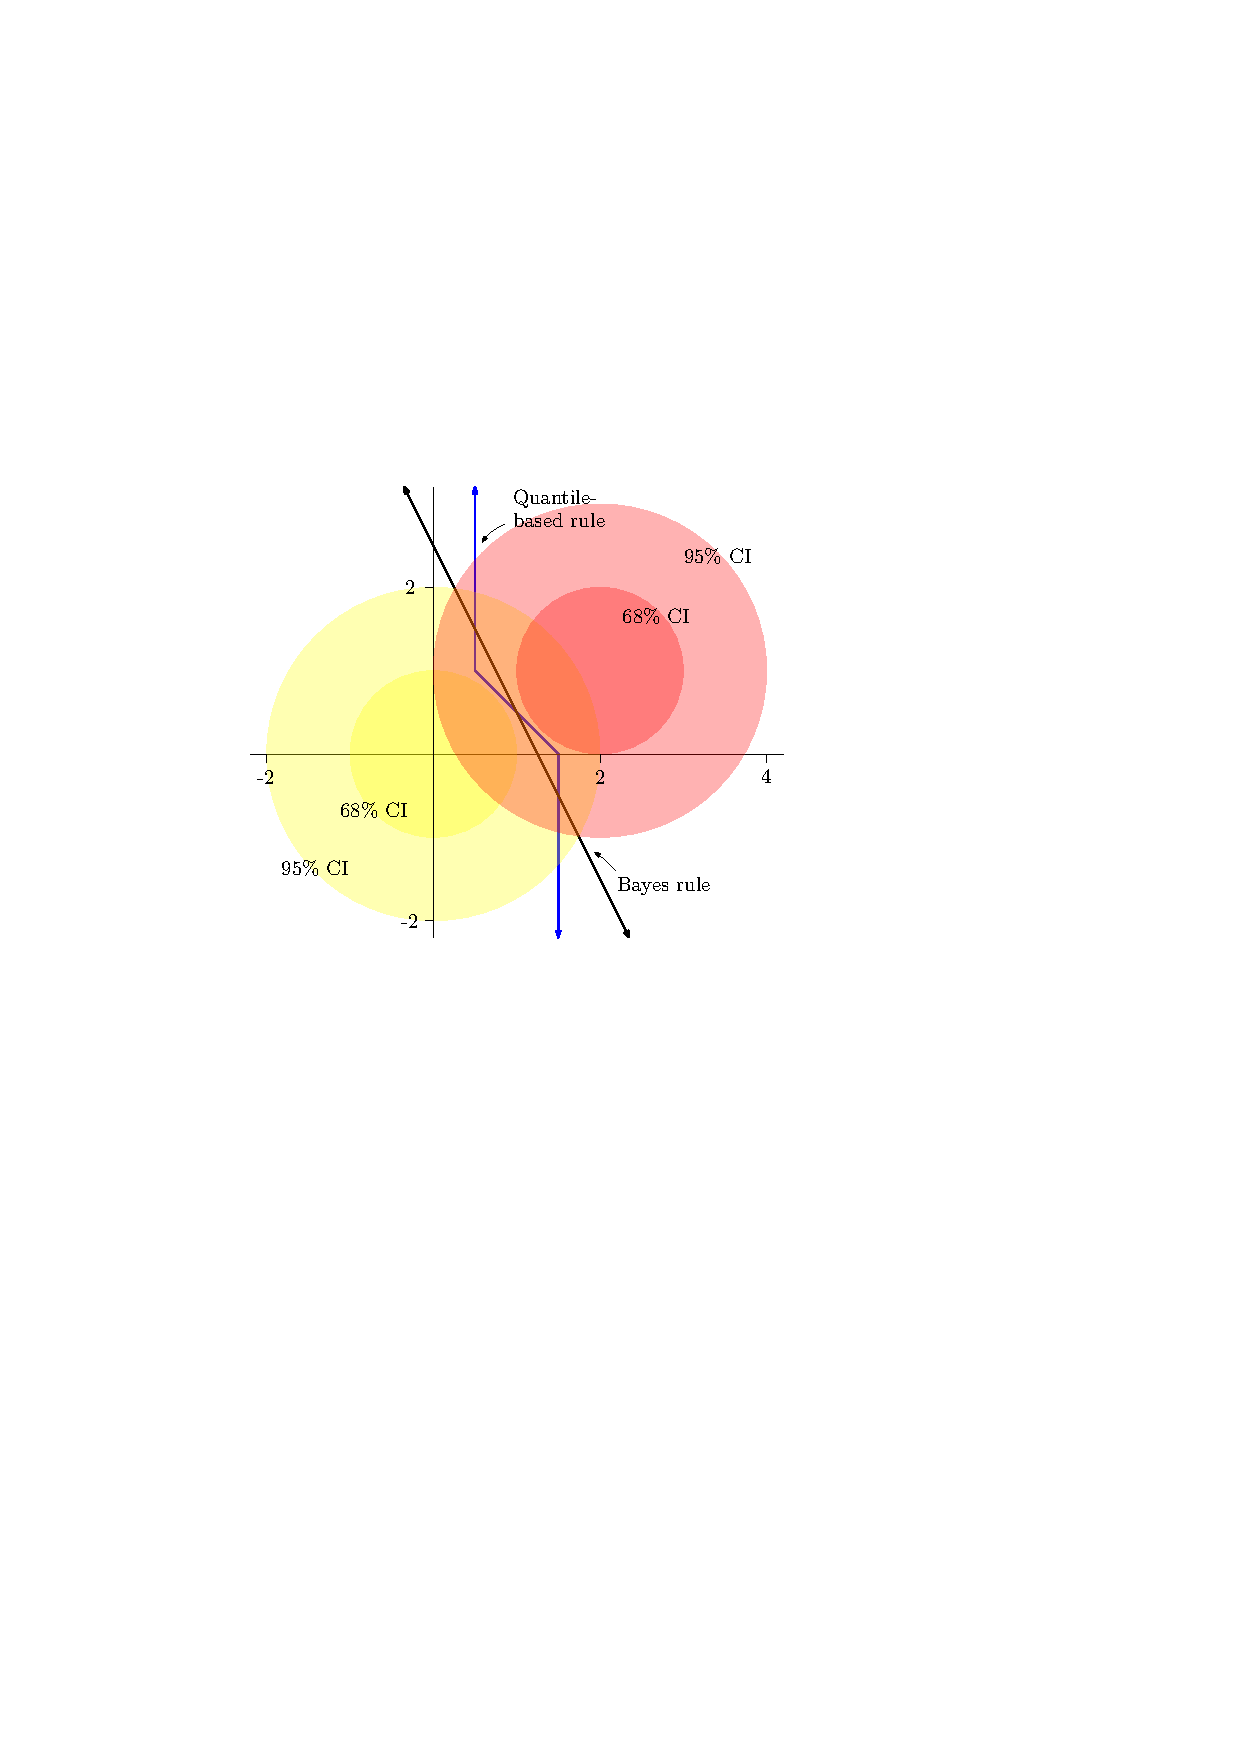
\includegraphics[width=0.96\textwidth]{gauss_ci}
  \end{minipage}
  \begin{minipage}[t]{0.44\linewidth}
    \flushright
    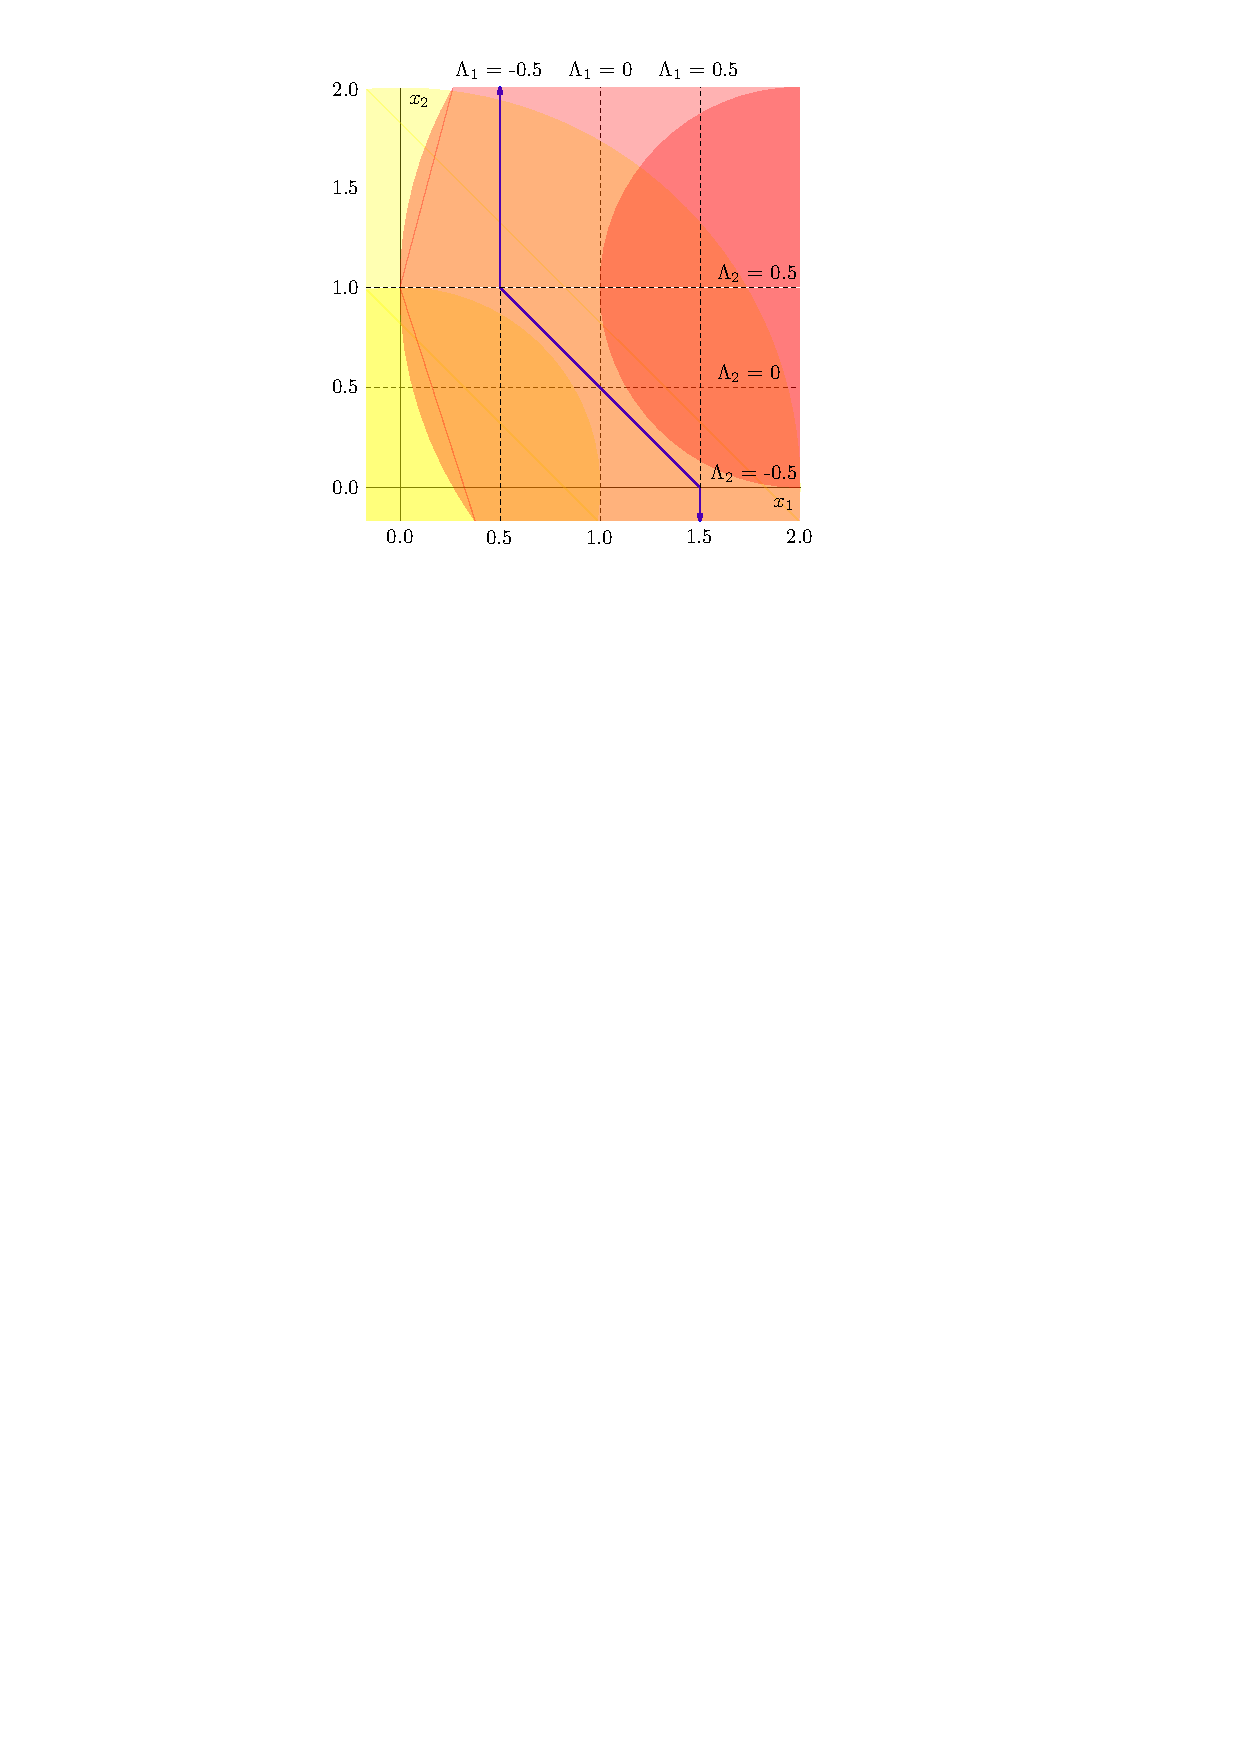
\includegraphics[width=1\textwidth]{gauss_quant_rule}
  \end{minipage}
\end{figure}


% \subsubsection{Classifier examples in two dimensions: Exponentiated Gaussian
%   data}
% \label{sec:classifier-examples-exp-gaussian}

% In a second example, shown as Figure \ref{fig:exponentiated-gaussian}, we
% consider the setting of two location-shifted exponentiated Gaussian
% distributions.  In more detail, if $(W_1, W_2) \sim N(\vec{0}, \vec{I})$, then
% class 0 follows a distribution given by $(e^{W_1},\, e^{W_2})$ and class 1
% follows a distribution given by $(e^{W_1} + 1,\, e^{W_2} + 1)$.  It turns out
% that under this setting, the component-wise Bayes rule decision boundaries are
% given by the location shift, which in this example is 1 for each component.  The
% corresponding quantile level yields within-class quantiles of 0.5 and 1.5 for
% the two classes for each component, so we obtain the decision boundary line
% $\{(x_1, x_2) : x_2 = -x_1 + 2\}$ in the region $[0.5, 1.5]^2$.  Outside of this
% region is a little bit more subtle.  The decision rule boundary lines shown in
% Figure \ref{fig:exponentiated-gaussian} are contingent on the fact that we have
% favorably chosen that tied distances be classified to the correct class
% (i.e. the distribution with the yellow color).  Had we had chosen that the
% tiebreaker had gone in the other direction then the decision rule boundary lines
% outside of the region $[0.5, 1.5]^2$ would switch from going up and right to
% left and down.  This unfavorable tiebreaker policy results in a 2.4\% decrease
% in the composite quantile-based classifiers classification rate.  Otherwise the
% classification rate for the composite quantile-based classifier is 0.71, while
% the classification rate for the Bayes rule classifier is 0.75.

% This setting is
% interesting to consider because although this looks like a difficult case for
% quantile-based classifiers to handle, the classifier actually does really well
% in comparison to competitors in higher dimensions, as is shown in the numerical
% studies.

% \begin{figure}[ht]
%   \caption{Exponentiated Gaussian distributions classifier}
%   \label{fig:exponentiated-gaussian}
%   \centering
%   \vspace{5mm}

%   \begin{minipage}[t]{0.49\linewidth}
%     \flushleft
%     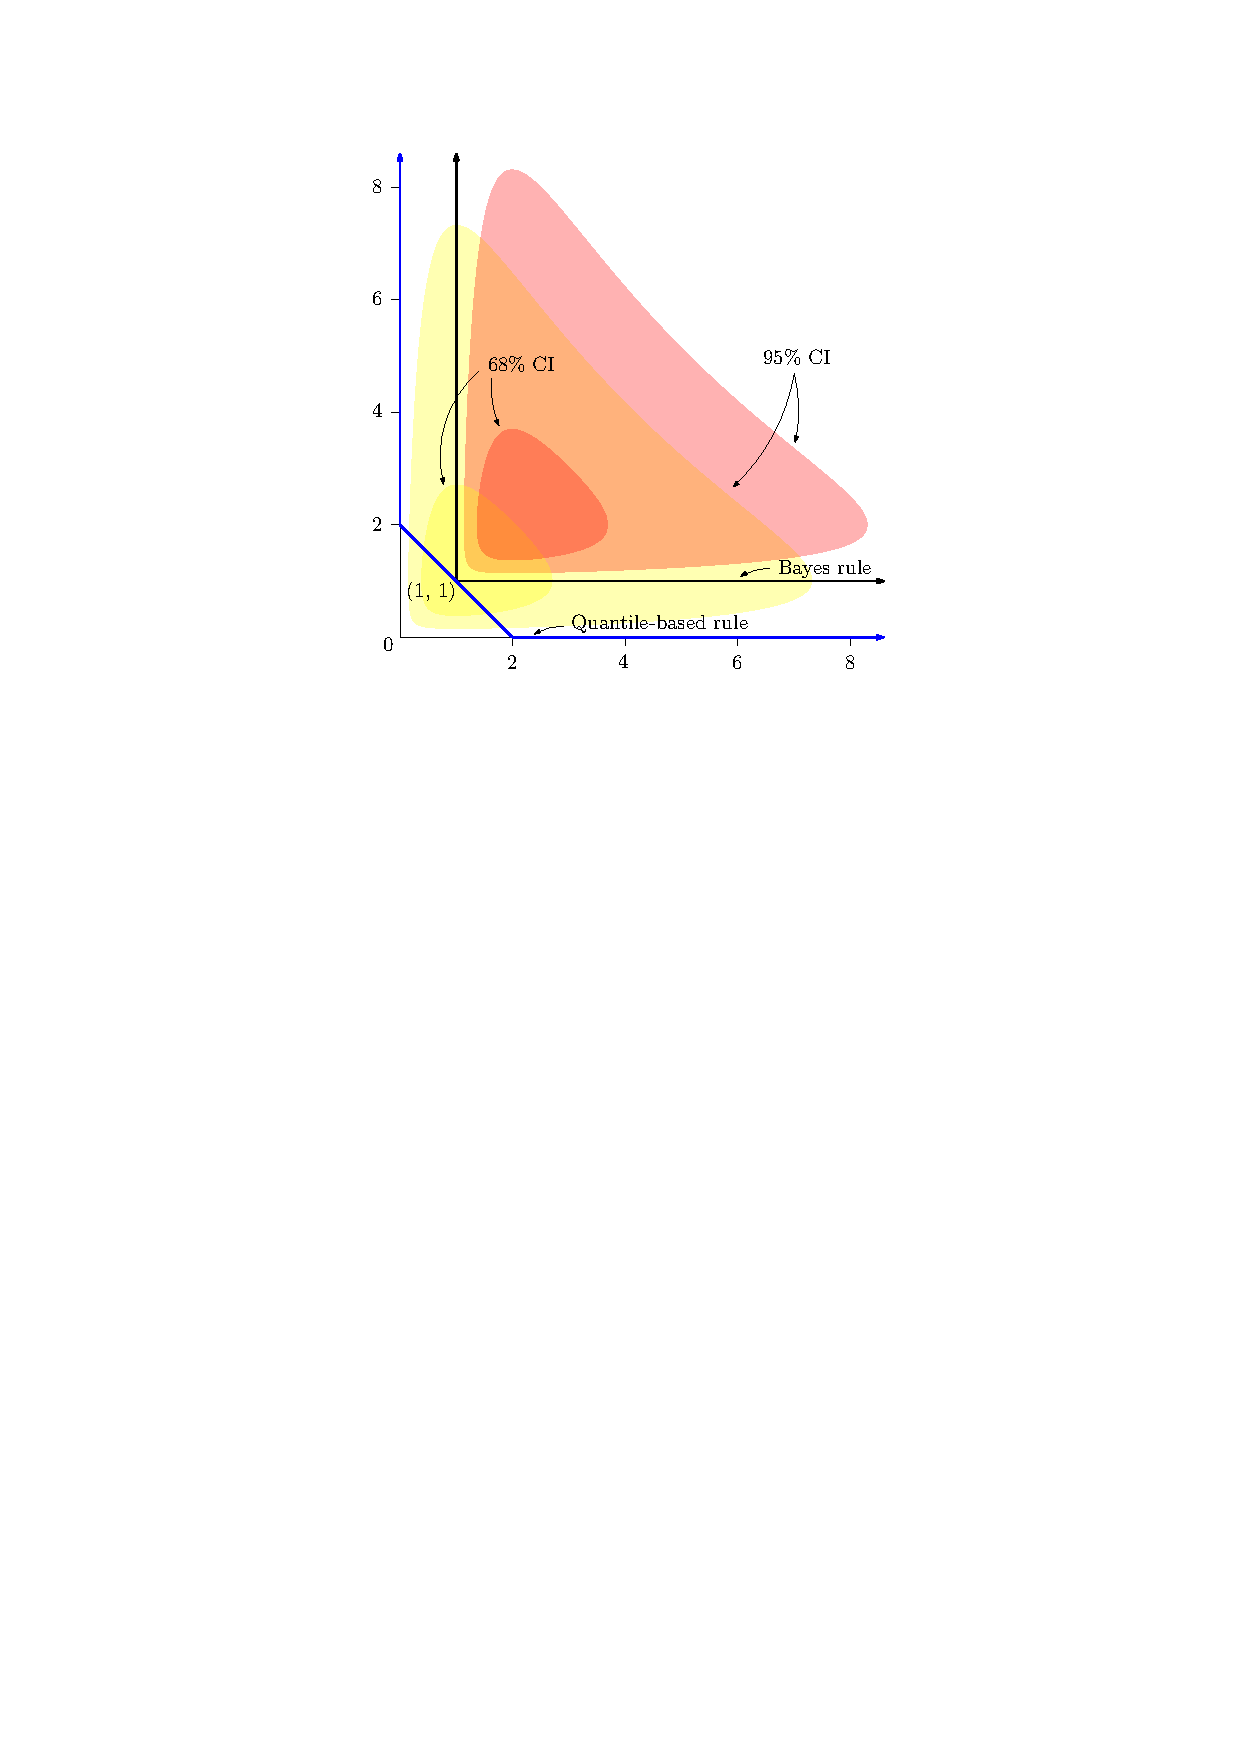
\includegraphics[width=0.95\textwidth]{exp_gauss_ci}
%   \end{minipage}
%   \begin{minipage}[t]{0.49\linewidth}
%     \flushright
%     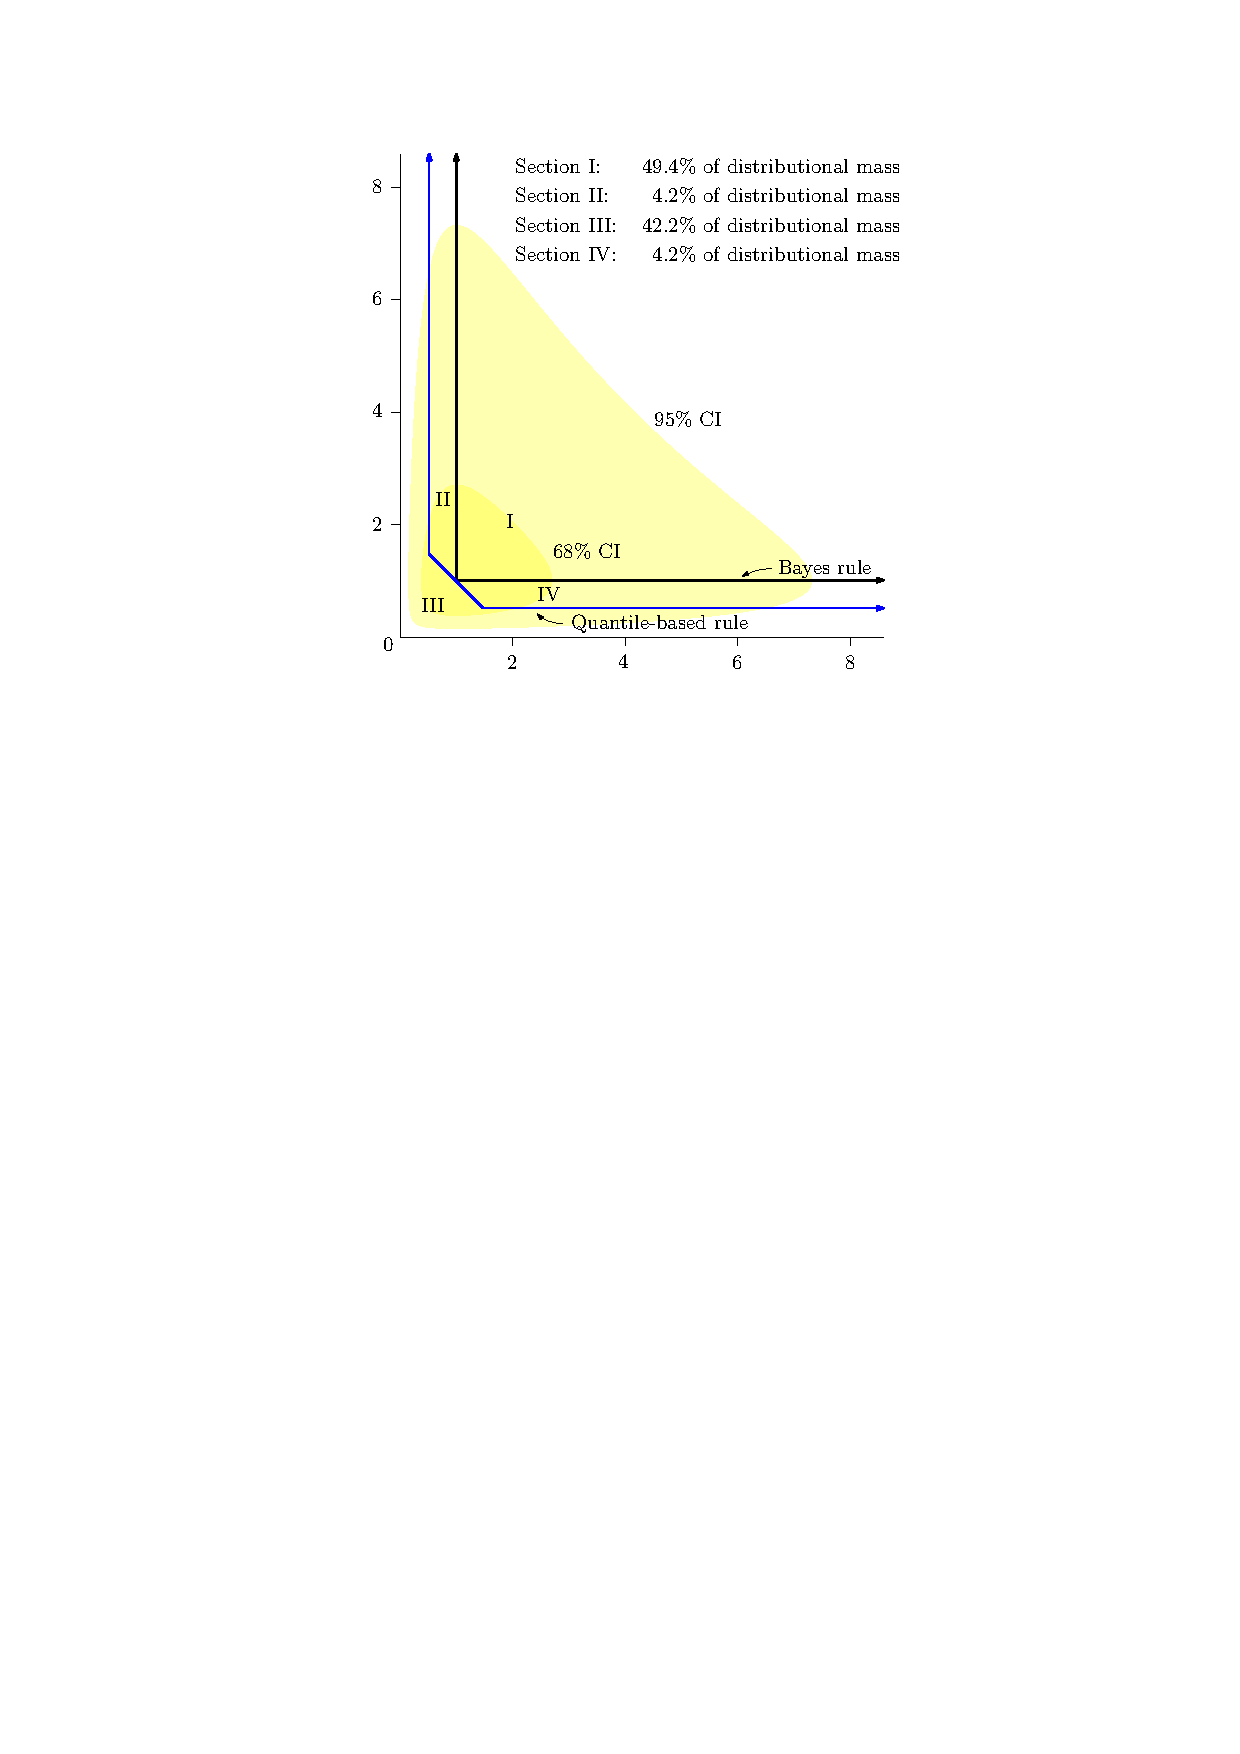
\includegraphics[width=0.95\textwidth]{exp_gauss_rule}
%   \end{minipage}
% \end{figure}




\subsubsection{Classifier examples in two dimensions: beta and gamma distributed data}
\label{sec:beta-gamma-example}

In the following examples we consider settings where the shape of the
component-wise within-class marginal distributions varies across populations.
In the first example, we consider populations where the within-class
distributions follow independent beta distributions, and in the second example
we consider populations where the within-class distributions follow independent
gamma distributions.  The parameters of the beta and gamma distributions were
chosen arbitrarily.  As in the previous example, contour lines denoting 68\% and
95\% percent of the distributional mass for each population are shown.  The
Bayes rule decision boundary is shown as the black line and the composite
quantile-based decision rule boundary is shown as the blue line.  The composite
quantile-based classifiers rule has a classification rate of 0.84 compared to
0.87 for the Bayes rule for the beta distributed data, and a classification rate
of 0.75 compared to 0.76 for the gamma distributed data.

In both examples we see that the Bayes rule decision boundary is nonlinear, so
we can only at best hope to approximate it.  Fortunately, in both examples the
composite quantile-based decision rule boundary follows the Bayes rule decision
boundary well in the higher-density regions of the distributions.  As the Bayes
rule decision boundary moves into low-density distributional regions the
approximation is less accurate due to the form of the composite quantile-based
classifiers.  In our experience this is typical of composite quantile-based
classifiers: the approximation of the Bayes rule is often good at the center of
the data and is less accurate at the edges.

\begin{figure}[ht]
  \caption{Exponentiated Gaussian distributions classifier}
  \label{fig:exponentiated-gaussian}
  \centering
  \vspace{5mm}

  \begin{minipage}[t]{0.49\linewidth} \vspace{0mm}
    \centering
    Beta distributed data \\[2ex]
    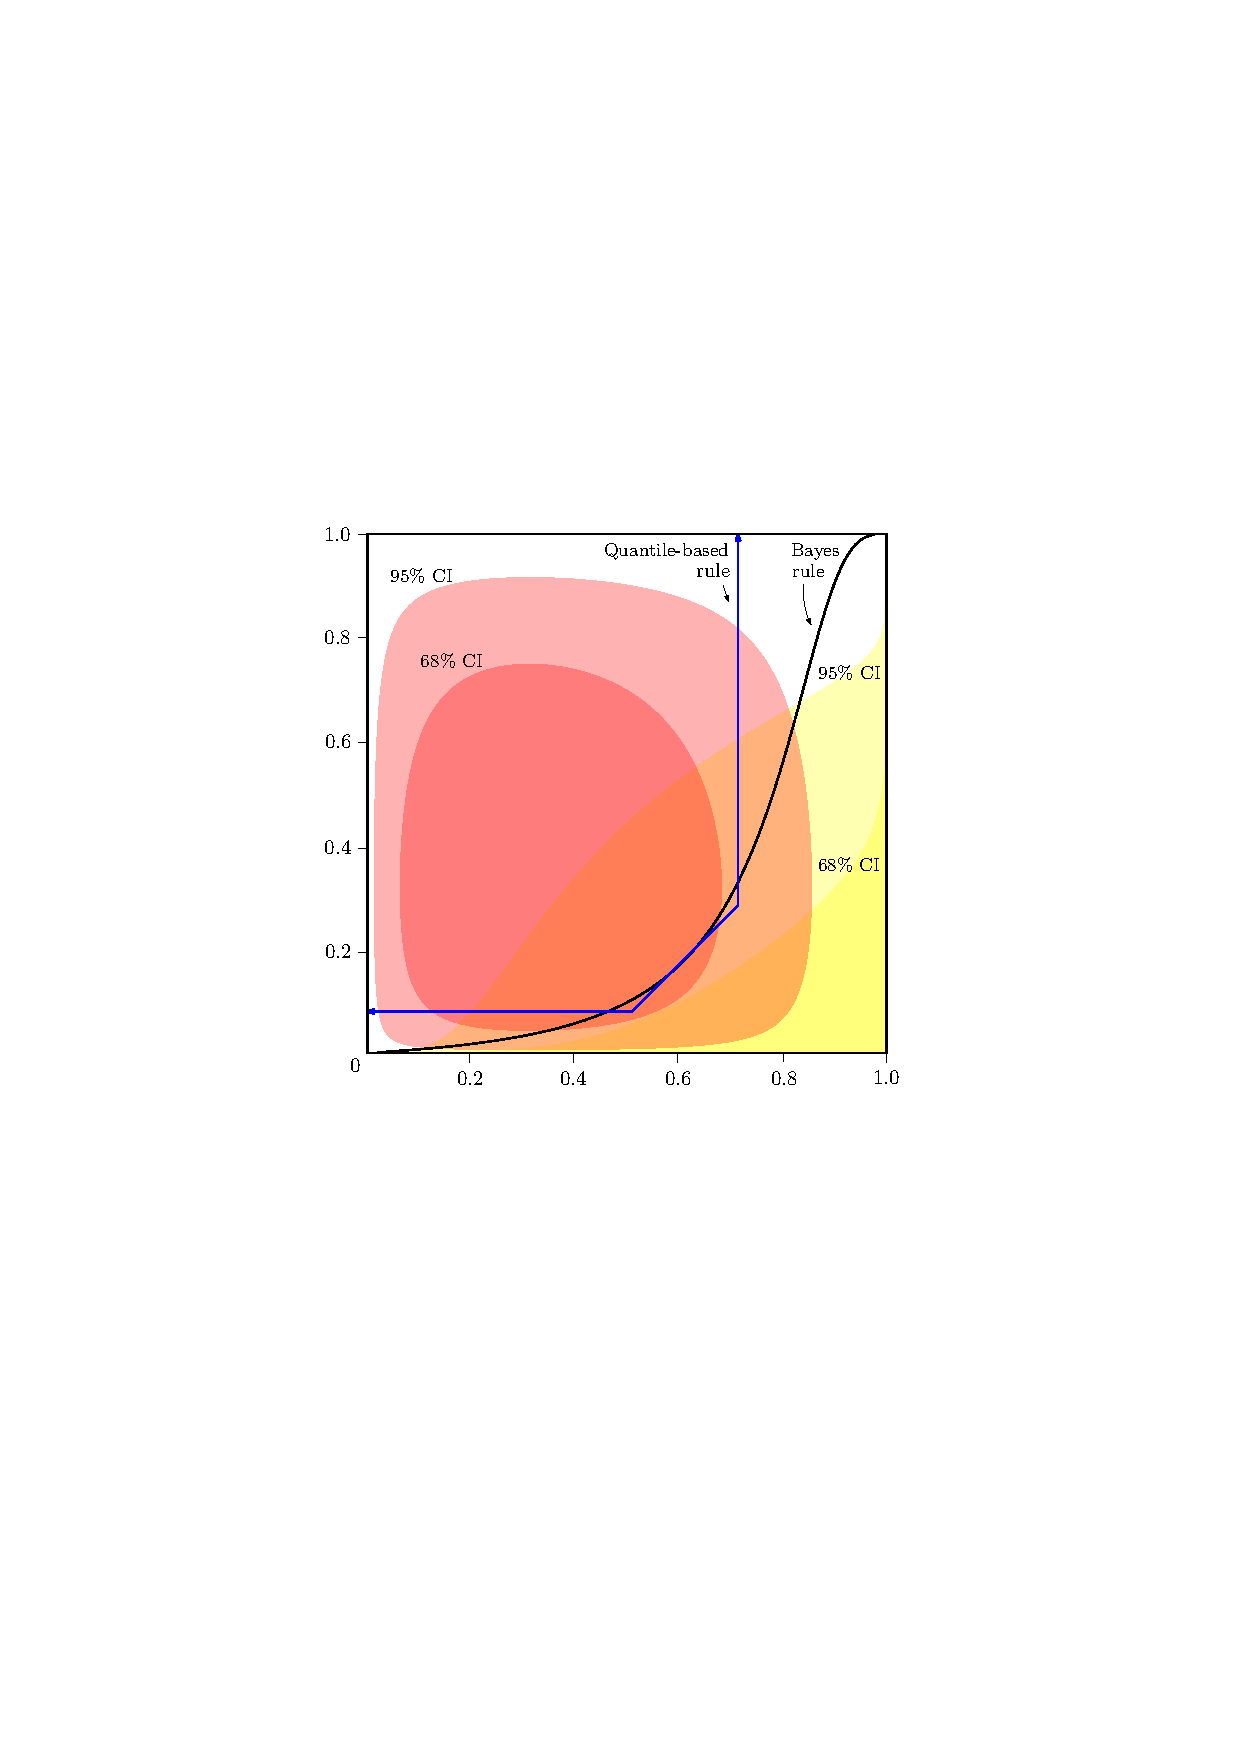
\includegraphics[width=0.975\textwidth]{beta_cqc}
  \end{minipage}
  \begin{minipage}[t]{0.49\linewidth} \vspace{0mm}
    \centering
    Gamma distributed data \\[2ex]
    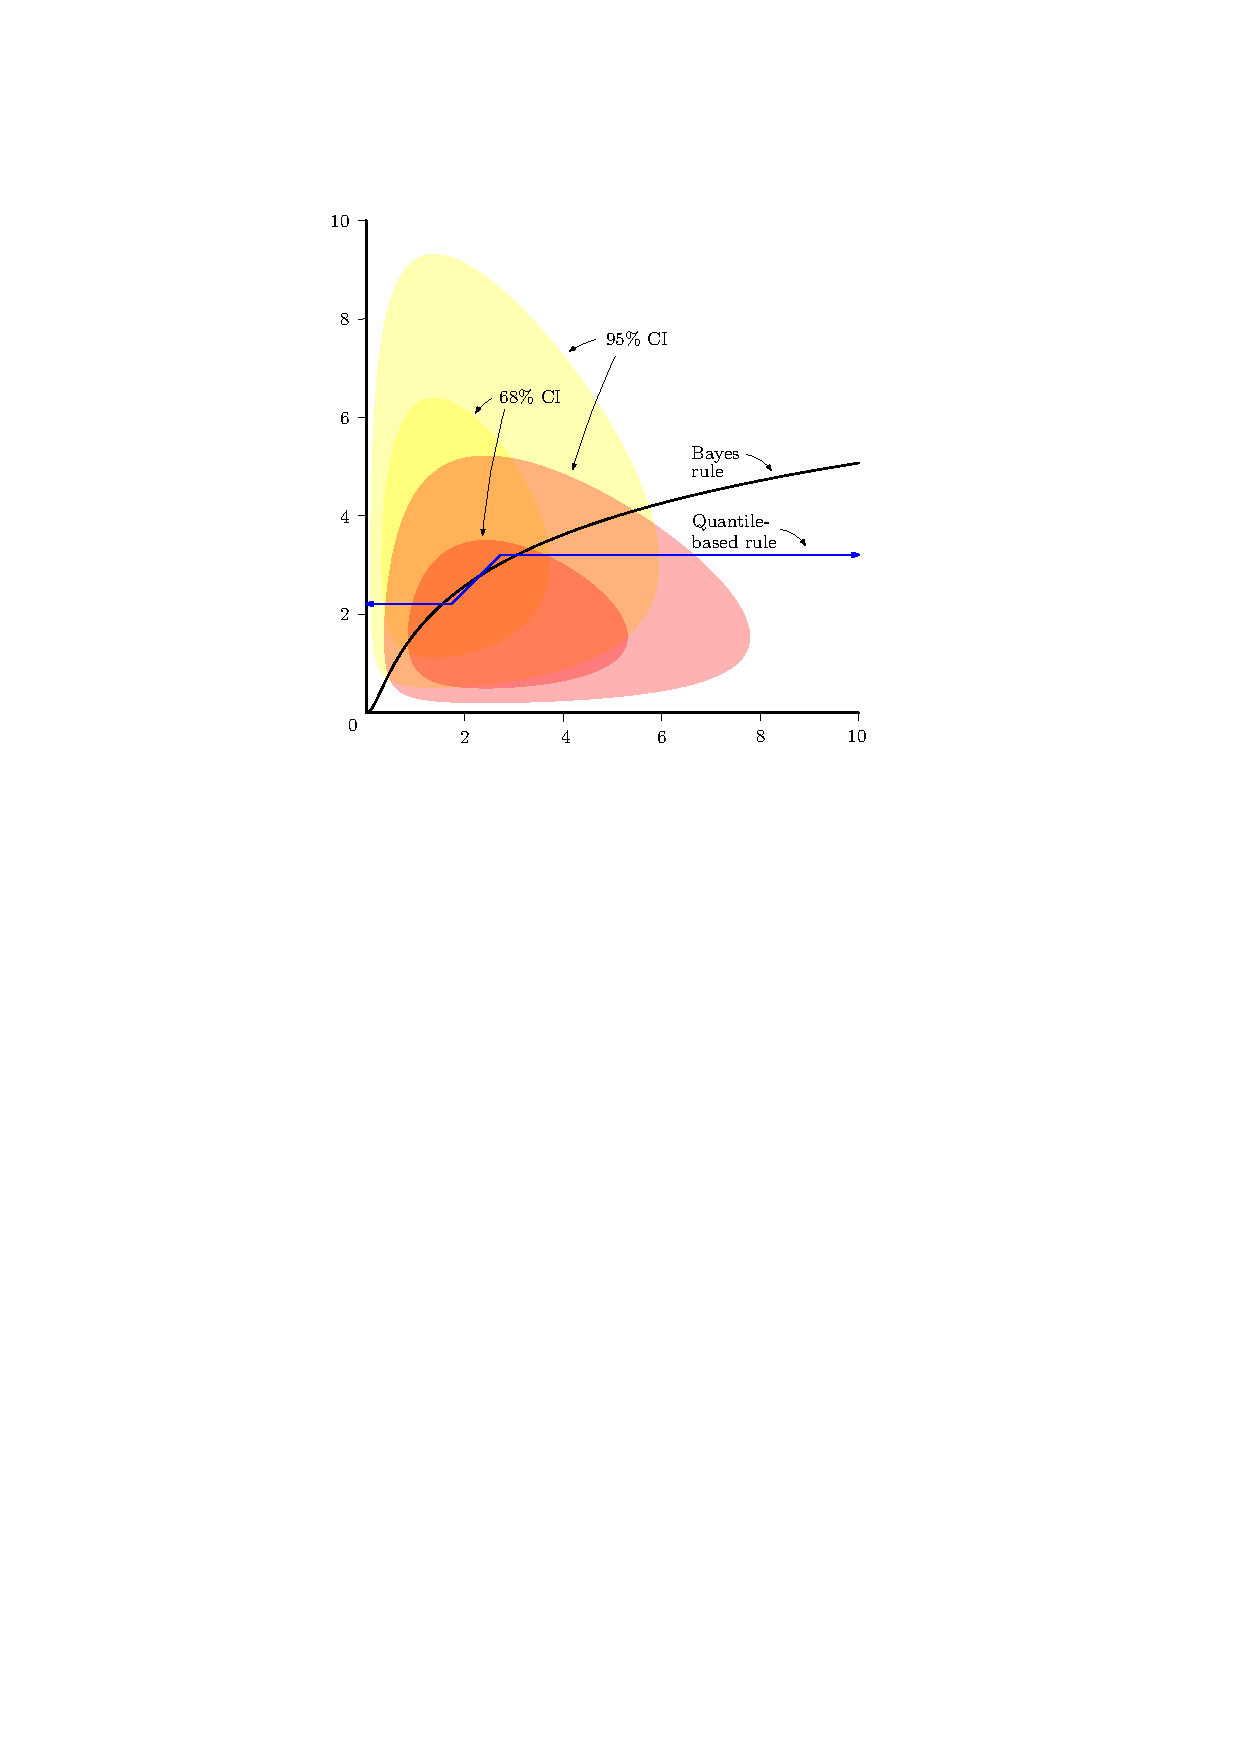
\includegraphics[width=0.975\textwidth]{gamma_cqc}
  \end{minipage}
\end{figure}




\subsubsection{Potential instabilities of composite quantile-based methods}
\label{sec:instabilities}

One potential source of instability of composite quantile-based classifiers is
that the direction of the decision rule boundary lines are dependent on the
magnitude of the difference between the component-wise class quantiles.  This
raises two concerns.  Firstly, changes in scale of the features can
fundamentally affect the classifier by changing which components are part of the
linear systems in the piecewise affine sets.  As a result, when some of the
features in the data are very different in scale to other features then we
recommend some sort of data transformations to try to keep the features at a
similar scale before performing classification.

On the other hand, a second potential source of instability for composite
quantile-based classifiers occurs when the magnitude of the differences between
the within-class quantiles is very similar for two or more features.  When this
is the case, small changes in the within-class quantile estimates can
fundamentally affect the classifier by changing which components are part of the
linear systems in the piecewise affine sets.  On the other hand, when the
within-class quantiles are similar for a given component, this has the effect
that the component contributes very little information to the classifier
aggregate, so that although the form of the classifier may show some instability
the classification rate will typically remain unaffected.  We also expect
averaging the model as discussed in Section \ref{sec:classifier-algorithm} to
help protect against this type of instability.




\subsubsection{Limitations of composite quantile-based classifiers}
\label{sec:limitations}

There are two main limitations of composite quantile-based classifiers that are
evident based upon the form of the classifiers.  The first limitation is that
the classifiers decision rule boundaries are piecewise linear and consequently
can only hope to approximate nonlinear decision rule boundaries.  For some
problems this can result in a loss of efficiency when compared to more flexible
methods.

A second limitation of composite quantile-based classifiers is that there can
only be a single decision rule boundary for any dimension.  Consider an example
where the densities of two populations are perfectly separated into two
concentric circles.  The Bayes rule can perfectly classify this situation, but
any composite quantile-based classifiers decision rule boundary is totally
unable to capture both sides of the inner circle.

We view the limitations of composite quantile-based classifiers as a trade-off
between simplicity of the classifier and its ability to perform well in all
situations.  No single classifier can be expected to perform well in all
settings.  Due to the simple nature of the classifier it is well-suited for
high-dimensional problems, even in the presence of limited data.  However, it is
important to recognize that there are settings for which composite
quantile-based classifiers are ill-suited.




%%% Local Variables:
%%% mode: latex
%%% TeX-master: "cqc_paper"
%%% End:


% folded into multivariate rules
% 
\section{Asymptotic theory}
\label{sec:asymptotic-theory}

\subsection{Consistency of the aggregate quantile classifier}
\label{sec:aggregate-classifier-consistency}

Having established the theoretical optimality of the quantile classifier, we now
consider the consistency of the empirical version.  For the next lemma, we will
need the following assumptions.  Let $\delta$ be a small positive constant.

\begin{enumerate}[label=\emph{Assumption \arabic*.}, align=left]
\item $F_{ij}^{-1}$ is a continuous function of
  $\theta,~ i=0,1,~ j=1, \dots, p$.
\item $\prob\Big(
  \sum_{j=1}^p \Lambda_j (Z_j, \theta_j) = 0
  \Big) = 0$ for all
  $\theta \in [\delta, 1 - \delta]$.
\item There is a unique $\tilde{\theta}_j$ that satisfies
  $\tilde{\theta} = \argmax_{\theta \in T} \Psi_j(\theta), j = 1, \dots, p$.
\end{enumerate}
Let $\tilde{\theta}_j$ denote the unique maximizer of
$\Psi_j(\theta),~ j=1, \dots, p$, and further denote
$\tilde{\vec{\theta}} = \Big( \tilde{\theta}_1, \dots,
\tilde{\theta}_P \Big)$.
\vspace{5mm}

\begin{theorem}
  Under assumptions 1-3 it follows that
  $\Psi(\hat{\vec{\theta}}_n) \convp \Psi(\tilde{\vec{\theta}})$.
\end{theorem}

\begin{proof}
  The following upper bound on the difference between the component-wise
  quantile distances was established in the proof of Theorem 1 in Hennig and
  Viroli (2016).  For $z \in \mathbb{R}$ and
  $\theta, \theta^{\prime} \in (0, 1)$ then
  \begin{equation}
    \label{eq:quantile-distance-ubnd}
    \big| \Phi_{ij}(z, \theta) - \Phi_{ij}(z, \theta^{\prime}) \big|
    \leq |z|\, | \theta - \theta^{\prime} | +
    4 | F_{ij}^{-1}(\theta) - F_{ij}^{-1}(\theta^{\prime}) |,
    \hspace{5mm} i = 1, 2,~ j = 1, \dots, p
  \end{equation}
  Since $F_{ij}^{-1}$ is continuous by assumption, it follows that for arbitrary
  fixed $z$, $\Phi_{ij}(z, \theta)$ is continuous in $\theta$ for every
  $\{i, j\}$.  This in turn implies that for arbitrary fixed $\vec{z}$,
  $\Lambda(\vec{z}, \vec{\theta})$ is also continuous in $\vec{\theta}$, since
  $\Lambda$ is just the sum of the differences of the
  $\Phi_{ij}(z_j, \theta_j)$'s.  Then we observe that
  \begin{align}
    \label{eq:multivariate-phi-continuity}
    \begin{split}
      \limtheta \Psi(\vec{\theta})
      & = \limtheta \left\{
        \pi_0 \int \ind\Big( \Lambda(\vec{z}, \vec{\theta}) > 0 \Big)\, dP_0(\vec{z}) +
        \pi_1 \int \ind\Big(\Lambda(\vec{z}, \vec{\theta}) \leq 0 \Big)\, dP_1(\vec{z})
      \right\} \\[1ex]
      & = \pi_0 \int \limtheta \ind\Big( \Lambda(\vec{z}, \vec{\theta}) > 0 \Big)\, dP_0(\vec{z})
      + \pi_1 \int \limtheta \ind\Big(\Lambda(\vec{z}, \vec{\theta}) \leq 0 \Big)\, dP_1(\vec{z})
      \\[1ex]
      & = \pi_0 \int \ind \Big( \limtheta \Lambda(\vec{z}, \vec{\theta}) > 0 \Big)\, dP_0(\vec{z})
      + \pi_1 \int \ind \Big( \limtheta \Lambda(\vec{z}, \vec{\theta}) \leq 0 \Big)\, dP_1(\vec{z})
      \\[1ex]
      & = \pi_0 \int \ind \Big( \Lambda(\vec{z}, \vec{\theta}^{*}) > 0 \Big)\, dP_0(\vec{z})
      + \pi_1 \int \ind \Big( \Lambda(\vec{z}, \vec{\theta}^{*}) \leq 0 \Big)\, dP_1(\vec{z})
      \\[1ex]
      & = \Psi(\vec{\theta}^{*})
    \end{split}
  \end{align}
  The justification for bringing the limit inside of the integral is due to the
  dominated convergence theorem.  The justification for bringing the limit
  inside of the indicator function is that the indicator function is continuous
  everywhere except at 0, which by Assumption 2 occurs with probability 0, and
  hence does not change the value of the integral.  This result establishes that
  $\Psi$ is continuous in $\vec{\theta}$.

  It was established in Lemma \ref{lem:univariate-consistency} that
  $\hat{\theta}_{jn} \convp \tilde{\theta}_j$, so by Slutsky's theorem
  it follows that $\hat{\vec{\theta}}_n \convp \tilde{\vec{\theta}}$.
  Then by the result obtained in equation
  (\ref{eq:multivariate-phi-continuity}), a second application of Slutsky's
  theorem yields
  $\Psi(\hat{\vec{\theta}}_n) \convp \Psi(\tilde{\vec{\theta}})$.
\end{proof}








%%% Local Variables:
%%% mode: latex
%%% TeX-master: "cqc_paper"
%%% End:




\section{Numerical results}
\label{sec:numerical-results}


\subsection{Simulation studies}
\label{sec:simulation-studies}

In this section we consider the performance of the composite quantile-based
classifiers compared to other related and popular classification methods.  A
total number of 8 scenarios are considered.  Within each scenario, we consider
combinations of sample sizes $n = 500, 250, 50$ and data dimension
$p = 50, 250, 500$.  Here $n$ is taken to be the total number of samples and in
every setting we consider equal numbers of observations for each class, so that
the number of samples from each class is $n / 2$.  Additionally, although the
number of features varies for different simulations, the number of
discriminatory features remains fixed at 50 throughout all of the simulations.
That is to say, that for every simulation there are 50 features such that the
distribution of the features varies across the classes, and the remaining
features (if any) are noise variables drawn from the same distribution for each
class.  The noise variables were drawn independently of each other from a
Gaussian distribution for each scenario.


\subsubsection{Simulated data scenarios}
\label{sec:simulated-data-scenarios}

Consider the following framework for each of the scenarios.  Let
$\vec{Z} = (Z_1, \dots, Z_p) \sim N(\vec{0},\, \vec{\Sigma})$, and let
$\vec{V}_i = (V_{i1}, \dots, V_{ip})$ and $\vec{W}_i = (W_{i1}, \dots, W_{ip})$
be observations from two populations, $i = 1, \dots, n / 2$, and where the
$\vec{V}_i$ and $\vec{W}_i$ are all mutually independent.  There are two choices
of covariance matrices considered for $\vec{\Sigma}$.  In some scenarios we
consider independent data where the covariance matrix is the identity matrix,
and in other scenarios we consider the correlated data with an autoregressive
lag 1 covariance matrix (abbreviated as AR1).  The AR1 matrix is specified with
variance parameters identically 1 on the diagonal, and correlation parameter
0.8.  In the interest of continuity, the scenarios are designed to be similar to
the simulation settings presented in \cite{hennig2016}.

In the first and second scenarios, we consider two classes each with features
drawn from a multivariate Gaussian distribution and with one class given a
location shift.  In more detail then, for each feature we consider
$V_{ij} \sim Z_j$ and $W_{ij} \sim Z_j + 0.35$.  In the first scenario we
consider uncorrelated data for the underlying Gaussian distribution, and in the
second scenario we consider autoregressive correlation.

In the third and fourth scenarios, we consider highly skewed data by
exponentiating the components of a Gaussian distribution.  That is to say that
$V_{ij} \sim \exp(Z_j)$ and $W_{ij} \sim \exp(Z_j) + 0.35$.  In the third
scenario we consider uncorrelated data for the underlying Gaussian distribution,
and in the fourth scenario we consider autoregressive correlation.

In the fifth and sixth scenarios we consider different distributions for each of
5 blocks of features.  In more detail, the data is sampled from a Gaussian
distribution and then $p$ features are evenly split into 5 blocks and the
following transformations performed to each block: (i) $V_{ij} \sim Z_j$ and
$W_{ij} \sim Z_j + 0.2$, (ii) $V_{ij} \sim \exp(Z_j)$ and
$W_{ij} \sim \exp(Z_j) + 0.2$, (iii) $V_{ij} \sim \log |Z_j|$ and
$W_{ij} \sim \log |Z_j| + 0.1$, (iv) $V_{ij} \sim Z_j^2$ and
$W_{ij} \sim Z_j^2 + 0.2$, and (v) $V_{ij} \sim |Z_j|^{1/2}$ and
$W_{ij} \sim |Z_j|^{1/2} + 0.1$.  In the fifth scenario we consider uncorrelated
data for the underlying Gaussian distribution, and in the sixth scenario we
consider autoregressive correlation.

In the seventh and eight scenarios, we considered data with different
distributional shapes within each feature.  In the seventh scenario we
considered data with independent beta distributed features and in the eight
scenario we considered data with independent gamma distributed features.  The
beta distribution parameters were sampled as follows.  Two shape parameters were
sampled for each feature each from a $\mathit{unif}(0.1, 3)$ and
$\mathit{unif}(0.5, 3)$ distribution for each shape parameter, respectively.
Then for each class and feature, each parameter was transformed by taking the
absolute value of some additive Gaussian random noise.  So for example, suppose
that $\alpha_j$ and $\beta_j$ are the shape parameters drawn for the $j$-th
feature.  Then for each class the distributional parameters are each sampled
from $|\alpha_j + N(0, \sigma_j^2)|$ and $|\beta_j + N(0, \sigma_j^2)|$
distributions.  $\sigma_1, \dots, \sigma_{50}$ were given by a fixed sequence
each with values between 0.05 and 0.20.  Once the shape parameters were sampled,
the same parameters were used for every replicate and every simulation study.
Finally, the gamma distribution parameters in the eight scenario were sampled in
essentially the same manner.


\subsubsection{Hybrid CQC and quantile-based classifiers}
\label{sec:hybid-cqc}

One disadvantage of the CQC approach is that the data is partitioned into two
parts: one for selecting quantile levels and estimating quantiles, and the other
for training the linear combination coefficients, so that each of these tasks is
performed using only a subset of the data.  When data is abundant, there is
typically not a great loss of efficiency when performing these tasks as compared
to using all of the available data.  However, when data is limited, losing a
portion of the data can result in a large loss of efficiency.  As a concrete
example, suppose $n = 50$ and we split the data into two equal parts.  Then
estimating the within-class quantiles is limited to 25 points so that the
quantiles are estimated for at least one class with no more than 12 data points
- a big difference to estimating the quantiles from 25 data points.  When data
is limited as in this example, we find that CQC can suffer from instability in
the choice of quantile levels.  As a result, we suggest using the quantile
levels as selected by the quantile-based classifiers method and then applying
the linear combination step on the transformed variables as in the usual CQC
method.  This has the result in choosing quantile levels that are far more
stable at the cost of some flexibility.  Our suggestion is that when data is
relatively small, say less than 100, to perform cross-validation with the
regular CQC and hybrid approach to select the better model.  It is noted in the
discussion of the simulations whenever the hybrid approach is used.


\subsubsection{Classifier implementations and settings}
\label{sec:classifier-implementations}

We compared the misclassification rate from the composite quantile-based
classifiers model with that of nine other classification methods: quantile-based
classifiers \cite{hennig2016}, FANS \cite{fan2016}, penalized linear regression
($\ell_1$ penalty) \cite{park2007}, support vector machine (radial kernel)
\cite{cortes1995}, k-nearest neighbor \cite{cover1967}, naive Bayes
\cite{hastie2009}, nearest shrunken centroids \cite{tibshirani2002}, penalized
LDA \cite{witten2011}, and decision trees \cite{breiman1984}.  

The composite quantiles-based classifier is implemented using the \r/
programming language; the source code is available from the authors upon
request.  Quantile-based methods is implemented as the \r/ package
\texttt{quantileDA}.  There are several methods of quantifying distributional
skew provided by the package; we used the default Galton skewness measure.  FANS
is implemented as \matlab/ \cite{matlab} source code and is available upon
request by the authors of \cite{fan2016}.  Results from both the FANS method and
FANS2 method are shown since FANS2 is similar to the augmented version of
composite quantile-based classifiers.  Penalized linear regression is
implemented as the \r/ package \texttt{glmnet} and uses the $\ell_1$ penalty
with 10-fold cross validation to select the penalty parameter.  Support vector
machine is implemented in the \r/ package \texttt{e1071} through the C++ library
\texttt{libsvm}.  The tuning parameters for each simulation were selected by
using the function \texttt{tune.svm} over the kernel coefficient parameter from
among $\{0.001, 0.01, 0.1, 1, 2\}$, and constraints violation cost from among
$\{1, 2, 4, 8, 16\}$.  k-nearest neighbors is implemented in the \r/ package
\texttt{class} and uses leave-one-out cross validation to choose the number of
neighbors considered from among $\{1, \dots, 9\}$.  Naive Bayes is implemented
in the \r/ package \texttt{e1071}.  Nearest shrunken centroids is implemented as
the \r/ package \texttt{pamr} with 10-fold cross validation used to select the
threshold parameter.  The version of penalized linear discriminant analysis
compared in the simulation studies is that proposed in \cite{witten2011}, and is
implemented as the \r/ package \texttt{PenalizedLDA} using 6-fold cross
validation and 1 discriminant vector.  Decision trees is implemented as the \r/
package \texttt{rpart}.  All packages used in the numerical analysis are
available from the Comprehensive \r/ Archive Network.


\subsubsection{Simulation results}
\label{sec:simulation-results}

The classifer proposed in this paper is abbreviated as CQC.  Results for the
second variant of composite quantile-based classifiers are also shown and are
abbreviated as CQC augmented.  This is the variant where transformed quantile
distances data is augmented by the original data when constructing the decision
rule.

Simulation results for the Gaussian setting are shown in Table
\ref{tab:gauss-corr0} and Table \ref{tab:gauss-corr08}.  We would expect
composite quantile-based classifiers to be suboptimal in this setting compared
to LDA and similar classifiers since they do not make use of the distributional
information, and are interested in the magnitude of the loss of efficiency.  One
thing to notice is that the augmented version of CQC performs better nearly
everywhere as compared to the non-augmented version.  This is to be expected
since the Bayes rule decision boundary is linear in the original features, and
is also the case for FANS2 as compared to FANS.  In this setting, nearest
shrunken centroids and penalized LDA show the best performance.  When $n$ is
large compared to $p$, marginal quantile-based classifiers perform reasonably
well, although performance deteriorates relative to other methods when
conditions are less ideal.

Simulation results for the exponentiated Gaussian setting are shown in Table
\ref{tab:exp-gauss-corr0} and Table \ref{tab:exp-gauss-corr08}.  As we saw in
Section \ref{sec:classifier-examples}, that in this setting quantile-based
classifiers are nearly optimal and this is borne out in the simulation study
results.  CQC performs well also, although never as well as quantile-based
classifiers.  We see this as being due to several reasons.  Firstly,
quantile-based classifiers composite quantile-based classifiers sacrifice part
of the data set in order to train the linear combination coefficients; this has
the effect of reducing the sample size to both choose good quantile levels and
to estimate the within-class quantiles.  Secondly, since the optimal quantile
level is the same for every quantile, quantile-based classifiers is able to
borrow information across all of the features to estimate the optimal quantile
level, while composite quantile-based classifiers selects the quantile level one
feature at-a-time.  Thirdly, the freedom to select linear combination
coefficients for the composite quantile-based classifiers method can result in
additional variation.  These points highlight the trade-off between the two
methods.  When the optimal quantile levels and discriminatory information are
the same across the components then quantile-based classifiers perform better
than CQC, and when this is not the case then CQC may perform better in some
settings.

Simulation results for the block transformed Gaussian setting are shown in Table
\ref{tab:block-transformed-corr0} and Table \ref{tab:block-transformed-corr08}.
In contrast to scenarios 1-4, in this setting the optimal quantile levels and
discriminatory information vary across the components, and in this setting CQC
typically performs better than quantile-based classifiers.  FANS and decision
trees are the other best-performing classifiers in this scenario.  The inclusion
of decision trees suggests that there are some relatively discriminative
features.  When the quantity of the training data decreases to $n = 50$ we see a
sharp rise in the misclassification rates for all methods.  It is in this
setting that the hybrid CQC and quantile-based classifiers do well.  For
example, when $n = 50$ and $p = 500$ with uncorrelated data, using the hybrid
approach reduces the misclassification rate from 0.351 to 0.215.  Both CQC and
quantile-based classifiers perform well in this setting compared to other
methods.  We attribute this in part to the relative simplicity of the models in
this data-sparse setting.  Additionally, the reason that the hybrid approach
works well here is that we may have a number of relatively discriminative
features that the quantile-based methods approach of selecting quantile levels
can effectively key in on, and then the additional linear combination step can
help to deal with some of the differences in scale and discriminatory power
between the blocks.

Simulation results for the beta distributed and gamma distributed data settings
are shown in Table \ref{tab:block-transformed-corr0} and Table
\ref{tab:block-transformed-corr08}.  In the case of the beta distributed data,
CQC and decision trees performed the best.  We see this as a sign of a few
features having some degree of separability across the two classes.  In this
setting where the optimal quantile level varies across all of the features, we
see that CQC having more flexibility to select quantile levels results in better
performance as compared to quantile-based classifiers.  We see similar results
for the gamma distributed data, although in this case quantile-based classifiers
perform about as well as CQC.  We see this as suggesting that there happen to be
a number of features with similar optimal quantile levels that quantile-based
classifiers can select to achieve similar performance as the more flexible
approach.




\subsection{Real data study}
\label{sec:real-data-study}

For a real data study, we considered a spam data with a total of 4,601
observations and 57 features.  The attributes are, for example, the percentage
of specific words or phrases in the email, the average and maximum run lengths
of uppercase letters, and the total number of uppercase letters.  The proportion
of data used to train the methods is varied from 5\% to 80\%.  We see that for
this data set, CQC performs at least as well as the best at every level, with
SVM the next best competitor.



\subsection{Real data considerations}

In practice, one often encounters data that has variables with both continuous
as well as categorical data.  In problems such as these categorical data is
typically reformulated into so-called dummy-coded variables.  However, the
quantile-based classifier is inherently ill-conditioned to handle such data.
When categorical variables are present in the data, we propose including them in
the classifier as untransformed dummy-coded variables.

A second type of data can also cause problems:  one where the data is a mixture
of point masses as well as continuous data.  As an example, consider univariate
data where the the quantiles of the underlying populations are given as follows.
\begin{center}
  \begin{tabular}{lrrrrrrrrrrr}
    \toprule
    & \multicolumn{11}{c}{\underline{Quantile levels}} \\
    & 0.89 & 0.90 & 0.91 & 0.92 & 0.93 & 0.94 & 0.95 & 0.96 & 0.97 & 0.98 & 0.99 \\
    \midrule
    Class 0 & 0.00 & 0.02 & 0.14 & 0.23 & 0.33 & 0.42 & 0.55 & 0.68 & 0.87 & 1.05 & 1.41 \\
    Class 1 & 0.00 & 0.00 & 0.00 & 0.00 & 0.00 & 0.00 & 0.00 & 0.06 & 0.08 & 0.18 & 0.20 \\
    \bottomrule
  \end{tabular}
\end{center}
This example raises the question as to what the quantile distances would be for
a fixed choice of quantile level.  Suppose first that we consider a quantile
level with nonzero quantiles for both classes, say 0.97.  In this case, the
quantile distances for the data in class 0 with value 0 than the data quantile
distances for the data in class 1 with value 0.  As a result, the quantile-based
data will have spuriously introduced differences in the data for 90\% of the
data, when in fact there is no discriminative data in those quantiles.
Conversely, suppose now that we select a quantile level with quantiles for both
classes with value 0.  Doing so has the effect of simply multiplying the nonzero
values in the data by a constant factor.  While this is less disastrous then the
previous scenario, we are not using the quantile-based data approach consistent
with the rest of the paper.

What we propose to do for such a scenario is the following.  When mixture data
such as the example given above is present for a variable, we try to separate
the parts of the data that belong to the point mass contribution to the mixture,
and those that belong to the continuous part of the mixture.  Then for the point
mass data, we create a categorical variable that includes a reference category
for the continuous part of the data, and for the continuous part we perform the
quantile-based classification using only the reduced subset of the data.




% Gaussian data ----------------------------------------------------------------

\begin{table}[p]
  \centering
  Gaussian data \\
  Correlation coefficient = 0 \\[2ex]
  \begin{adjustbox}{max size={\textwidth}{10cm}}
    \begin{tabular}{l@{\extracolsep{15mm}}rrr}
      
      \hline
      & $n=500$ & $n=250$ & $n=50$ \\ 
      \hline
      & $p = 50$ \\
      \hline

      CQC & 0.160 (0.01) & 0.198 (0.02) & 0.286 (0.03) \\ 
      CQC augmented & 0.138 (0.01) & 0.161 (0.02) & 0.263 (0.05) \\
      Quantile-based classifiers & 0.164 (0.01) & 0.186 (0.02) & 0.282 (0.04) \\
      FANS  & 0.189 (0.02) & 0.254 (0.03) & 0.430 (0.04) \\
      FANS2 & 0.141 (0.01) & 0.176 (0.02) & 0.379 (0.07) \\
      Penalized logistic regression & 0.131 (0.01) & 0.161 (0.01) & 0.274 (0.05) \\ 
      Support vector machine & 0.118 (0.01) & 0.129 (0.01) & 0.165 (0.02) \\ 
      k-nearest neighbor & 0.193 (0.01) & 0.214 (0.02) & 0.276 (0.04) \\ 
      Naive Bayes & 0.122 (0.01) & 0.139 (0.01) & 0.213 (0.03) \\ 
      Nearest shrunken centroids & 0.114 (0.01) & 0.126 (0.01) & 0.170 (0.04) \\ 
      Penalized LDA & 0.116 (0.01) & 0.126 (0.01) & 0.161 (0.02) \\ 
      Decision trees & 0.380 (0.01) & 0.388 (0.02) & 0.435 (0.02) \\ [2ex]

      \hline
      & $p = 250$ \\
      \hline

      CQC & 0.196 (0.02) & 0.243 (0.02) & 0.391 (0.03) \\ 
      CQC augmented & 0.158 (0.01) & 0.199 (0.02) & 0.355 (0.03) \\ 
      Quantile-based classifiers & 0.169 (0.03) & 0.179 (0.02) & 0.325 (0.06) \\ 
      FANS  & 0.226 (0.01) & 0.313 (0.02) & 0.464 (0.04) \\
      FANS2 & 0.170 (0.02) & 0.229 (0.03) & 0.459 (0.04) \\
      Penalized logistic regression & 0.151 (0.01) & 0.206 (0.02) & 0.343 (0.04) \\ 
      Support vector machine & 0.143 (0.01) & 0.182 (0.02) & 0.272 (0.02) \\ 
      k-nearest neighbor & 0.190 (0.02) & 0.210 (0.02) & 0.254 (0.02) \\ 
      Naive Bayes & 0.165 (0.02) & 0.204 (0.01) & 0.332 (0.02) \\ 
      Nearest shrunken centroids & 0.120 (0.01) & 0.128 (0.01) & 0.189 (0.03) \\ 
      Penalized LDA & 0.136 (0.01) & 0.167 (0.01) & 0.289 (0.08) \\ 
      Decision trees & 0.397 (0.02) & 0.439 (0.03) & 0.456 (0.02) \\ [2ex]

      \hline
      & $p = 500$ \\
      \hline

      CQC & 0.215 (0.02) & 0.280 (0.02) & 0.423 (0.03) \\ 
      CQC augmented & 0.175 (0.01) & 0.222 (0.02) & 0.405 (0.04) \\  
      Quantile-based classifiers & 0.176 (0.01) & 0.190 (0.03) & 0.343 (0.05) \\ 
      FANS  & 0.243 (0.02) & 0.358 (0.03) & 0.498 (0.02) \\
      FANS2 & 0.192 (0.01) & 0.275 (0.03) & 0.473 (0.04) \\
      Penalized logistic regression & 0.168 (0.01) & 0.224 (0.02) & 0.411 (0.04) \\ 
      Support vector machine & 0.186 (0.02) & 0.222 (0.01) & 0.340 (0.03) \\ 
      k-nearest neighbor & 0.191 (0.02) & 0.218 (0.02) & 0.259 (0.04) \\ 
      Naive Bayes & 0.213 (0.01) & 0.260 (0.02) & 0.379 (0.02) \\ 
      Nearest shrunken centroids & 0.123 (0.01) & 0.134 (0.01) & 0.209 (0.03) \\ 
      Penalized LDA & 0.171 (0.01) & 0.212 (0.02) & 0.333 (0.03) \\ 
      Decision trees & 0.426 (0.03) & 0.425 (0.02) & 0.473 (0.04) \\ 

      \hline
      
    \end{tabular}
  \end{adjustbox}
\end{table}




\begin{table}[p]
  \centering
  Gaussian data \\
  Correlation coefficient = 0.8 \\[2ex]
  \begin{adjustbox}{max size={\textwidth}{10cm}}
    \begin{tabular}{l@{\extracolsep{15mm}}rrr}
      
      \hline
      & $n=500$ & $n=250$ & $n=50$ \\ 
      \hline
      & $p = 50$ \\
      \hline

      CQC & 0.358 (0.01) & 0.361 (0.02) & 0.402 (0.02) \\ 
      CQC augmented & 0.349 (0.01) & 0.353 (0.02) & 0.391 (0.02) \\ 
      Quantile-based classifiers & 0.349 (0.01) & 0.359 (0.01) & 0.414 (0.04) \\ 
      FANS  & 0.362 (0.01) & 0.352 (0.01) & 0.446 (0.04) \\
      FANS2 & 0.352 (0.01) & 0.356 (0.02) & 0.439 (0.05) \\
      Penalized logistic regression & 0.354 (0.01) & 0.360 (0.02) & 0.396 (0.03) \\ 
      Support vector machine & 0.344 (0.01) & 0.349 (0.02) & 0.389 (0.03) \\ 
      k-nearest neighbor & 0.387 (0.01) & 0.401 (0.04) & 0.429 (0.02) \\ 
      Naive Bayes & 0.339 (0.01) & 0.339 (0.01) & 0.375 (0.03) \\ 
      Nearest shrunken centroids & 0.340 (0.02) & 0.341 (0.01) & 0.381 (0.03) \\ 
      Penalized LDA & 0.337 (0.01) & 0.336 (0.02) & 0.376 (0.05) \\ 
      Decision trees & 0.403 (0.01) & 0.408 (0.02) & 0.433 (0.03) \\ [2ex]

      \hline
      & $p = 250$ \\
      \hline

      CQC & 0.370 (0.01) & 0.380 (0.02) & 0.437 (0.02) \\ 
      CQC augmented & 0.368 (0.01) & 0.379 (0.02) & 0.429 (0.02) \\ 
      Quantile-based classifiers & 0.362 (0.02) & 0.394 (0.03) & 0.428 (0.03) \\ 
      FANS  & 0.375 (0.01) & 0.409 (0.02) & 0.496 (0.01) \\
      FANS2 & 0.360 (0.01) & 0.398 (0.02) & 0.474 (0.03) \\
      Penalized logistic regression & 0.369 (0.01) & 0.395 (0.02) & 0.446 (0.02) \\ 
      Support vector machine & 0.349 (0.02) & 0.370 (0.02) & 0.403 (0.03) \\ 
      k-nearest neighbor & 0.384 (0.01) & 0.392 (0.02) & 0.430 (0.04) \\ 
      Naive Bayes & 0.342 (0.02) & 0.349 (0.01) & 0.401 (0.02) \\ 
      Nearest shrunken centroids & 0.336 (0.01) & 0.344 (0.01) & 0.379 (0.02) \\ 
      Penalized LDA & 0.337 (0.01) & 0.344 (0.01) & 0.374 (0.02) \\ 
      Decision trees & 0.438 (0.03) & 0.447 (0.01) & 0.459 (0.02) \\ [2ex]

      \hline
      & $p = 500$ \\
      \hline

      CQC & 0.369 (0.02) & 0.394 (0.02) & 0.427 (0.03) \\ 
      CQC augmented & 0.362 (0.01) & 0.388 (0.02) & 0.442 (0.04) \\ 
      Quantile-based classifiers & 0.395 (0.01) & 0.402 (0.03) & 0.402 (0.02) \\ 
      FANS  & 0.375 (0.02) & 0.428 (0.03) & 0.483 (0.03) \\
      FANS2 & 0.368 (0.02) & 0.411 (0.04) & 0.468 (0.04) \\
      Penalized logistic regression & 0.360 (0.02) & 0.387 (0.03) & 0.441 (0.04) \\ 
      Support vector machine & 0.349 (0.01) & 0.365 (0.03) & 0.385 (0.03) \\ 
      k-nearest neighbor & 0.386 (0.03) & 0.386 (0.04) & 0.403 (0.04) \\ 
      Naive Bayes & 0.338 (0.01) & 0.360 (0.02) & 0.391 (0.03) \\ 
      Nearest shrunken centroids & 0.331 (0.01) & 0.349 (0.04) & 0.349 (0.03) \\ 
      Penalized LDA & 0.336 (0.01) & 0.346 (0.02) & 0.379 (0.05) \\ 
      Decision trees & 0.434 (0.02) & 0.444 (0.03) & 0.480 (0.03) \\

      \hline
      
    \end{tabular}
  \end{adjustbox}
\end{table}




\begin{table}[p]
  \centering
  Exponentiated Gaussian data \\
  Correlation coefficient = 0 \\[2ex]
  \begin{adjustbox}{max size={\textwidth}{10cm}}
    \begin{tabular}{l@{\extracolsep{15mm}}rrr}
      
      \hline
      & $n=500$ & $n=250$ & $n=50$ \\ 
      \hline
      & $p = 50$ \\
      \hline

      CQC & 0.012 (0.00) & 0.030 (0.01) & 0.174 (0.04) \\ 
      CQC augmented & 0.012 (0.00) & 0.031 (0.01) & 0.206 (0.03) \\ 
      Quantile-based classifiers & 0.000 (0.00) & 0.001 (0.00) & 0.112 (0.05) \\ 
      FANS  & 0.039 (0.01) & 0.097 (0.02) & 0.372 (0.05) \\
      FANS2 & 0.042 (0.01) & 0.115 (0.03) & 0.384 (0.03) \\
      Penalized logistic regression & 0.293 (0.02) & 0.316 (0.02) & 0.399 (0.03) \\ 
      Support vector machine & 0.223 (0.02) & 0.252 (0.02) & 0.354 (0.03) \\ 
      k-nearest neighbor & 0.376 (0.02) & 0.386 (0.03) & 0.424 (0.03) \\ 
      Naive Bayes & 0.433 (0.01) & 0.439 (0.02) & 0.462 (0.02) \\ 
      Nearest shrunken centroids & 0.283 (0.01) & 0.313 (0.03) & 0.384 (0.04) \\ 
      Penalized LDA & 0.284 (0.01) & 0.308 (0.02) & 0.352 (0.02) \\ 
      Decision trees & 0.114 (0.01) & 0.191 (0.06) & 0.327 (0.02) \\ [2ex]

      \hline
      & $p = 250$ \\
      \hline

      CQC & 0.017 (0.00) & 0.031 (0.01) & 0.198 (0.03) \\ 
      CQC augmented & 0.016 (0.00) & 0.038 (0.01) & 0.222 (0.04) \\ 
      Quantile-based classifiers & 0.001 (0.00) & 0.004 (0.00) & 0.135 (0.04) \\ 
      FANS  & 0.050 (0.01) & 0.123 (0.02) & 0.459 (0.04) \\
      FANS2 & 0.055 (0.01) & 0.132 (0.02) & 0.462 (0.04) \\
      Penalized logistic regression & 0.359 (0.02) & 0.394 (0.02) & 0.461 (0.02) \\ 
      Support vector machine & 0.339 (0.01) & 0.378 (0.02) & 0.429 (0.03) \\ 
      k-nearest neighbor & 0.383 (0.04) & 0.392 (0.03) & 0.428 (0.03) \\ 
      Naive Bayes & 0.440 (0.02) & 0.455 (0.02) & 0.471 (0.01) \\ 
      Nearest shrunken centroids & 0.309 (0.02) & 0.327 (0.01) & 0.404 (0.05) \\ 
      Penalized LDA & 0.348 (0.01) & 0.385 (0.02) & 0.439 (0.04) \\ 
      Decision trees & 0.128 (0.02) & 0.160 (0.02) & 0.375 (0.07) \\ [2ex]

      \hline
      & $p = 500$ \\
      \hline

      CQC & 0.016 (0.00) & 0.036 (0.01) & 0.225 (0.03) \\ 
      CQC augmented & 0.017 (0.01) & 0.043 (0.01) & 0.292 (0.03) \\ 
      Quantile-based classifiers & 0.001 (0.00) & 0.005 (0.00) & 0.148 (0.05) \\ 
      FANS  & 0.051 (0.01) & 0.149 (0.02) & 0.453 (0.04) \\
      FANS2 & 0.057 (0.01) & 0.162 (0.02) & 0.477 (0.04) \\
      Penalized logistic regression & 0.374 (0.01) & 0.422 (0.03) & 0.467 (0.03) \\ 
      Support vector machine & 0.375 (0.01) & 0.410 (0.02) & 0.448 (0.02) \\ 
      k-nearest neighbor & 0.387 (0.01) & 0.400 (0.02) & 0.444 (0.03) \\ 
      Naive Bayes & 0.453 (0.01) & 0.457 (0.01) & 0.480 (0.02) \\ 
      Nearest shrunken centroids & 0.320 (0.02) & 0.324 (0.02) & 0.394 (0.04) \\ 
      Penalized LDA & 0.378 (0.02) & 0.399 (0.02) & 0.465 (0.03) \\ 
      Decision trees & 0.125 (0.02) & 0.164 (0.02) & 0.409 (0.08) \\ 

      \hline
      
    \end{tabular}
  \end{adjustbox}
\end{table}




\begin{table}[p]
  \centering
  Exponentiated Gaussian data \\
  Correlation coefficient = 0.8 \\[2ex]
  \begin{adjustbox}{max size={\textwidth}{10cm}}
    \begin{tabular}{l@{\extracolsep{15mm}}rrr}
      
      \hline
      & $n=500$ & $n=250$ & $n=50$ \\ 
      \hline
      & $p = 50$ \\
      \hline

      CQC & 0.098 (0.01) & 0.120 (0.01) & 0.223 (0.02) \\ 
      CQC augmented & 0.108 (0.01) & 0.132 (0.01) & 0.232 (0.02) \\ 
      Quantile-based classifiers & 0.061 (0.01) & 0.064 (0.01) & 0.133 (0.03) \\ 
      FANS  & 0.177 (0.02) & 0.232 (0.03) & 0.388 (0.06) \\
      FANS2 & 0.184 (0.02) & 0.235 (0.02) & 0.405 (0.04) \\
      Penalized logistic regression & 0.430 (0.01) & 0.426 (0.01) & 0.430 (0.02) \\ 
      Support vector machine & 0.355 (0.02) & 0.362 (0.02) & 0.417 (0.03) \\ 
      k-nearest neighbor & 0.416 (0.02) & 0.412 (0.02) & 0.446 (0.02) \\ 
      Naive Bayes & 0.436 (0.03) & 0.445 (0.03) & 0.453 (0.02) \\ 
      Nearest shrunken centroids & 0.414 (0.02) & 0.418 (0.03) & 0.432 (0.02) \\ 
      Penalized LDA & 0.405 (0.01) & 0.412 (0.01) & 0.432 (0.04) \\ 
      Decision trees & 0.155 (0.02) & 0.201 (0.03) & 0.327 (0.02) \\ [2ex]

      \hline
      & $p = 250$ \\
      \hline

      CQC & 0.128 (0.01) & 0.164 (0.02) & 0.242 (0.03) \\ 
      CQC augmented & 0.134 (0.01) & 0.167 (0.02) & 0.305 (0.03) \\ 
      Quantile-based classifiers & 0.060 (0.01) & 0.068 (0.01) & 0.157 (0.03) \\ 
      FANS  & 0.197 (0.02) & 0.265 (0.02) & 0.457 (0.05) \\
      FANS2 & 0.197 (0.01) & 0.271 (0.02) & 0.463 (0.05) \\
      Penalized logistic regression & 0.435 (0.02) & 0.458 (0.03) & 0.489 (0.02) \\ 
      Support vector machine & 0.404 (0.02) & 0.433 (0.02) & 0.450 (0.02) \\ 
      k-nearest neighbor & 0.403 (0.02) & 0.417 (0.03) & 0.448 (0.02) \\ 
      Naive Bayes & 0.450 (0.03) & 0.461 (0.03) & 0.465 (0.01) \\ 
      Nearest shrunken centroids & 0.414 (0.02) & 0.434 (0.02) & 0.421 (0.02) \\ 
      Penalized LDA & 0.407 (0.01) & 0.438 (0.04) & 0.464 (0.03) \\ 
      Decision trees & 0.144 (0.02) & 0.208 (0.03) & 0.416 (0.05) \\ [2ex]

      \hline
      & $p = 500$ \\
      \hline

      CQC & 0.135 (0.01) & 0.160 (0.01) & 0.268 (0.02) \\ 
      CQC augmented & 0.138 (0.01) & 0.172 (0.02) & 0.344 (0.05) \\ 
      Quantile-based classifiers & 0.060 (0.01) & 0.065 (0.01) & 0.169 (0.03) \\ 
      FANS  & 0.205 (0.02) & 0.268 (0.03) & 0.453 (0.05) \\
      FANS2 & 0.206 (0.02) & 0.271 (0.03) & 0.476 (0.04) \\
      Penalized logistic regression & 0.461 (0.02) & 0.458 (0.02) & 0.490 (0.01) \\ 
      Support vector machine & 0.441 (0.02) & 0.453 (0.02) & 0.459 (0.03) \\ 
      k-nearest neighbor & 0.415 (0.02) & 0.428 (0.02) & 0.438 (0.04) \\ 
      Naive Bayes & 0.456 (0.03) & 0.458 (0.02) & 0.471 (0.02) \\ 
      Nearest shrunken centroids & 0.426 (0.02) & 0.424 (0.02) & 0.427 (0.02) \\ 
      Penalized LDA & 0.426 (0.02) & 0.436 (0.02) & 0.459 (0.03) \\ 
      Decision trees & 0.156 (0.02) & 0.196 (0.03) & 0.412 (0.07) \\ 

      \hline
      
    \end{tabular}
  \end{adjustbox}
\end{table}



\begin{table}[p]
  \centering
  Block transformed data \\
  Correlation coefficient = 0 \\[2ex]
  \begin{adjustbox}{max size={\textwidth}{10cm}}
    \begin{tabular}{l@{\extracolsep{15mm}}rrr}
      
      \hline
      & $n=500$ & $n=250$ & $n=50$ \\ 
      \hline
      & $p = 50$ \\
      \hline

      CQC & 0.029 (0.01) & 0.043 (0.01) & 0.181 (0.03) \\ 
      CQC augmented & 0.030 (0.01) & 0.048 (0.01) & 0.176 (0.05) \\ 
      Quantile-based classifiers & 0.085 (0.01) & 0.112 (0.02) & 0.223 (0.03) \\ 
      FANS  & 0.027 (0.01) & 0.068 (0.01) & 0.320 (0.08) \\
      FANS2 & 0.028 (0.01) & 0.063 (0.01) & 0.323 (0.06) \\
      Penalized logistic regression & 0.291 (0.02) & 0.322 (0.02) & 0.431 (0.03) \\ 
      Support vector machine & 0.284 (0.01) & 0.306 (0.02) & 0.386 (0.02) \\ 
      k-nearest neighbor & 0.431 (0.02) & 0.448 (0.02) & 0.464 (0.02) \\ 
      Naive Bayes & 0.374 (0.02) & 0.396 (0.02) & 0.452 (0.01) \\ 
      Nearest shrunken centroids & 0.330 (0.02) & 0.339 (0.01) & 0.422 (0.05) \\ 
      Penalized LDA & 0.283 (0.01) & 0.301 (0.02) & 0.374 (0.03) \\ 
      Decision trees & 0.040 (0.01) & 0.078 (0.01) & 0.374 (0.08) \\ [2ex]

      \hline
      & $p = 250$ \\
      \hline

      CQC & 0.045 (0.01) & 0.062 (0.01) & 0.222 (0.08) \\ 
      CQC augmented & 0.047 (0.01) & 0.063 (0.01) & 0.234 (0.08) \\ 
      Quantile-based classifiers & 0.089 (0.01) & 0.115 (0.01) & 0.234 (0.04) \\ 
      FANS  & 0.036 (0.01) & 0.083 (0.01) & 0.374 (0.07) \\
      FANS2 & 0.038 (0.01) & 0.080 (0.01) & 0.398 (0.08) \\
      Penalized logistic regression & 0.343 (0.02) & 0.382 (0.03) & 0.465 (0.03) \\ 
      Support vector machine & 0.344 (0.01) & 0.382 (0.01) & 0.424 (0.02) \\ 
      k-nearest neighbor & 0.451 (0.02) & 0.446 (0.03) & 0.470 (0.03) \\ 
      Naive Bayes & 0.408 (0.01) & 0.426 (0.02) & 0.472 (0.01) \\ 
      Nearest shrunken centroids & 0.303 (0.02) & 0.318 (0.02) & 0.403 (0.05) \\ 
      Penalized LDA & 0.340 (0.01) & 0.372 (0.02) & 0.435 (0.03) \\ 
      Decision trees & 0.038 (0.01) & 0.072 (0.02) & 0.354 (0.07) \\ [2ex]

      \hline
      & $p = 500$ \\
      \hline

      CQC & 0.046 (0.01) & 0.065 (0.01) & 0.215 (0.04) \\ 
      CQC augmented & 0.050 (0.01) & 0.070 (0.01) & 0.267 (0.07) \\ 
      Quantile-based classifiers & 0.093 (0.02) & 0.131 (0.02) & 0.244 (0.04) \\ 
      FANS  & 0.033 (0.01) & 0.102 (0.02) & 0.404 (0.07) \\
      FANS2 & 0.033 (0.01) & 0.094 (0.02) & 0.422 (0.07) \\
      Penalized logistic regression & 0.342 (0.01) & 0.414 (0.04) & 0.472 (0.03) \\ 
      Support vector machine & 0.367 (0.01) & 0.400 (0.01) & 0.451 (0.02) \\ 
      k-nearest neighbor & 0.434 (0.02) & 0.439 (0.02) & 0.464 (0.03) \\ 
      Naive Bayes & 0.420 (0.02) & 0.440 (0.02) & 0.474 (0.02) \\ 
      Nearest shrunken centroids & 0.300 (0.01) & 0.318 (0.01) & 0.406 (0.04) \\ 
      Penalized LDA & 0.358 (0.02) & 0.392 (0.02) & 0.470 (0.03) \\ 
      Decision trees & 0.043 (0.02) & 0.076 (0.03) & 0.406 (0.09) \\ 

      \hline
      
    \end{tabular}
  \end{adjustbox}
\end{table}




\begin{table}[p]
  \centering
  Block transformed data \\
  Correlation coefficient = 0.8 \\[2ex]
  \begin{adjustbox}{max size={\textwidth}{10cm}}
    \begin{tabular}{l@{\extracolsep{15mm}}rrr}
      
      \hline
      & $n=500$ & $n=250$ & $n=50$ \\ 
      \hline
      & $p = 50$ \\
      \hline

      CQC & 0.064 (0.01) & 0.081 (0.01) & 0.224 (0.04) \\ 
      CQC augmented & 0.066 (0.01) & 0.086 (0.01) & 0.234 (0.06) \\ 
      Quantile-based classifiers & 0.107 (0.01) & 0.134 (0.02) & 0.280 (0.08) \\ 
      FANS  & 0.076 (0.01) & 0.115 (0.02) & 0.302 (0.06) \\
      FANS2 & 0.076 (0.01) & 0.117 (0.01) & 0.308 (0.06) \\
      Penalized logistic regression & 0.396 (0.02) & 0.409 (0.02) & 0.443 (0.03) \\ 
      Support vector machine & 0.375 (0.03) & 0.384 (0.02) & 0.420 (0.03) \\ 
      k-nearest neighbor & 0.444 (0.02) & 0.450 (0.02) & 0.480 (0.03) \\ 
      Naive Bayes & 0.410 (0.02) & 0.420 (0.02) & 0.454 (0.04) \\ 
      Nearest shrunken centroids & 0.416 (0.03) & 0.422 (0.01) & 0.462 (0.04) \\ 
      Penalized LDA & 0.383 (0.02) & 0.388 (0.02) & 0.430 (0.05) \\ 
      Decision trees & 0.076 (0.01) & 0.115 (0.02) & 0.313 (0.07) \\ [2ex]

      \hline
      & $p = 250$ \\
      \hline

      CQC & 0.091 (0.00) & 0.115 (0.01) & 0.228 (0.03) \\ 
      CQC augmented & 0.092 (0.00) & 0.118 (0.01) & 0.293 (0.05) \\ 
      Quantile-based classifiers & 0.126 (0.03) & 0.154 (0.02) & 0.263 (0.02) \\ 
      FANS  & 0.079 (0.01) & 0.128 (0.01) & 0.428 (0.08) \\
      FANS2 & 0.085 (0.01) & 0.139 (0.01) & 0.402 (0.07) \\
      Penalized logistic regression & 0.421 (0.02) & 0.432 (0.03) & 0.477 (0.03) \\ 
      Support vector machine & 0.416 (0.02) & 0.428 (0.03) & 0.452 (0.02) \\ 
      k-nearest neighbor & 0.452 (0.03) & 0.450 (0.02) & 0.463 (0.02) \\ 
      Naive Bayes & 0.435 (0.02) & 0.436 (0.02) & 0.466 (0.02) \\ 
      Nearest shrunken centroids & 0.392 (0.02) & 0.388 (0.02) & 0.434 (0.02) \\ 
      Penalized LDA & 0.397 (0.02) & 0.403 (0.02) & 0.460 (0.03) \\ 
      Decision trees & 0.081 (0.01) & 0.118 (0.02) & 0.443 (0.07) \\ [2ex]

      \hline
      & $p = 500$ \\
      \hline

      CQC & 0.090 (0.01) & 0.125 (0.01) & 0.238 (0.04) \\ 
      CQC augmented & 0.090 (0.01) & 0.123 (0.01) & 0.312 (0.06) \\ 
      Quantile-based classifiers & 0.115 (0.03) & 0.158 (0.02) & 0.277 (0.03) \\ 
      FANS  & 0.092 (0.01) & 0.146 (0.02) & 0.429 (0.07) \\
      FANS2 & 0.095 (0.01) & 0.148 (0.02) & 0.415 (0.07) \\
      Penalized logistic regression & 0.430 (0.02) & 0.444 (0.02) & 0.480 (0.02) \\ 
      Support vector machine & 0.427 (0.02) & 0.436 (0.02) & 0.460 (0.02) \\ 
      k-nearest neighbor & 0.459 (0.02) & 0.457 (0.01) & 0.487 (0.01) \\ 
      Naive Bayes & 0.436 (0.01) & 0.450 (0.02) & 0.480 (0.03) \\ 
      Nearest shrunken centroids & 0.397 (0.02) & 0.398 (0.03) & 0.423 (0.03) \\ 
      Penalized LDA & 0.411 (0.01) & 0.423 (0.02) & 0.465 (0.04) \\ 
      Decision trees & 0.084 (0.02) & 0.146 (0.03) & 0.421 (0.10) \\ 

      \hline
      
    \end{tabular}
  \end{adjustbox}
\end{table}





\begin{table}[p]
  \centering
  Beta distributed data \\[2ex]
  \begin{adjustbox}{max size={\textwidth}{10cm}}
    \begin{tabular}{l@{\extracolsep{15mm}}rrr}
      
      \hline
      & $n=500$ & $n=250$ & $n=50$ \\ 
      \hline
      & $p = 50$ \\
      \hline

      CQC & 0.009 (0.01) & 0.016 (0.01) & 0.060 (0.04) \\ 
      CQC augmented & 0.010 (0.01) & 0.015 (0.01) & 0.068 (0.03) \\ 
      Quantile-based classifiers & 0.019 (0.01) & 0.031 (0.01) & 0.158 (0.03) \\ 
      FANS  & 0.015 (0.00) & 0.025 (0.02) & 0.053 (0.03) \\
      FANS2 & 0.016 (0.00) & 0.023 (0.01) & 0.072 (0.05) \\
      Penalized logistic regression & 0.501 (0.02) & 0.511 (0.02) & 0.420 (0.17) \\ 
      Support vector machine & 0.438 (0.02) & 0.475 (0.03) & 0.445 (0.10) \\ 
      k-nearest neighbor & 0.484 (0.01) & 0.491 (0.01) & 0.505 (0.02) \\ 
      Naive Bayes & 0.327 (0.11) & 0.332 (0.13) & 0.195 (0.16) \\ 
      Nearest shrunken centroids & 0.495 (0.02) & 0.512 (0.01) & 0.498 (0.01) \\ 
      Penalized LDA & 0.507 (0.01) & 0.503 (0.01) & 0.420 (0.17) \\ 
      Decision trees & 0.019 (0.00) & 0.029 (0.01) & 0.071 (0.03) \\ [2ex]

      \hline
      & $p = 250$ \\
      \hline

      CQC & 0.012 (0.00) & 0.011 (0.00) & 0.049 (0.02) \\ 
      CQC augmented & 0.007 (0.00) & 0.011 (0.01) & 0.063 (0.03) \\ 
      Quantile-based classifiers & 0.108 (0.01) & 0.173 (0.03) & 0.301 (0.02) \\ 
      FANS  & 0.018 (0.01) & 0.024 (0.01) & 0.059 (0.04) \\
      FANS2 & 0.017 (0.01) & 0.026 (0.01) & 0.059 (0.04) \\
      Penalized logistic regression & 0.505 (0.02) & 0.495 (0.02) & 0.464 (0.11) \\ 
      Support vector machine & 0.494 (0.02) & 0.500 (0.02) & 0.499 (0.02) \\ 
      k-nearest neighbor & 0.490 (0.02) & 0.490 (0.02) & 0.507 (0.02) \\ 
      Naive Bayes & 0.413 (0.10) & 0.331 (0.18) & 0.434 (0.06) \\ 
      Nearest shrunken centroids & 0.504 (0.01) & 0.494 (0.02) & 0.496 (0.01) \\ 
      Penalized LDA & 0.501 (0.02) & 0.500 (0.01) & 0.494 (0.01) \\ 
      Decision trees & 0.016 (0.00) & 0.022 (0.01) & 0.076 (0.06) \\ [2ex]

      \hline
      & $p = 500$ \\
      \hline

      CQC & 0.011 (0.01) & 0.019 (0.01) & 0.075 (0.03) \\ 
      CQC augmented & 0.012 (0.00) & 0.021 (0.01) & 0.068 (0.03) \\ 
      Quantile-based classifiers & 0.164 (0.02) & 0.228 (0.03) & 0.356 (0.02) \\ 
      FANS  & 0.020 (0.01) & 0.028 (0.01) & 0.073 (0.07) \\
      FANS2 & 0.022 (0.01) & 0.031 (0.01) & 0.072 (0.05) \\
      Penalized logistic regression & 0.506 (0.01) & 0.485 (0.02) & 0.460 (0.13) \\ 
      Support vector machine & 0.506 (0.02) & 0.501 (0.02) & 0.497 (0.02) \\ 
      k-nearest neighbor & 0.495 (0.02) & 0.498 (0.01) & 0.499 (0.02) \\ 
      Naive Bayes & 0.459 (0.06) & 0.441 (0.05) & 0.462 (0.03) \\ 
      Nearest shrunken centroids & 0.500 (0.01) & 0.492 (0.02) & 0.497 (0.01) \\ 
      Penalized LDA & 0.498 (0.01) & 0.498 (0.02) & 0.491 (0.02) \\ 
      Decision trees & 0.013 (0.01) & 0.030 (0.01) & 0.060 (0.03) \\ 

      \hline
      
    \end{tabular}
  \end{adjustbox}
\end{table}




\begin{table}[p]
  \centering
  Gamma distributed data \\[2ex]
  \begin{adjustbox}{max size={\textwidth}{10cm}}
    \begin{tabular}{l@{\extracolsep{15mm}}rrr}
      
      \hline
      & $n=500$ & $n=250$ & $n=50$ \\ 
      \hline
      & $p = 50$ \\
      \hline

      CQC & 0.035 (0.01) & 0.052 (0.01) & 0.128 (0.03) \\ 
      CQC augmented & 0.034 (0.01) & 0.054 (0.01) & 0.153 (0.04) \\ 
      Quantile-based classifiers & 0.045 (0.01) & 0.062 (0.02) & 0.156 (0.01) \\ 
      FANS  & 0.069 (0.01) & 0.107 (0.02) & 0.389 (0.10) \\
      FANS2 & 0.073 (0.01) & 0.116 (0.02) & 0.363 (0.09) \\
      Penalized logistic regression & 0.501 (0.02) & 0.500 (0.02) & 0.493 (0.01) \\ 
      Support vector machine & 0.424 (0.01) & 0.462 (0.02) & 0.492 (0.01) \\ 
      k-nearest neighbor & 0.486 (0.02) & 0.489 (0.02) & 0.495 (0.01) \\ 
      Naive Bayes & 0.341 (0.02) & 0.369 (0.02) & 0.424 (0.02) \\ 
      Nearest shrunken centroids & 0.503 (0.01) & 0.506 (0.02) & 0.506 (0.02) \\ 
      Penalized LDA & 0.501 (0.01) & 0.506 (0.02) & 0.498 (0.00) \\ 
      Decision trees & 0.038 (0.01) & 0.060 (0.01) & 0.272 (0.11) \\ [2ex]

      \hline
      & $p = 250$ \\
      \hline

      CQC & 0.041 (0.01) & 0.070 (0.02) & 0.228 (0.12) \\ 
      CQC augmented & 0.046 (0.01) & 0.083 (0.03) & 0.272 (0.11) \\ 
      Quantile-based classifiers & 0.055 (0.02) & 0.070 (0.02) & 0.246 (0.13) \\ 
      FANS  & 0.093 (0.03) & 0.146 (0.03) & 0.392 (0.09) \\
      FANS2 & 0.113 (0.05) & 0.148 (0.04) & 0.413 (0.07) \\
      Penalized logistic regression & 0.502 (0.01) & 0.503 (0.01) & 0.503 (0.01) \\ 
      Support vector machine & 0.496 (0.01) & 0.501 (0.01) & 0.495 (0.01) \\ 
      k-nearest neighbor & 0.481 (0.01) & 0.489 (0.02) & 0.492 (0.01) \\ 
      Naive Bayes & 0.491 (0.01) & 0.494 (0.01) & 0.501 (0.01) \\ 
      Nearest shrunken centroids & 0.492 (0.02) & 0.501 (0.01) & 0.493 (0.01) \\ 
      Penalized LDA & 0.500 (0.00) & 0.500 (0.01) & 0.498 (0.01) \\ 
      Decision trees & 0.040 (0.01) & 0.075 (0.03) & 0.296 (0.09) \\ [2ex]

      \hline
      & $p = 500$ \\
      \hline

      CQC & 0.045 (0.01) & 0.070 (0.01) & 0.211 (0.05) \\ 
      CQC augmented & 0.049 (0.01) & 0.081 (0.01) & 0.335 (0.08) \\ 
      Quantile-based classifiers & 0.062 (0.01) & 0.089 (0.02) & 0.192 (0.03) \\ 
      FANS  & 0.083 (0.01) & 0.128 (0.02) & 0.374 (0.11) \\
      FANS2 & 0.091 (0.02) & 0.162 (0.05) & 0.424 (0.09) \\
      Penalized logistic regression & 0.502 (0.01) & 0.503 (0.02) & 0.503 (0.01) \\ 
      Support vector machine & 0.506 (0.01) & 0.496 (0.01) & 0.501 (0.00) \\ 
      k-nearest neighbor & 0.496 (0.02) & 0.490 (0.02) & 0.499 (0.02) \\ 
      Naive Bayes & 0.492 (0.01) & 0.494 (0.01) & 0.498 (0.01) \\ 
      Nearest shrunken centroids & 0.504 (0.01) & 0.504 (0.02) & 0.504 (0.01) \\ 
      Penalized LDA & 0.504 (0.01) & 0.501 (0.01) & 0.496 (0.01) \\ 
      Decision trees & 0.039 (0.01) & 0.110 (0.13) & 0.341 (0.12) \\ 

      \hline
      
    \end{tabular}
  \end{adjustbox}
\end{table}




%%% Local Variables:
%%% mode: latex
%%% TeX-master: "cqc_paper"
%%% End:






%%% Local Variables:
%%% mode: latex
%%% TeX-master: "cqc_paper"
%%% End:



\section{Discussion}
\label{sec:discussion}

We propose a family of classification rules based on the marginal quantiles of
the class features.  The univariate quantile classifier is equal to the Bayes
rule for the optimal choice of quantile level and under some assumptions, so we
consider this as a starting point for constructing a multivariate classifier.
The multivariate classifiers considered in this paper are constructed in a two
step process.  First, the marginal quantiles of the data are estimated and an
estimate of the optimal quantile level for each component is calculated.
Secondly, a rule for combining the information provided by an observation's
quantile distances to the marginal within-class quantile is constructed through
a linear combination obtained using penalized linear regression.  We observe
competitive performance of composite quantile-based classifiers in simulation
examples and a spam email classification application.  The composite
quantile-based classifiers decision rule is computationally efficient to train
and the decision rule boundary has a simple piecewise-linear form that is
well-suited for high-dimensional settings.



% We observe competitive performance from the proposed classifier when the sample
% size is large enough to accurately estimate the class quantiles.  When sample
% size is relatively small then the classifier is unstable due to the many moving
% parts, so that other classification methods may be more appropriate.  But for
% moderate sample sizes, the proposed classifier appears to exhibit competitive
% performance in a variety of settings and provides an alternative methodology for
% the classification problem.




% \subsection{Potential instabilities and limitiations}
% \label{sec:instabilities-and-limitations}

% \subsubsection{Potential instabilities of composite quantile-based methods}
% \label{sec:instabilities}

% One potential source of instability of composite quantile-based classifiers is
% that the direction of the decision rule boundary lines are dependent on the
% magnitude of the difference between the component-wise class quantiles.  This
% raises two concerns.  Firstly, changes in scale of the features can
% fundamentally affect the classifier by changing which components are part of the
% linear systems in the piecewise affine sets.  As a result, when some of the
% features in the data are very different in scale to other features then we
% recommend some sort of data transformations to try to keep the features at a
% similar scale before performing classification.

% On the other hand, a second potential source of instability for composite
% quantile-based classifiers occurs when the magnitude of the differences between
% the within-class quantiles is very similar for two or more features.  When this
% is the case, small changes in the within-class quantile estimates can
% fundamentally affect the classifier by changing which components are part of the
% linear systems in the piecewise affine sets.  On the other hand, when the
% within-class quantiles are similar for a given component, this has the effect
% that the component contributes very little information to the classifier
% aggregate, so that although the form of the classifier may show some instability
% the classification rate will typically remain unaffected.  We also expect
% averaging the model as discussed in Section \ref{sec:classifier-algorithm} to
% help protect against this type of instability.


% \subsubsection{Limitations of composite quantile-based classifiers}
% \label{sec:limitations}

% There are two main limitations of composite quantile-based classifiers that are
% evident based upon the form of the classifiers.  The first limitation is that
% the classifiers decision rule boundaries are piecewise linear and consequently
% can only hope to approximate nonlinear decision rule boundaries.  For some
% problems this can result in a loss of efficiency when compared to more flexible
% methods.

% A second limitation of composite quantile-based classifiers is that there can
% only be a single decision rule boundary for any dimension.  Consider an example
% where the densities of two populations are perfectly separated into two
% concentric circles.  The Bayes rule can perfectly classify this situation, but
% any composite quantile-based classifiers decision rule boundary is totally
% unable to capture both sides of the inner circle.

% We view the limitations of composite quantile-based classifiers as a trade-off
% between simplicity of the classifier and its ability to perform well in all
% situations.  No single classifier can be expected to perform well in all
% settings.  Due to the simple nature of the classifier it is well-suited for
% high-dimensional problems, even in the presence of limited data.  However, it is
% important to recognize that there are settings for which composite
% quantile-based classifiers are ill-suited.





%%% Local Variables:
%%% mode: latex
%%% TeX-master: "cqc_paper"
%%% End:



\section{Appendix}
\label{sec:appendix}

\begin{proof}[Proof of Lemma \ref{lem:univariate-consistency}.]
  The fact that
  $\Psi(\hat{\theta}_n) \stackrel{p}{\longrightarrow} \Psi(\tilde{\theta})$ is a
  special case of Theorem 1 in \cite{hennig2016} for a feature-space of
  dimension 1.  Furthermore, during the proof of that theorem it was shown that
  under Assumptions 1 and 2, $\Psi$ is a continuous function of $\theta$.  To
  show that $\hat{\theta}_n \stackrel{p}{\longrightarrow} \tilde{\theta}$
  suppose that the claim doesn't hold.  Then there exists an $\epsilon > 0$ and
  $\delta > 0$ such that for all $N \in \mathbb{N}$, there exists an $n \geq N$
  such that
  \begin{equation*}
    \prob\Big(
    \big| \hat{\theta}_n - \tilde{\theta} \big|
    > \epsilon \Big)
    \geq \delta.
  \end{equation*}
  Now, because $\Psi$ is continuous and $\Psi(\tilde{\theta})$ is a unique
  maximum, it follows that we can find $\nu > 0$ such that
  \begin{equation*}
    \min \left\{
      \big| \Psi(\Tilde{\theta} - \epsilon) - \Psi(\tilde{\theta}) \big|\,,
      \hspace{2mm}
      \big| \Psi(\Tilde{\theta} + \epsilon) - \Psi(\tilde{\theta}) \big|
    \right\} \geq \nu.
  \end{equation*}
  Therefore, for all $N \in \mathbb{N}$, there exists an $n \geq N$ such that
  \begin{equation*}
    \prob\Big(
    \big| \Psi(\hat{\theta}_n) - \Psi(\tilde{\theta}) \big|
    \geq \nu \Big) \geq
    \prob\Big(
    \big| \hat{\theta}_n - \tilde{\theta} \big|
    \geq \epsilon \Big)
    \geq \delta.
  \end{equation*}
  But this is in contradiction to the fact that
  $\Psi(\hat{\theta}_n) \stackrel{p}{\longrightarrow} \Psi(\tilde{\theta})$.
\end{proof}


\begin{proof}[Proof of Lemma \ref{lem:decision-boundary}.]
  Suppose $F_{(0)}^{-1}(\theta) \ne F_{(1)}^{-1}(\theta)$.  It is clear
  (e.g. see Figure \ref{fig:phi-lambda}) that $\Phi_{(0)}(z, \theta)$ is
  equal to $\Phi_{(1)}(z, \theta)$ at exactly one point, say $\tau$, and that
  the following holds:
  \begin{equation*}
    \left\{
      \begin{array}{lll}
        \Phi_{(0)}(z, \theta) < \Phi_{(1)}(z, \theta), & & z < \tau \\[1ex]
        \Phi_{(0)}(z, \theta) = \Phi_{(1)}(z, \theta), & & z = \tau \\[1ex]
        \Phi_{(0)}(z, \theta) > \Phi_{(1)}(z, \theta), & & z > \tau \\
      \end{array} .
    \right.
  \end{equation*}
  Furthermore, we can infer that
  $F_{(0)}^{-1}(\theta) < \tau < F_{(1)}^{-1}(\theta)$.  Setting the loss
  functions equal for $z$ in this interval yields:
  \begin{align*}
    & \Phi_{(0)}(z, \theta) \stackrel{\mathit{set}}{=} \Phi_{(1)}(z, \theta) \\
    & \hspace{5mm} \Longleftrightarrow \hspace{5mm}
      \ind\!\! \left(z > F_{(0)}^{-1}(\theta)\right) \theta
      \left(z - F_{(0)}^{-1}(\theta)\right) +
      \ind\!\! \left(z \leq F_{(0)}^{-1}(\theta)\right) (1 - \theta)
      \left(F_{(0)}^{-1}(\theta) - z\right) \\
    & \hspace{25mm} =
      \ind\!\! \left(z > F_{(1)}^{-1}(\theta)\right) \theta
      \left(z - F_{(1)}^{-1}(\theta)\right) +
      \ind\!\! \left(z \leq F_{(1)}^{-1}(\theta)\right) (1 - \theta)
      \left(F_{(1)}^{-1}(\theta) - z\right) \\
    & \hspace{5mm} \Longleftrightarrow \hspace{5mm}
      \theta \left(z - F_{(0)}^{-1}(\theta)\right) =
      (1 - \theta) \left(F_{(1)}^{-1}(\theta) - z\right) \\
    & \hspace{5mm} \Longleftrightarrow \hspace{5mm}
      z = \theta\, F_{(0)}^{-1}(\theta) + (1 - \theta)\, F_{(1)}^{-1}(\theta).
  \end{align*}
  It can then be verified that $\Phi_{(0)}(z, \theta) < \Phi_{(1)}(z, \theta)$
  corresponds to classifying $z$ to $\Pi_{(0)}$ and that
  $\Phi_{(0)}(z, \theta) > \Phi_{(1)}(z, \theta)$ corresponds to classifying $z$
  to $\Pi_{(1)}$.  Combining these facts yields the desired result.
\end{proof}

\begin{proof}[Proof of Lemma \ref{lem:empirical-quantlev}.]
  % 
We can write the minimization problem
\begin{equation*}
  \min_q \left\{
    \theta \sum_{ x_{i} > q } |x_{i} - q| ~+~
    (1 - \theta) \sum_{ x_{i} \leq q } |x_{i} - q|
  \right\}
\end{equation*}
equivalently as
% \begin{align*}
%   &\min_{q^{+}, q^{-}, \vec{u}, \vec{v}} \left\{
%     \theta \sum_{i=1}^m u_i ~+~
%     (1 - \theta) \sum_{i=1}^m v_i
%   \right\} \\[2ex]
%   & \text{subject to} \hspace{3mm}
%   x_i - (q^{+} - q^{-}) = u_i - v_i, \hspace{5mm} i = 1, \dots, m \\[2ex]
%   & q^{+} \geq 0,~ q^{-} \geq 0,~ \vec{u} \geq \vec{0},~ \vec{v} \geq 0
% \end{align*}
\begin{equation*}
  \arraycolsep=5mm
  \begin{array}{ll}
    \displaystyle
    \minimize_{q^{+}, q^{-}, \vec{u}, \vec{v}}
    & \theta \sum_{i=1}^m u_i ~+~
      (1 - \theta) \sum_{i=1}^m v_i \\[2ex]
    \text{subject to}
    & x_i - (q^{+} - q^{-}) = u_i - v_i, \hspace{5mm} i = 1, \dots, m \\[2ex]
    & q^{+} \geq 0,~ q^{-} \geq 0,~ \vec{u} \geq \vec{0},~ \vec{v} \geq \vec{0} \\
  \end{array}
\end{equation*}
which is seen to be a linear programming problem in standard form.  By rewriting
the equality condition as $q^{+} - q^{-} + u_i - v_i = x_i$ for $i=1, \dots, m$,
we can express the equality condition in matrix form as
\begin{equation*}
  \begin{bmatrix}
    1      & -1     & 1 &        &   & -1 &        &    \\
    \vdots & \vdots &   & \ddots &   &    & \ddots &    \\
    1      & -1     &   &        & 1 &    &        & -1 \\
  \end{bmatrix}
  % \begin{bmatrix}
  %   q^{+} \\ q^{-} \\ u_{1} \\ \vdots \\ u_m \\ v_1 \\ \vdots \\ v_m \\
  % \end{bmatrix}
  \begin{bmatrix}
    q^{+} \\ q^{-} \\ \vec{u} \\ \vec{v} \\
  \end{bmatrix}
  =
  \begin{bmatrix}
    x_1 \\ \vdots \\ x_m \\
  \end{bmatrix}.
\end{equation*}
% \begin{equation*}
%   \begin{bmatrix}
%     1      & -1     & 1         &        &  \bigDown{0} & -1        &        & \bigDown{0} \\
%     \vdots & \vdots &           & \ddots &              &           & \ddots &             \\
%     1      & -1     & \bigUp{0} &        & 1            & \bigUp{0} &        & -1          \\
%   \end{bmatrix}
% \end{equation*}
% \begin{equation*}
%   \begin{bmatrix}
%     1      & -1     & &         &  & &          & \\
%     \vdots & \vdots & & \vec{I} &  & & -\vec{I} & \\
%     1      & -1     & &         &  & &          & \\
%   \end{bmatrix}
% \end{equation*}
% \begin{equation*}
%   \begin{bmatrix}
%     1      & -1     & 1      & 0      & \dots  & 0       & -1     &        &    \\
%     \vdots & \vdots & 0      & \ddots & \ddots & \vdots  &  0     & \ddots & \\
%     \vdots & \vdots & \vdots & \ddots & \ddots & 0       & \vdots & \ddots & \ddots &    \\
%     1      & -1     & 0      & \dots  & 0      & 1       &  0     & \dots  &  0     & -1 \\
%   \end{bmatrix}
% \end{equation*}
Recall that a solution for $(q^{+}, q^{-}, \vec{u}, \vec{v})$ is a basic
solution if and only if there exist indices $B(1), \dots, B(m)$ such that both
(i) the columns of the coefficient matrix with column indices subset by
$B(1), \dots, B(m)$ are linearly independent, and (ii) if an element of
$(q^{+}, q^{-}, \vec{u}, \vec{v})$ does not correspond to one of
$B(1), \dots, B(m)$ then the element must have a value of 0.

We can see that in order to have independent columns from the coefficient
matrix, then for each $i$, no more than one of the columns corresponding to
either $u_i$ or $v_i$ can have an index in $B(1), \dots, B(m)$, and additionally
no more than one of the columns corresponding to either $q^{+}$ or $q^{-}$ can
have an index in $B(1), \dots, B(m)$.  Furthermore, we note that if we have one
column corresponding to $q^{+}$ or $q^{-}$, and one column corresponding to
either $u_i$ or $v_i$ for each $i$, then we have $m + 1$ columns, which is still
one column too many.  Thus we see that there must be either (i) exactly one
column corresponding to either $u_i$ or $v_i$ for each $i$ and no columns
corresponding to either $q^{+}$ or $q^{-}$, or (ii) exactly one column
corresponding to either $u_i$ or $v_i$ for each $i$ less one and exactly one
column corresponding to either $q^{+}$ or $q^{-}$.

% Next we notice that if we include a column corresponding to $q^{+}$ or $q^{-}$,
% then the solution for the corresponding coefficient is either the value of $x_i$
% or $-x_i$, and where the index $i$ corresponds to the only $i$ without a column
% corresponding to either $u_i$ or $v_i$.  Then each

Furthermore, we can infer that if a column corresponding to $q^{+}$ or $q^{-}$
has an index in $B(1), \dots, B(m)$ and the solution is feasible (i.e. $q^{+}$
and $q^{-}$ are both nonnegative), then $q^{+} = (x_i)_{+}$ and
$q^{-} = (-x_i)_{+}$, where the index $i$ corresponds to the only $i$ without a
column corresponding to either $u_i$ or $v_i$, and $(z)_{+} = \max(0, z)$.  Let
$q = q^{+} - q^{-}$, then it follows that a feasible solution for any $j \ne i$
has $u_i = (x_i - q)_{+}$ and $v_i = (q - x_i)_{+}$.  This leads to a set of
basic feasible solutions given by $q \in \{x_1, \dots, x_m\}$.  One last basic
feasible solution is given for $q = 0$ with $u_i = (x_i)_{+}$ and
$v_i = (-x_i)_{+}$ for all $i$.

Next we aim to find the minimizing basic feasible solution.  Suppose that
$\lceil \theta m \rceil = k$ and that $\ell < k$, and let $q = x_k$ and
$q^{\prime} = x_{\ell}$.  Then comparing the objective function evaluated at $q$
and $q^{\prime}$, we have
\begin{align*} 
  \left\{ \theta \sum_{i=\ell+1}^m \right.
  & (x_i - q^{\prime}) +
    \left. (1 - \theta) \sum_{i=1}^{\ell} (q^{\prime} - x_i) \right\} -
    \left\{ \theta \sum_{i=k+1}^m (x_i - q) +
    (1 - \theta) \sum_{i=1}^k (q - x_i) \right\} \\[1ex]
  &= (1 - \theta) \sum_{i=1}^{\ell} \Big\{ (q^{\prime} - x_i) - (q - x_i) \Big\} \\
  &\hspace{8mm}
    + \theta \sum_{i=\ell+1}^k (x_i - q^{\prime})
    - (1 - \theta) \sum_{i=\ell+1}^k (q - x_i) \\
  &\hspace{8mm}
    + \theta \sum_{i=k+1}^m \Big\{ (x_i - q^{\prime})
    - (x_i - q) \Big\} \\[1ex]
  % &= (1 - \theta) \sum_{i=1}^{\ell} \Big\{ (q^{\prime} - x_i) - (q - x_i) \Big\} \\
  % &\hspace{8mm}
  %   + \theta \sum_{i=\ell+1}^k (x_i - q^{\prime})
  %   - (1 - \theta) \sum_{i=\ell+1}^k (q - x_i) \\
  % &\hspace{8mm}
  %   + (1 - \theta) \sum_{i=\ell+1}^k (q^{\prime} - x_i)
  %   - (1 - \theta) \sum_{i=\ell+1}^k (q^{\prime} - x_i) \\
  % &\hspace{8mm}
  %   + \theta \sum_{i=k+1}^m \Big\{ (x_i - q^{\prime})
  %   - (x_i - q) \Big\} \\[1ex]
  &= (1 - \theta) \sum_{i=1}^{\ell} \Big\{ (q^{\prime} - x_i) - (q - x_i) \Big\} \\
  &\hspace{8mm}
    + \theta \sum_{i=\ell+1}^k (x_i - q^{\prime})
    - (1 - \theta) \sum_{i=\ell+1}^k (q - x_i)
    \pm (1 - \theta) \sum_{i=\ell+1}^k (q^{\prime} - x_i) \\
  &\hspace{8mm}
    + \theta \sum_{i=k+1}^m \Big\{ (x_i - q^{\prime})
    - (x_i - q) \Big\} \\[1ex]
  &= -(1 - \theta) \sum_{i=1}^{\ell}\, (q - q^{\prime}) \\
  &\hspace{8mm}
    + \theta \sum_{i=\ell+1}^k (x_i - q^{\prime})
    - (1 - \theta) \sum_{i=\ell+1}^k (q - q^{\prime})
    - (1 - \theta) \sum_{i=\ell+1}^k (q^{\prime} - x_i) \\
  &\hspace{8mm}
    + \theta \sum_{i=k+1}^m (q - q^{\prime}) \\[1ex]
  &= -(1 - \theta) \sum_{i=1}^k\, (q - q^{\prime}) \\
  &\hspace{8mm}
    + \theta \sum_{i=\ell+1}^k (x_i - q^{\prime})
    - (1 - \theta) \sum_{i=\ell+1}^k (q^{\prime} - x_i) \\
  &\hspace{8mm}
    + \theta \sum_{i=k+1}^m (q - q^{\prime}) \\[1ex]
  &= -(1 - \theta) \sum_{i=1}^k\, (q - q^{\prime}) \\
  &\hspace{8mm}
    + \sum_{i=\ell+1}^k (x_i - q^{\prime}) \\
  &\hspace{8mm}
    + \theta \sum_{i=k+1}^m (q - q^{\prime}) \\[1ex]
  & = - (1 - \theta)\, k\, (q - q^{\prime})
    + \sum_{i=\ell+1}^k (x_i - q^{\prime})
    + \theta (m - k) (q - q^{\prime}) \\
  &= \sum_{i=\ell+1}^k (x_i - q^{\prime}) - (k - \theta m) (q - q^{\prime}) \\
  &\geq (x_k - q^{\prime}) - (q - q^{\prime}) \\
  &= x_k - q \\
  &= 0
\end{align*}
The inequality is due to the fact that $x_i \geq q^{\prime}$ for
$i \geq \ell + 1$, and also the fact that $k - \theta m < 1$.  Suppose now that
$\lceil \theta m \rceil = k$ and that $\ell > k$, and let $q = x_k$ and
$q^{\prime} = x_{\ell}$.  Then comparing the objective function evaluated at $q$
and $q^{\prime}$, we have
\begin{align*} 
  \left\{ \theta \sum_{i=\ell+1}^m \right.
  & (x_i - q^{\prime}) +
    \left. (1 - \theta) \sum_{i=1}^{\ell} (q^{\prime} - x_i) \right\} -
    \left\{ \theta \sum_{i=k+1}^m (x_i - q) +
    (1 - \theta) \sum_{i=1}^k (q - x_i) \right\} \\[1ex]
  &= (1 - \theta) \sum_{i=1}^k \Big\{ (q^{\prime} - x_i) - (q - x_i) \Big\} \\
  &\hspace{8mm}
    + \theta \sum_{i=k+1}^{\ell} (x_i - q^{\prime})
    - (1 - \theta) \sum_{i=k+1}^{\ell} (q - x_i) \\
  &\hspace{8mm}
    + \theta \sum_{i=\ell+1}^m \Big\{ (x_i - q^{\prime})
    - (x_i - q) \Big\} \\[1ex]
  &= (1 - \theta) \sum_{i=1}^k\, (q^{\prime} - q) \\
  &\hspace{8mm}
    - \theta \sum_{i=k+1}^{\ell} (q^{\prime} - q)
    + \sum_{i=k+1}^{\ell} (x_i - q) \\
  &\hspace{8mm}
    - \theta \sum_{i=l+1}^m (q^{\prime} - q) \\[1ex]
  % &= (1 - \theta) \sum_{i=1}^k\, (q^{\prime} - q) \\
  % &\hspace{8mm}
  %   + \sum_{i=k+1}^{\ell} (x_i - q) \\
  % &\hspace{8mm}
  %   - \theta \sum_{i=k+1}^m (q^{\prime} - q) \\[1ex]
  &= (1 - \theta) \sum_{i=1}^k\, (q^{\prime} - q)
    + \sum_{i=k+1}^{\ell} (x_i - q)
    - \theta \sum_{i=k+1}^m (q^{\prime} - q) \\
  &= (1 - \theta)\, k\, (q^{\prime} - q)
    + \sum_{i=k+1}^{\ell} (x_i - q)
    - \theta\, (m - k) (q^{\prime} - q) \\
  &= (k - \theta m) (q^{\prime} - q) + \sum_{i=k+1}^{\ell} (x_i - q) \\
  &\geq 0
\end{align*}
There is one basic feasible solution remaining to check, that where $q = 0$.  To
show that this is not the optimal solution except in the case that
$x_{\lceil \theta m \rceil} = 0$, we make the following argument.  Note that if
we add some nonzero value $\tau$ to each $x_i$ and if $q^{*}$ is an optimal
choice for the original problem, then $q^{*} + \tau$ is an optimal choice for
the new problem.  Choose $-\tau$ to be one of the $x_i$ for some $i$: then 0 is
one of the values in the transformed data, which was shown in the previous
results to be no better than the $\lceil \theta m \rceil$-th largest value of
the transformed data, so it follows that the $\lceil \theta m \rceil$-th largest
value is optimal.  Since $\tau$ cannot be better than optimal for the transormed
data, then by the law of the contrapositive 0 cannot be better than optimal for
the original data.




%%% Local Variables:
%%% mode: latex
%%% TeX-master: "cqc_paper"
%%% End:

  The proof is relegated to the supplementary materials.  The result is
  essentially a consequence of the fact that the problem can be cast as a linear
  programming problem where the extreme points of the feasible set are the
  values of the $x_i$.
\end{proof}

\begin{proof}[Proof of Lemma \ref{lem:decision-rule-time}.]
  Constructing the $\theta$-th quantile classifier requires merely finding the
  $\lceil \theta n_0 \rceil$-th largest value from the observations that were
  drawn from population $\Pi_0$, and the $\lceil \theta n_1 \rceil$-th largest
  value from the observations that were drawn from population $\Pi_1$, and then
  calculating the decision boundary based on Lemma \ref{lem:decision-boundary}.
  Finding the $k$-th largest value of a set is an $\bigO(n)$ operation, and the
  calculation to obtain the decision boundary using Lemma
  \ref{lem:decision-boundary} is an $\bigO(1)$ operation.
\end{proof}

\begin{proof}[Proof of Proposition \ref{lem:optimal-quantile-time}.]
  Sorting the data is an $\mathcal{O}(n \log n)$ operation.  The operations
  performed in line 2 of Algorithm \ref{alg:empirically-optimal-classifier}
  takes $\mathcal{O}(n)$ time.

  The outer loop beginning on line 3 of Algorithm
  \ref{alg:empirically-optimal-classifier} requires some number of iterations
  that is bounded from above by $n - 1$.  Within each iteration, calculating
  $F_V^{-1}$ and $F_W^{-1}$ and the interval $G_i$ are each constant time
  operations.

  The step in line 6 of Algorithm \ref{alg:empirically-optimal-classifier} is
  really a high-level view of a second loop.  This inner loop requires first
  finding the set of $x_i$'s with values in
  $\big[x_{\scriptscriptstyle\text{low}},\,
  x_{\scriptscriptstyle\text{high}}\big)$ which is an $\mathcal{O}(\log n)$
  operation.  The number of times that the inner loop is performed is determined
  by the number of points with values in the interval and is bounded from above
  by $n - 1$.  Calculating the classification rate the sub-interval in each step
  of the inner loop is a constant time operation, as is mapping the sub-interval
  back to the quantile levels space.

  So combining the worst-case bound for the outer and inner loops, we find that
  the total number of intervals for which we calculate the classification rate
  for has a worst-case bound on the order of $n^2$ intervals, and that each
  calculation is a constant time operation for a total cost of
  $\mathcal{O}(n^2)$ time.  The initial operations performed in lines 1-2 of
  Algorithm \ref{alg:empirically-optimal-classifier} have an aggregate cost with
  $\mathcal{O}(n \log n)$ time, so in total the algorithm runs in
  $\mathcal{O}(n^2)$ time.
\end{proof}

\begin{proof}[Proof of Theorem \ref{thm:multivariate-consistency}.]
  The upper bound on the difference between the component-wise quantile
  distances shown in \ref{eq:quantile-distance-ubnd} was established in the
  proof of Theorem 1 in Hennig and Viroli (2016).  For $z \in \mathbb{R}$ and
  $\theta, \theta^{\prime} \in (0, 1)$ then
  \begin{equation}
    \label{eq:quantile-distance-ubnd}
    \big| \Phi_{ij}(z, \theta) - \Phi_{ij}(z, \theta^{\prime}) \big|
    \leq |z|\, | \theta - \theta^{\prime} | +
    4 | F_{ij}^{-1}(\theta) - F_{ij}^{-1}(\theta^{\prime}) |,
    \hspace{5mm} i = 1, 2,~ j = 1, \dots, p
  \end{equation}
  Since $F_{ij}^{-1}$ is continuous by assumption, it follows that for arbitrary
  fixed $z$, $\Phi_{ij}(z, \theta)$ is continuous in $\theta$ for every
  $\{i, j\}$.  This in turn implies that for arbitrary fixed $\vec{z}$ then
  $\Lambda(\vec{z}, \vec{\theta}) = \alpha_0 + \sum_{j=1}^p \alpha_j
  \Lambda_j(z_j, \theta_j)$ is also continuous in $\vec{\theta}$, since
  $\Lambda$ is a linear combination of the $\Phi_{ij}(z_j, \theta_j)$'s.  Then
  we observe that
  \begin{align}
    \label{eq:multivariate-phi-continuity}
    \begin{split}
      \limtheta \Psi(\vec{\theta})
      & = \limtheta \left\{
        \pi_0 \int \ind\Big( \Lambda(\vec{z}, \vec{\theta}) > 0 \Big)\, dP_0(\vec{z}) +
        \pi_1 \int \ind\Big(\Lambda(\vec{z}, \vec{\theta}) \leq 0 \Big)\, dP_1(\vec{z})
      \right\} \\[1ex]
      & = \pi_0 \int \limtheta \ind\Big( \Lambda(\vec{z}, \vec{\theta}) > 0 \Big)\, dP_0(\vec{z})
      + \pi_1 \int \limtheta \ind\Big(\Lambda(\vec{z}, \vec{\theta}) \leq 0 \Big)\, dP_1(\vec{z})
      \\[1ex]
      & = \pi_0 \int \ind \Big( \limtheta \Lambda(\vec{z}, \vec{\theta}) > 0 \Big)\, dP_0(\vec{z})
      + \pi_1 \int \ind \Big( \limtheta \Lambda(\vec{z}, \vec{\theta}) \leq 0 \Big)\, dP_1(\vec{z})
      \\[1ex]
      & = \pi_0 \int \ind \Big( \Lambda(\vec{z}, \vec{\theta}^{*}) > 0 \Big)\, dP_0(\vec{z})
      + \pi_1 \int \ind \Big( \Lambda(\vec{z}, \vec{\theta}^{*}) \leq 0 \Big)\, dP_1(\vec{z})
      \\[1ex]
      & = \Psi(\vec{\theta}^{*}).
    \end{split}
  \end{align}
  The justification for bringing the limit inside of the integral is due to the
  dominated convergence theorem.  The justification for bringing the limit
  inside of the indicator function is that the indicator function is continuous
  everywhere except at 0, which by Assumption 2 occurs with probability 0, and
  hence does not change the value of the integral.  This result establishes that
  $\Psi$ is continuous in $\vec{\theta}$.

  It was established in Lemma \ref{lem:univariate-consistency} that
  $\hat{\theta}_{jn} \convp \tilde{\theta}_j$, so by Slutsky's theorem
  it follows that $\hat{\vec{\theta}}_n \convp \tilde{\vec{\theta}}$.
  Then by the result obtained in equation
  (\ref{eq:multivariate-phi-continuity}), a second application of Slutsky's
  theorem yields
  $\Psi(\hat{\vec{\theta}}_n) \convp \Psi(\tilde{\vec{\theta}})$.
\end{proof}

\begin{proof}[Proof of Proposition \ref{thm:cqc-runtime}.]
  Consider the operations performed inside the outer-level for loop spanning
  lines 1-10 in Algorithm \ref{alg:classifier}.  Splitting the data into two
  parts is an $\mathcal{O}(n)$ operation.  Next, consider the second-level for
  loop iterating over the features.  We saw in Lemma
  \ref{lem:optimal-quantile-time} that the decision rule for the empirically
  optimal quantile classifier for the $j$-th feature can be obtained in
  $\mathcal{O}(n^2)$ time.  Next, calculating $x_{ij}^{*}$ is a constant-time
  operation for an $\mathcal{O}(n)$ number of calculations, which in total is an
  $\mathcal{O}(n)$ operation.

  Next, we break down the steps required in line 9 of Algorithm
  \ref{alg:classifier} to select the linear combination coefficients via
  penalized logistic regression.  Using the coordinate descent algorithm
  proposed in \cite{friedman2007, friedman2010} yields an $\mathcal{O}(np)$ run
  time for a fixed choice of penalty parameter.  Thus for a grid of size $T$
  penalty parameters and performing $k$-fold cross-validation for a total of $K$
  folds yields a total run time bound of $\mathcal{O}(KTnp)$.

  Then, since the outer loop is performed a total of $L$ times, we obtain the
  following run time bound for a sequential implementation of Algorithm 2:
  % \begin{align}
      %       \label{eq:classifier-runtime}
      %       \begin{split} \MoveEqLeft
      %       \mathcal{O}\Big( L \Big[ n + p(n^2 + n) + KTnp \Big] \Big) \\
      %    &= \mathcal{O}\Big( L \Big[ n + n^2 p + np + KTnp \Big] \Big) \\
      %            &= \mathcal{O}\Big( L \Big[ n^2 p + KTnp \Big] \Big) \\
      %            &= \mathcal{O}\Big( Lnp \Big[ n + KT \Big] \Big).
                     %                      \end{split}
                     %     \end{align}
  \begin{equation}
    \label{eq:classifier-runtime}
    \mathcal{O}\Big( L \Big[ n + p(n^2 + n) + KTnp \Big] \Big)
    = \mathcal{O}\Big( Lnp \big[ n + KT \big] \Big).
  \end{equation}
  Next, if we have $L$ compute nodes available, we can assign the calculation of
  each sub-model $f_i$ to one of the nodes; this reduces the problem to
  calculating the run time for each of the $f_i$.  If we perform the parallelism
  over first the features (i.e. lines 3-8 of Algorithm \ref{alg:classifier}),
  and then over the cross-validation folds (i.e. line 9 of Algorithm
  \ref{alg:classifier}), then the run time bound for an implementation of
  Algorithm 2 utilizing parallel computing is given by
  \begin{equation}
    \label{eq:classifier-runtime-parallel}
    \mathcal{O}\left( n + \frac{p}{C} (n^2 + n) + \frac{K}{C} Tnp \right) 
    = \mathcal{O}\Big( \frac{np}{C} \big[ n + KT \big] \Big).
  \end{equation}
  This calculation shows that the cost of training the algorithm has a
  polynomial-time complexity.
\end{proof}



%%% Local Variables:
%%% mode: latex
%%% TeX-master: "cqc_paper"
%%% End:


\bibliography{cqc_paper}

\end{document}




%%% Local Variables:
%%% mode: latex
%%% TeX-master: t
%%% End:
